\chapter{Ephemeral cathedral : the first GFRP gridshell building}

\section{Introduction}
%===================

The Ephemeral Cathedral of Créteil, France, is an elastic gridshell structure made of composite materials. Built in 2013, this 350~m\textsuperscript{2} religious edifice was initially a temporary church meant to gather the parishioners during the two year (2013~-~2015) renovation of their permanent cathedral (see \cref{fig:situation_map}). At the time of writing, this building is still in activity and has been erected for almost five years. Although this structure is no more a church it has been converted to a space for community activities and is now the property of the city of Créteil.

This large-scale prototype represents a first in the building industry which still shows excessive apprehension for the use of non-traditional materials such as composites, especially when it comes to structural applications. This is emphasized by the fact that only pre-norms or professional recommendations exists for composite materials, which is quite insufficient when one has to deal with insurers and legal technical controls.

Although this structure is not the first elastic gridshell ever built in \emph{Glass Fiber Reinforced Polymer} (GFRP) composite material, it should be regarded as the first true building using this technology. Indeed, this prototype -- which can legally accommodate up to 500 people -- complies with all the required performances : structural stiffness, fire safety, waterproofness, lightning, thermal comfort, etc. To our knowledge, this building is still the only one of this kind ever built.

It is worth to mentionne that this project arises thanks to a long-term collaboration between {T/E/S/S atelier d'ingénierie}\footnote{A structural design firm based in Paris, France : \url{http://tess.fr}} and the laboratory Navier\footnote{Architected Materials and Structures (AMS) research team, specializes in the field of mechanics of materials and structures : \url{http://navier.enpc.fr/Materiaux-et-Structures?lang=en}} and marks the accomplishment of a ten years research project in this field.\footnote{Note that I developed this project in 2012 while I was a structural engineer at T/E/S/S, using the knowledge I had previously gained on the gridshell project for the Solidays music festival in 2011 while I was a research engineer at Navier. I started this thesis in octobre 2014, 18 months after the opening of the temporary cathedral to pursue my research on this topic started in may 2010.} More over, this challenge was both technical and human as the structure was built by the parishioners them selfs.

In this chapter, we present the main aspects of the design and construction of this structure. This project was at the heart of the motivations of this thesis as it acted as a proof of feasibility and as a validation of the design tools and methods developed until then ; and the gained experience has highlighted further research directions that are presented in this manuscript.

\begin{figure}[p]
	\centering
	\captionsetup[subfloat]{captionskip=10pt}
	\begin{fullpage}
		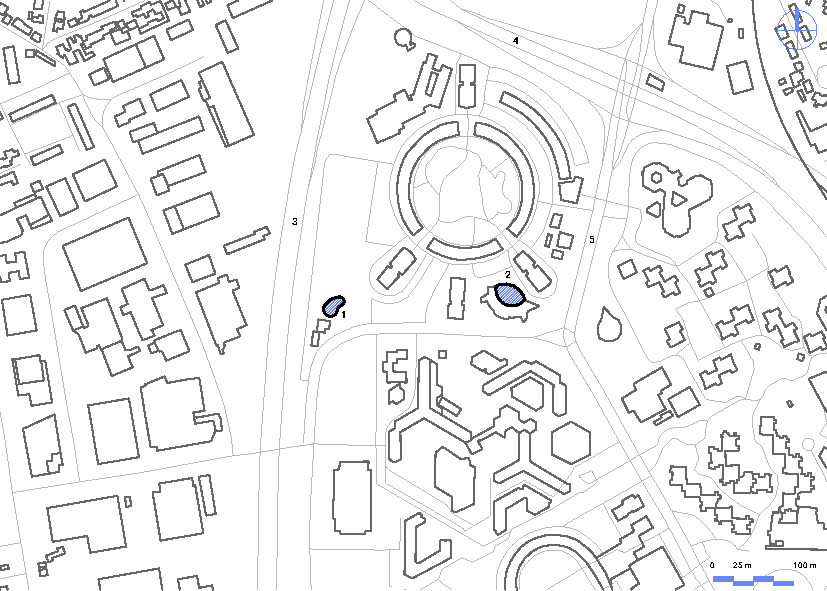
\includegraphics[width=1\textwidth]{situation_map}
		\caption{Situation map. The temporary gridshell (1) was built very close to the permanent cathedral (2). Remark that  the two buildings cover a quite similar projected area.}\label{fig:situation_map}    
		\vspace{1.5cm}
		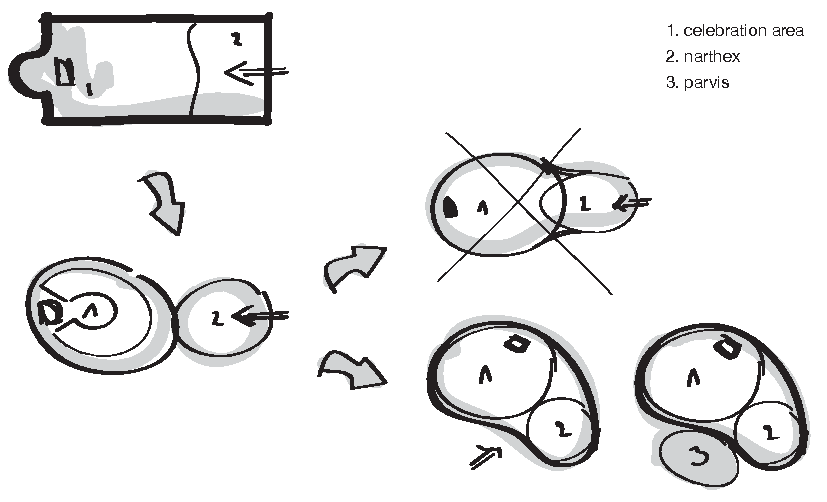
\includegraphics[width=0.7\textwidth]{form}
		\caption{Architectural sketch. Major and minor volumes are agglomerated into one volume. Here, the morphological register allowed by elastic gridshells appears to be relevant.}\label{fig:form}    
	\end{fullpage} 
\end{figure}

\section{Project overview}
%===================
\subsection{Context and challenges}
%----------------------------------------------
Creteil is a city of 90.000 inhabitants in the southeast suburb of Paris. Its urbanization began in the late 50’s, impelled by the French architect Charles-Gustave Stoskopf. In 1976 he designed Notre Dame of Créteil, a modest catholic church made of concrete, which became a cathedral 10 years later (see item 2 in \cref{fig:situation_map}). Recently, the diocese of Créteil has undertaken a major architectural redevelopment project of its cathedral, including a timber shell covering the religious area and the creation of a new cultural area. Once transformed, the edifice shall be more visible, more hospitable and livelier for citizens. Inevitably, such a molt takes time and a temporary place of worship was required to ensure liturgical services during the two-years work. In November 2011, T/E/S/S, the structural design office in charge of the cathedral renovation project, made an ambitious proposal to the diocese~: based on a previous successful experience – the construction of a composite gridshell for the festival Solidays \cite{Baverel2012} – T/E/S/S suggested that rather installing a basic tent, the parishioners should construct themselves a temporary cathedral.\footnote{See the video of the construction of Solidays' gridshell here : \url{https://youtu.be/24LLfcVIZWw}.}\textsuperscript{,}\footnote{See the video of the construction of Creteil's gridshell here : \url{https://youtu.be/jLq-UfOdnQQ}.}

\subsection{Architectural considerations on the form}
%------------------------------------------------------------------
The origin of this building form was driven by two objectives, that is, to provide a variety of appropriate internal spaces within which the community could assemble, and to provide an externally welcoming and visually interesting form. According to the architect Tom Gray, today, the internal organization of a roman catholic church is in large part driven by the post Vatican II vision of a religious celebration being a collective gathering of the community around the Eucharist, center of spiritual life. A circular seating arrangement is often considered the most convivial form to create a sense of belonging while minimizing a sense of hierarchy. However the community is not only using the building for religious celebration but also for encounters on a more informal manner, for example spontaneous gatherings after religious ceremonies. In the early Roman church, such gathering of the community was facilitated by the presence of an anti-space to the main space called a \emph{narthex}, through which one passed on entering the church. It was therefore felt appropriate that the formal freedom which the gridshell system offered would be used to explore forms composed of an agglomeration of major and a minor volumes which contain the two functions~: formal and informal gatherings (see item 1 and 2 in \cref{fig:form}).

Formal explorations were undertaken using modeling clay. The final form is based loosely on two adjacent semi spherical volumes of different size, which are merged into one complex form. Externally the fear of the design team was that the totally convex blob form could look intimidating. It was therefore decided that the two spherical virtual forms, which would be joined to make the final form, would be arranged not in a symmetrical axial manner, but in an asymmetrical curved composition. The resulting form seen in plan is convex on one side and concave on the other. The concave form in plan allows for double curvature to be introduced into what would be otherwise a simpler blob and gives sensuality and visual interest to the building.

\begin{figure}[p]
	\captionsetup[subfloat]{captionskip=10pt}
     	\centering
	\begin{fullpage}	
		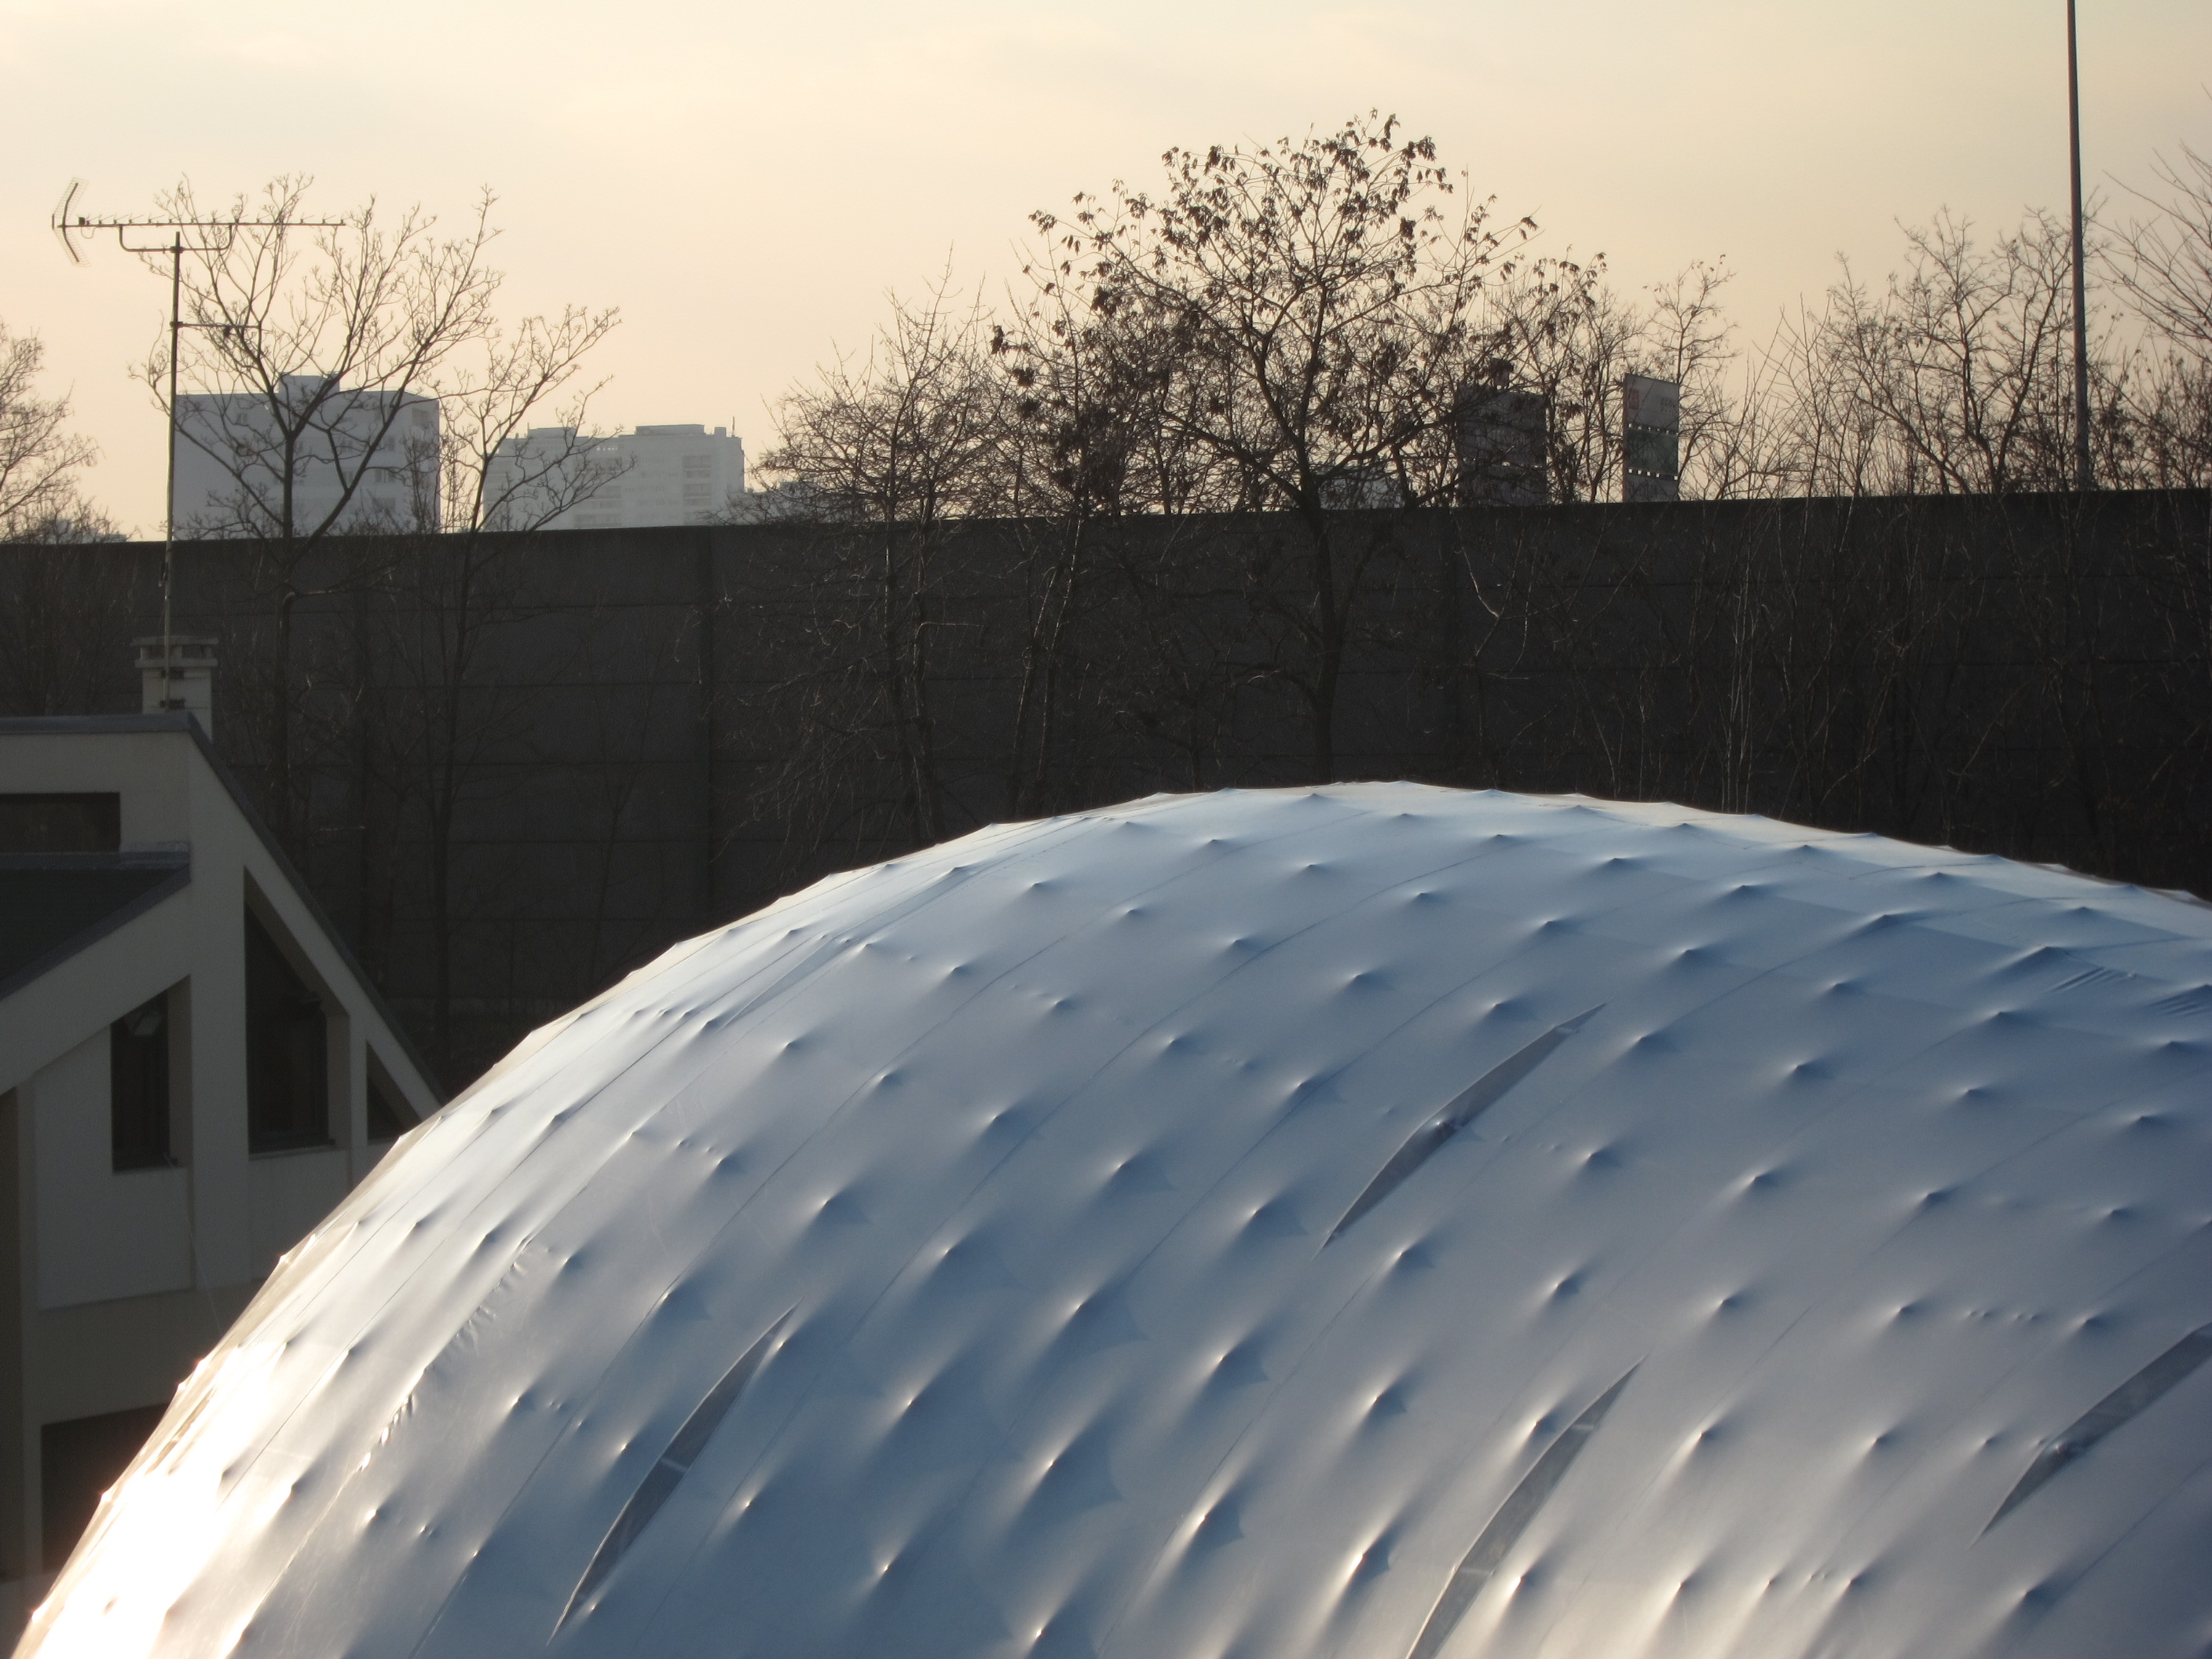
\includegraphics[width=0.80\textwidth]{gs_ext.jpg}
		\caption{Exterior view. The connections mark the fabric suggesting the interior grid structure. This texture enriches the perception of the building viewed from the outside and creates effects with the light reflections -- \textcopyright~L. du Peloux for T/E/S/S.}
		\label{fig:gs_ext}
		\vspace{1cm}
		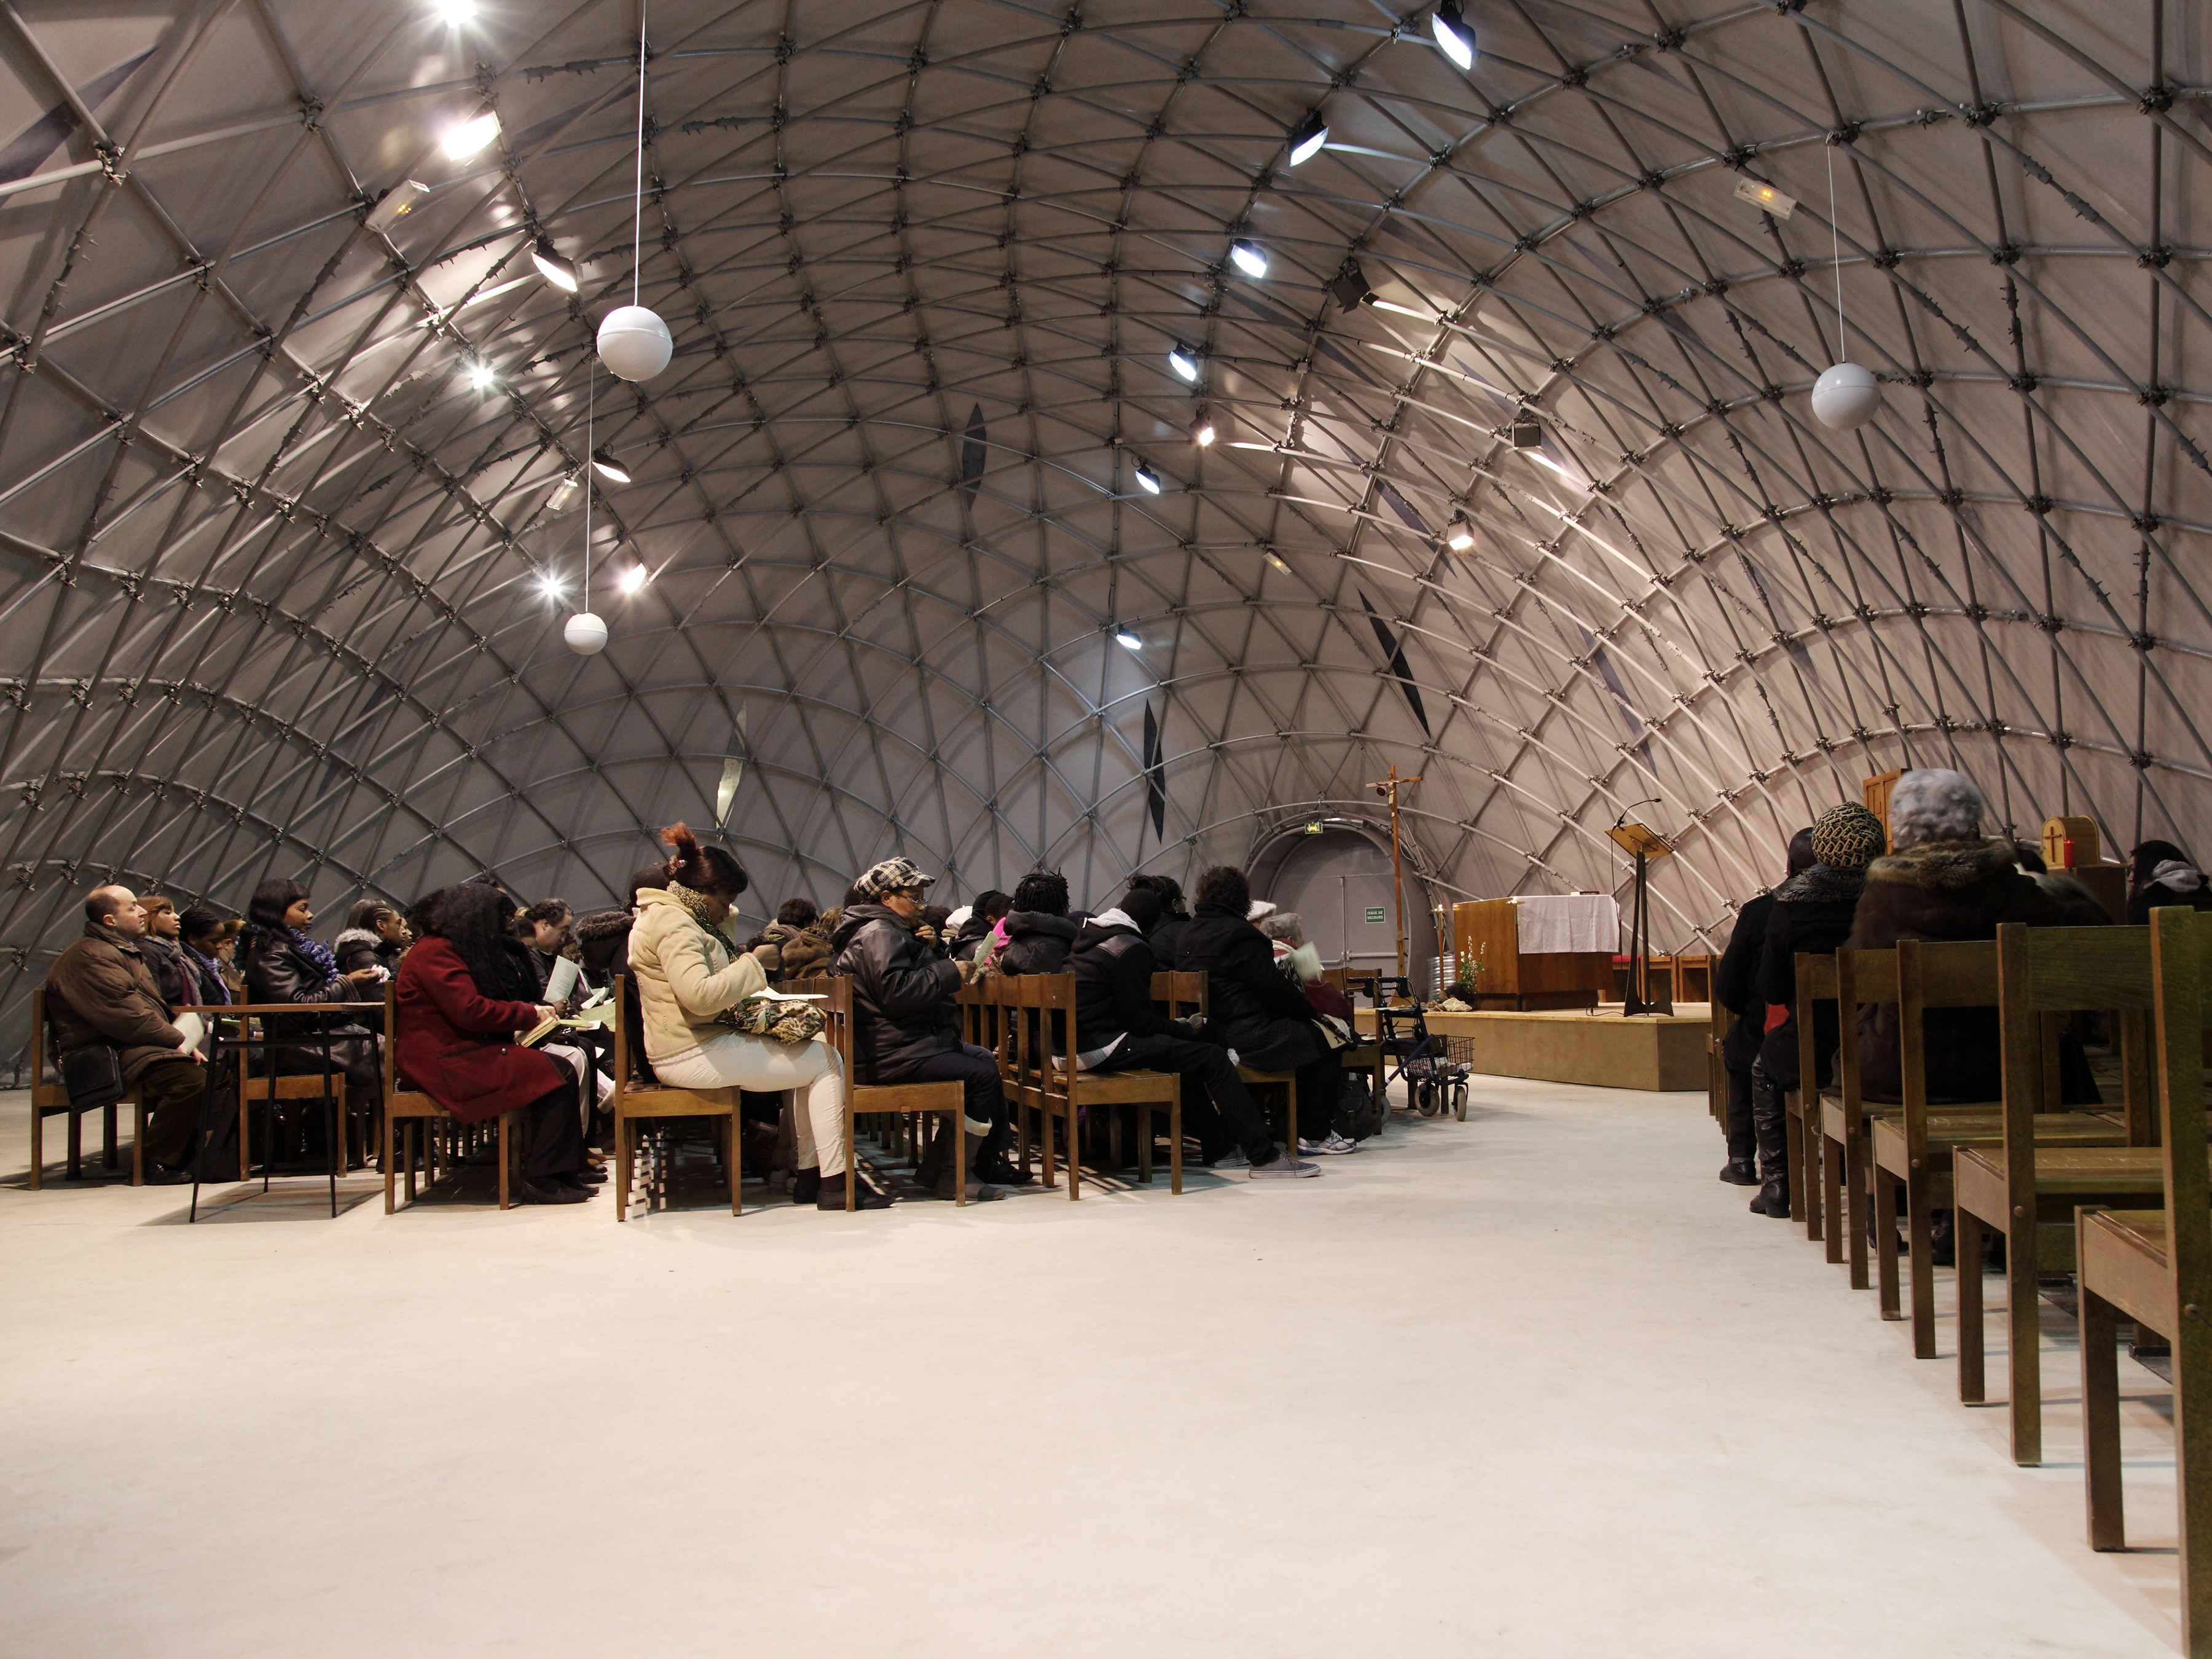
\includegraphics[width=0.80\textwidth]{gs_int.jpg}\label{fig:gs_int}
		\caption{Interior view. The grid pattern highlights the lightness of the structure and gives its tempo to the internal space. Lines converge to the altar, the heart of the liturgical area where the mass is offered on -- \textcopyright~C. Moissinac for T/E/S/S.}
		\vspace{20pt}
	\end{fullpage}
\end{figure}

\subsection{Placing of the building on the site}
The temporary cathedral is located on a land owned by the municipality, which is used for sporting and other communal gatherings. The curve in the building defines an external area where the church community could meet in the open air and this is where the entrance to the church is situated. The building was positioned on the site so that the entrance addresses a grass planted area forming a garden forecourt or “parvis” (see item 3 in \cref{fig:form}). A service building housing plant, toilets and vestry are housed in a port cabin positioned to the rear of the building (see \cref{fig:plan_view}).

\subsection{Entrance}
It is formally quite difficult to integrate doors, which must be verticals, into a complex geometry. Either the gridshell could be deformed to accommodate the geometrical requirements of doors, or the doors could be integrated into an independent form. The latter approach was chosen. In looking for forms to house the doors, reference was made to the conical monumental doorways with rings of concentric decoration, which welcome the faithful to romanesque and gothic churches in France. The conical forms were found to be coherent to the overall geometry of the building. The entrance doors were therefore inserted into a conical hooded form made of rolled steel plates and stiffened by concentric steel tubes, which not only make reference to historic precedence but also refer to the gridshell to be discovered inside (see \cref{fig:door_int}). The cone of the entrance doors was positioned in the concave side of the building giving access directly to the narthex part of the internal volume. To the rear of the church is situated a service door. The steel hood, which houses this door, is curved tightly around the door and takes up an ovoid form.

\subsection{Daylight}
The gridshell is covered in a PVC membrane, which is opaque. How to introduce daylight into the interior was a major subject of reflection. The simplest way found was to use transparent membrane placed occasionally on the membrane. A small amount of light was required in the interior to create a contemplative atmosphere. The lights would in consequence glow and would be seen as luminous insertions in the vault, like stars in the celestial vault or the apse of some Romanesque churches. The stars were patterned on the joints of the PVC membrane. The almond shape came from simplification of the cutting into the panels either side of the joints and to avoid stress concentrations around cuts in the membrane. This shape, known as Mandela, is frequently used in Marian religious imagery. The distribution of the transparent insertions is quite uniform but gets denser above the pinnacle.

\subsection{Technical description}
% ------------------------------------------

The gridshell structure is made of long glass fibre tubes (\O 42~mm) fastened together with scaffold swivel couplers (see, \cref{fig:swivel}). The structural members of the grid, all of different lengths, are built  from one, two or three composite tubes connected with steel sleeves (see \cref{fig:sleeve}). The length of the tubes is limited to 12~m to enable transportation through standard trucks. The tubes are organized in three layers. During assembly, the first two layers are first placed perpendicular to one another on the ground. They form the \emph{quadrangular primary grid}. The distance between the tubes of these two layers is constant, resulting in a regular grid. This primary grid is elastically deformed to obtain the final shape. The third layer of tubes acts as bracing. It gives the structure a shell-like behavior. The tubes are fixed to the primary grid once the shape has been obtained

The structure is anchored to a concrete strip footing with a special anchorage system, which ensures transfer of loads from the composite structure to the ground (see \cref{fig:anchorage}). A similar system enables fixation of the structure to the doors (see \cref{fig:door_int}).

A PVC coated fabric (see \cref{fig:gs_ext}), tailor-made for the purpose, covers the structure. The transparent portion of the structure allows daylight inside the gridshell. The fabric is stretched on the peripheral edge of a dedicated beam with a double-lacing system (halyard and strap, see \cref{fig:edge}). At the ground level, the lacing edge of the beam is made of a bent, composite rod nailed to the concrete slab. At the grid–door junction, a steel arch is welded to the doorframe (see \cref{fig:door_ext}).

The PVC fabric is waterproof and, since it is a continuous membrane, has no joints except at the perimeter. At the perimeter, a continuous strip of membrane is prefixed to the internal surface of the membrane and fixed to the ground slab. At the doors, a flexible strip of the membrane is riveted to the doorframe.


\begin{figure}[p]
	\captionsetup[subfloat]{captionskip=10pt}
     	\centering
	\begin{fullpage}	
		%
		\subfloat[][Exterior.]{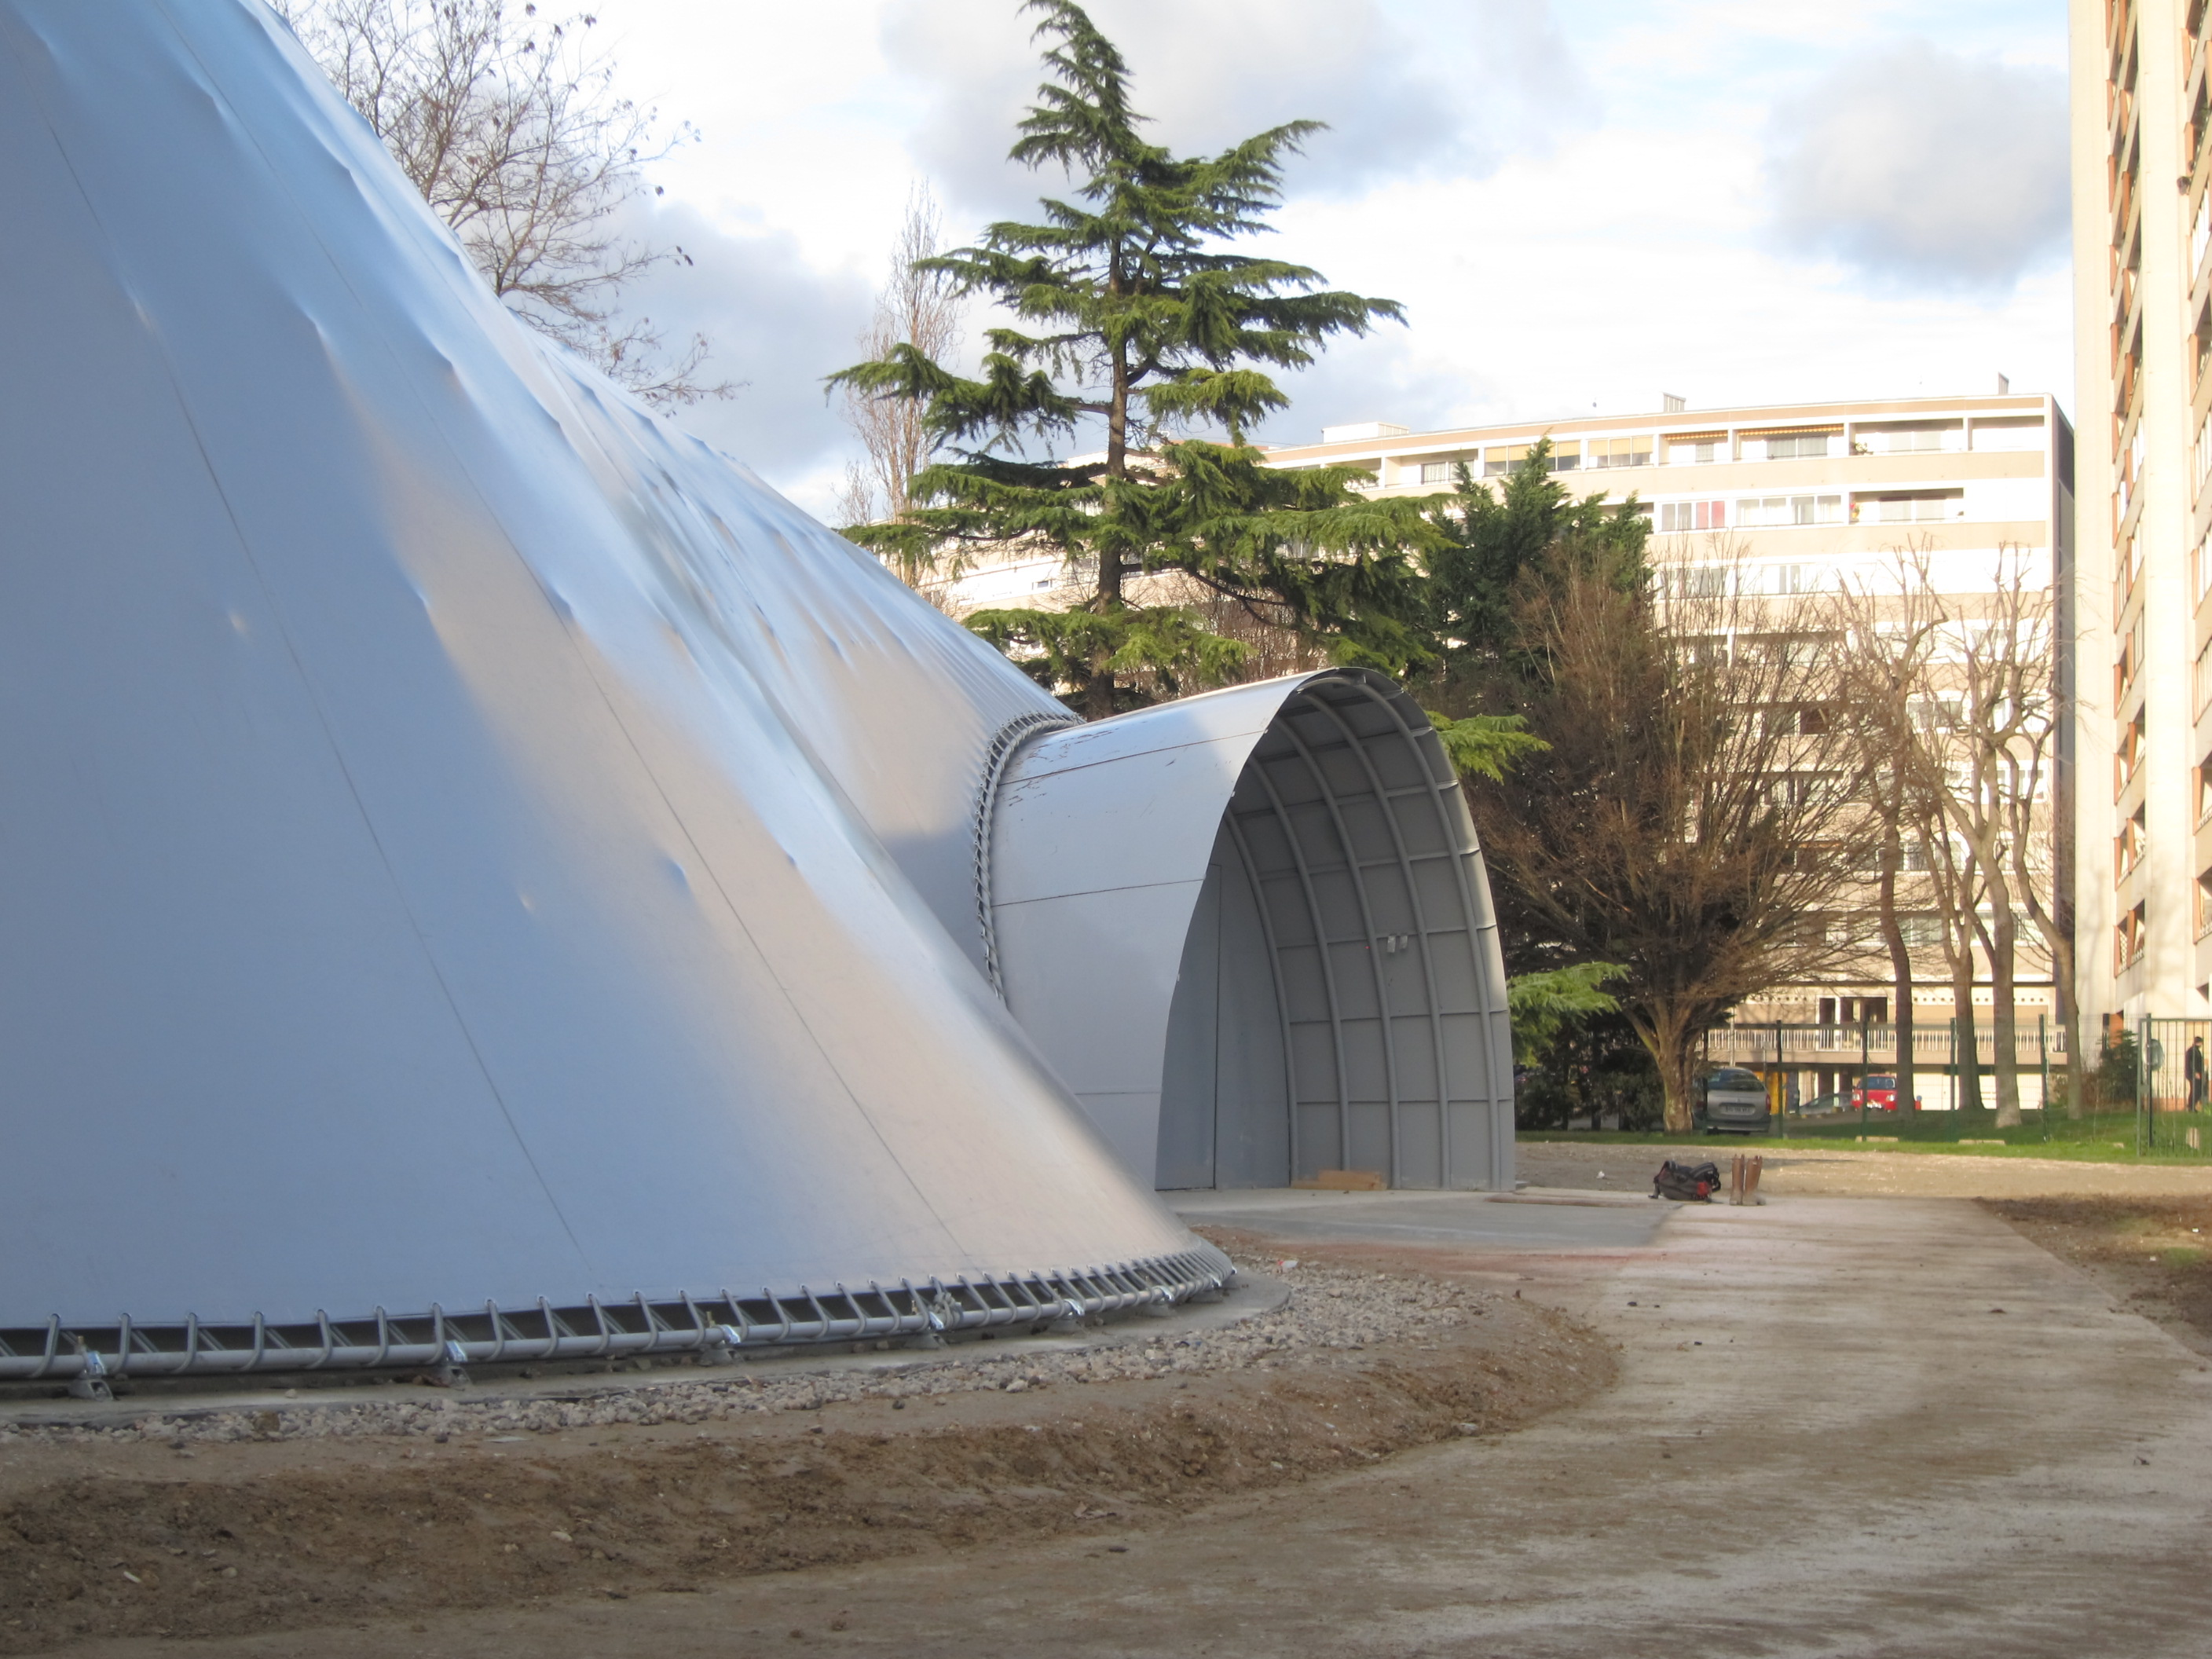
\includegraphics[width=0.48\textwidth]{door_ext.jpg}\label{fig:door_ext}}
		\hspace*{\fill}
		\subfloat[][Interior.]{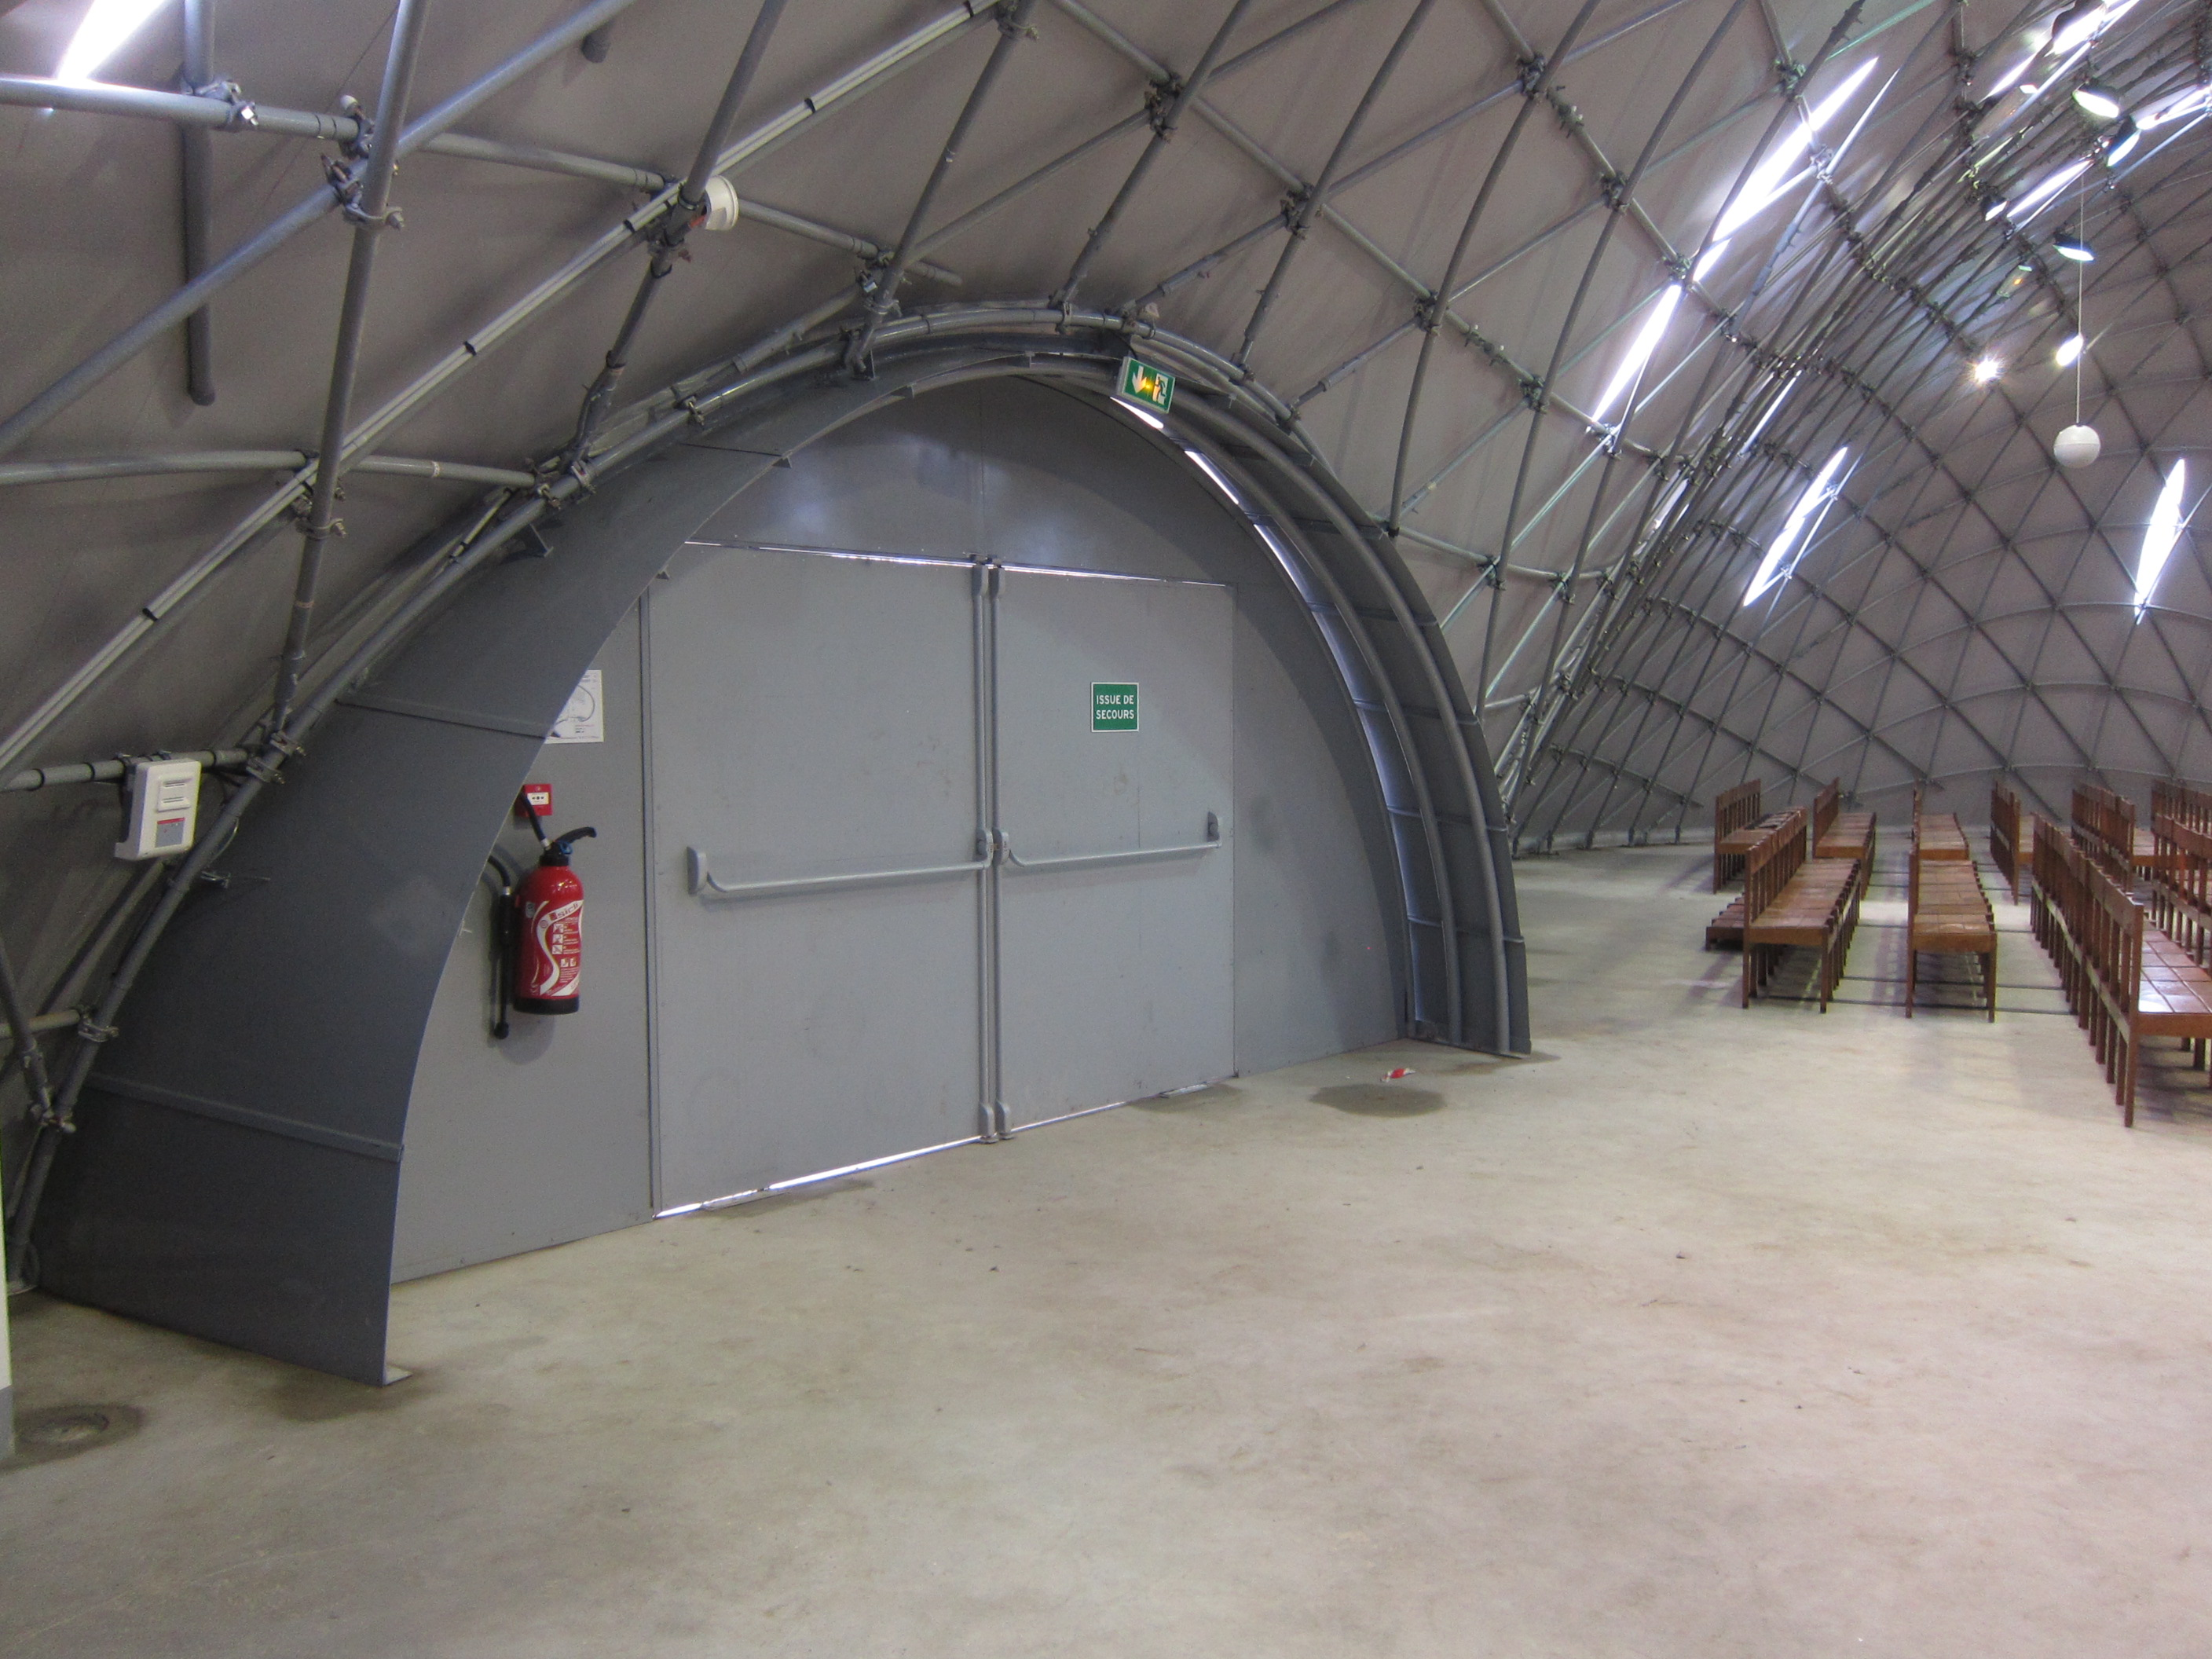
\includegraphics[width=0.48\textwidth]{door_int.jpg}\label{fig:door_int}}
		\vspace{10pt}
		\caption{Entrance. Two steel doors allow the entrance inside the building.}
		\label{fig:door}
		%    
     		\vspace{1cm}
		%
		\subfloat[][Swivel coupler.]{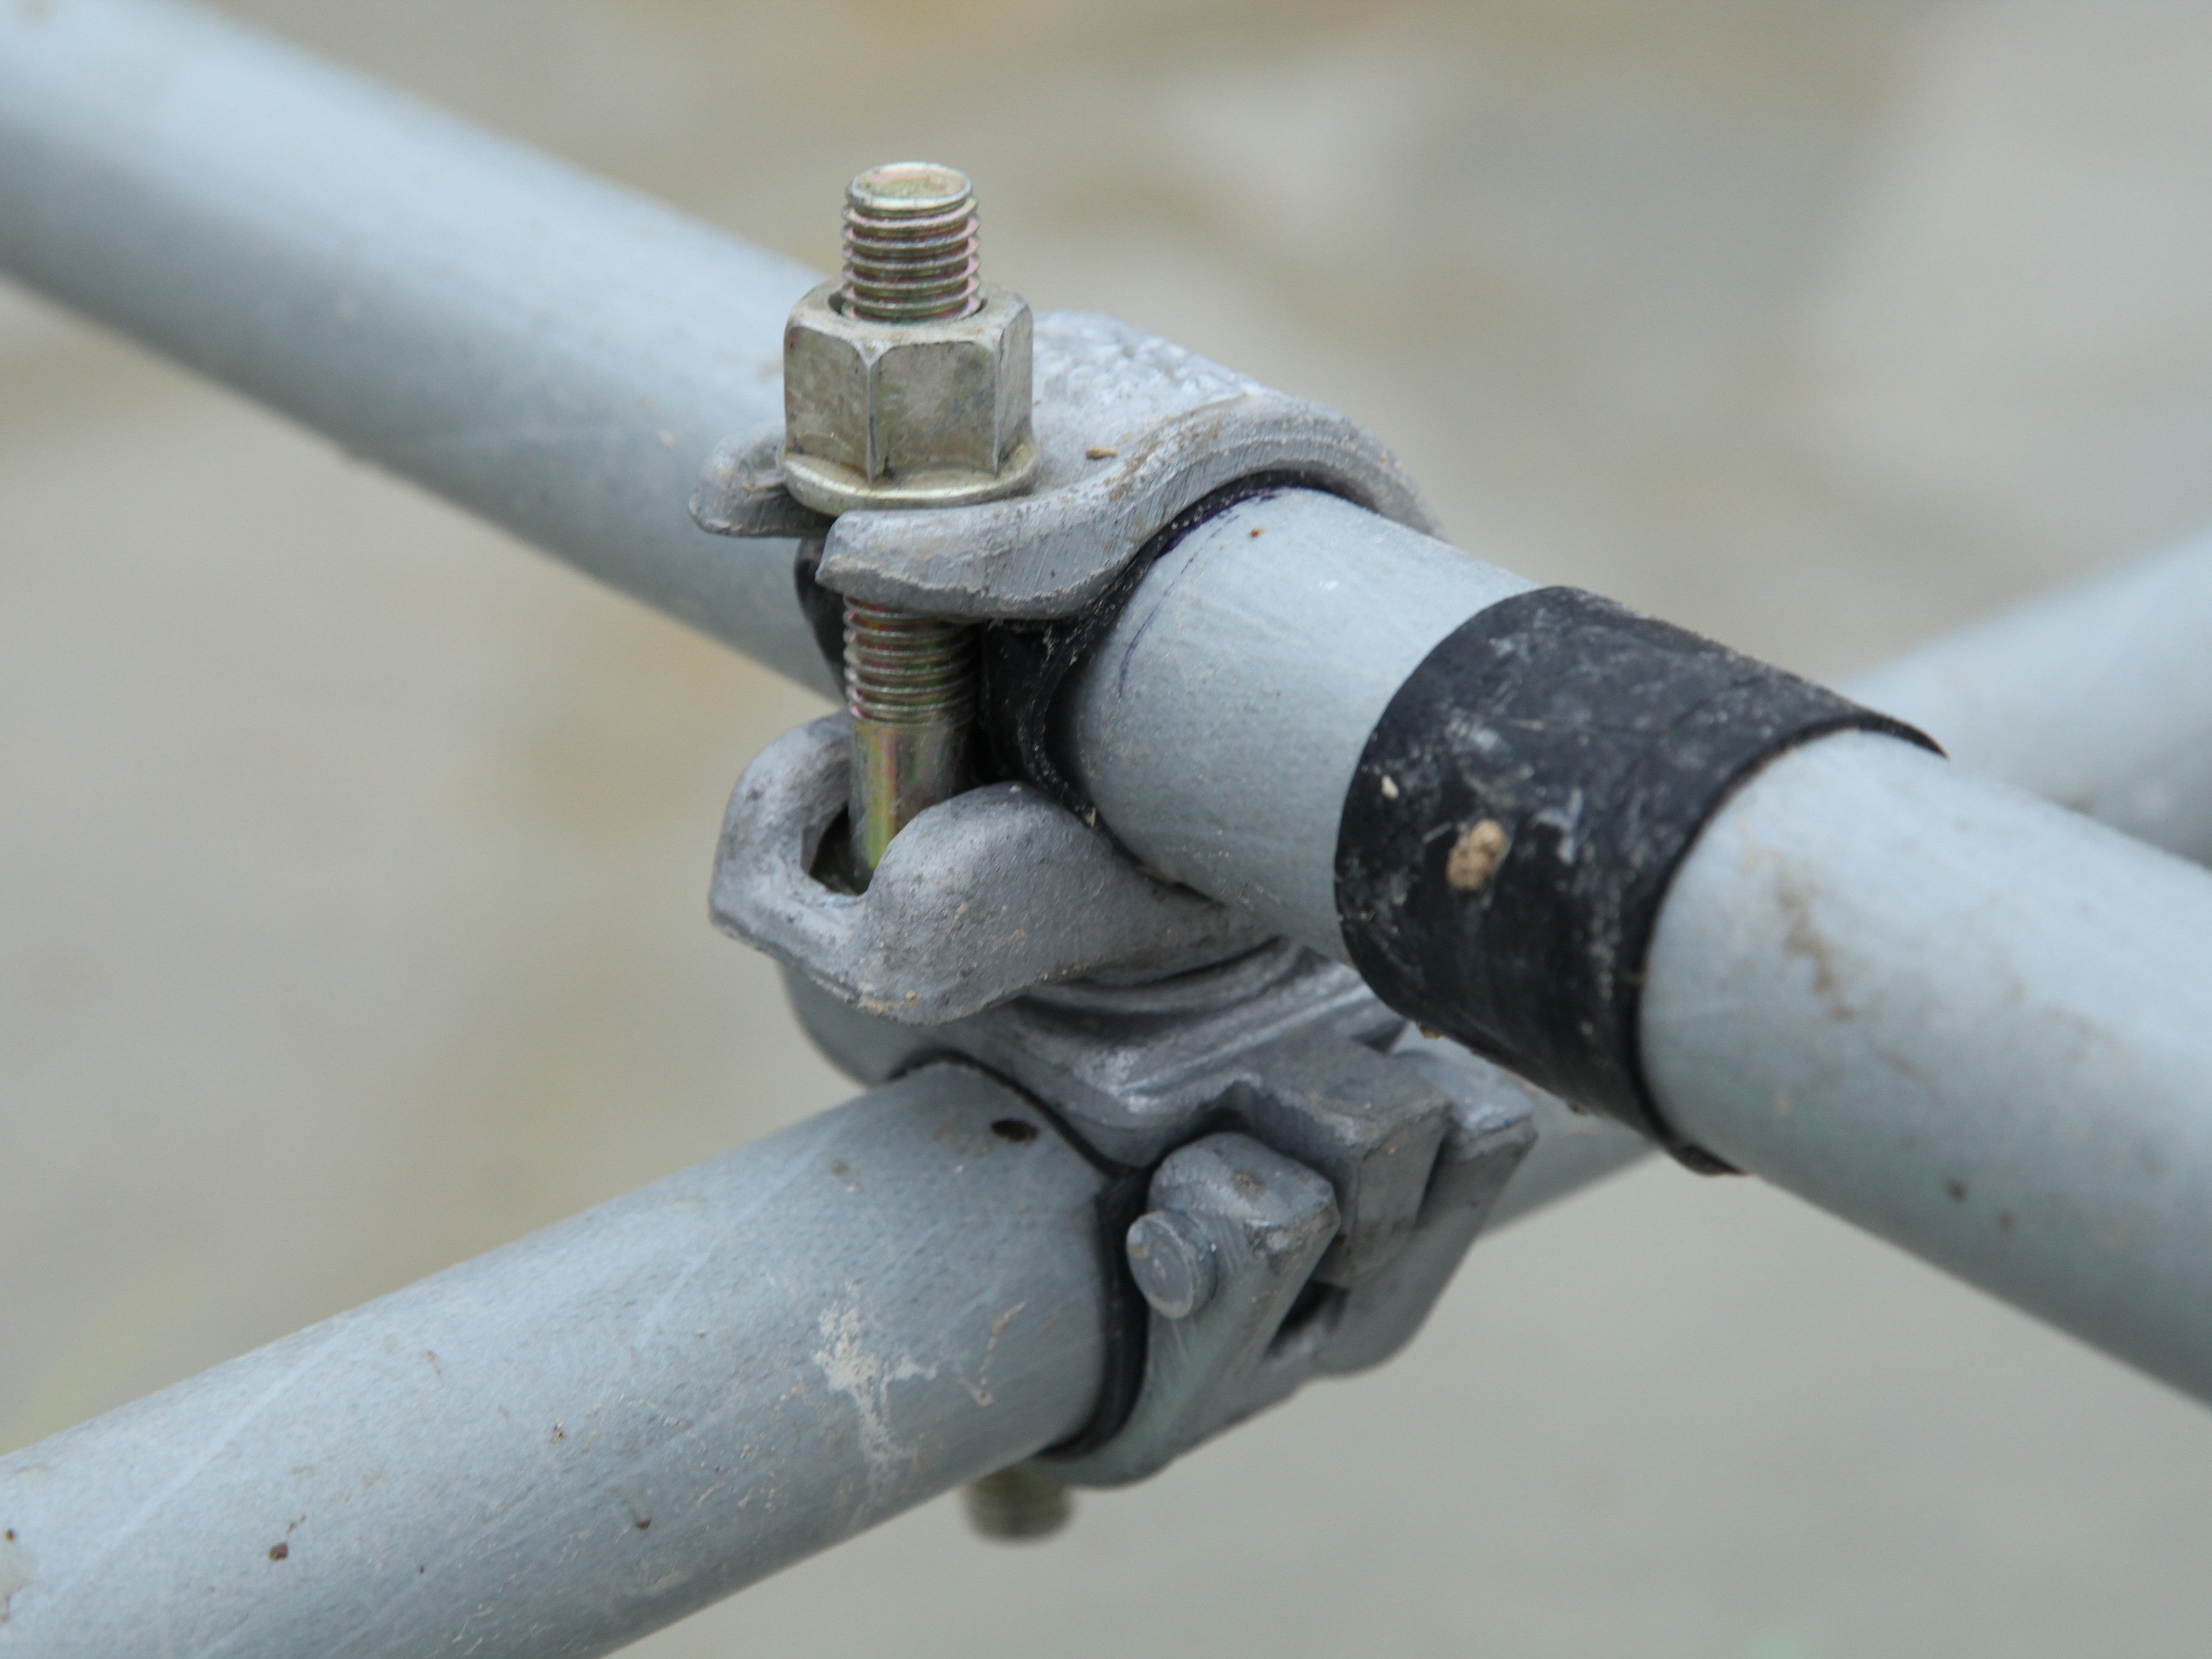
\includegraphics[width=0.48\textwidth]{swivel.jpg}\label{fig:swivel}}
		\hspace*{\fill}
		\subfloat[][Sleeve system.]{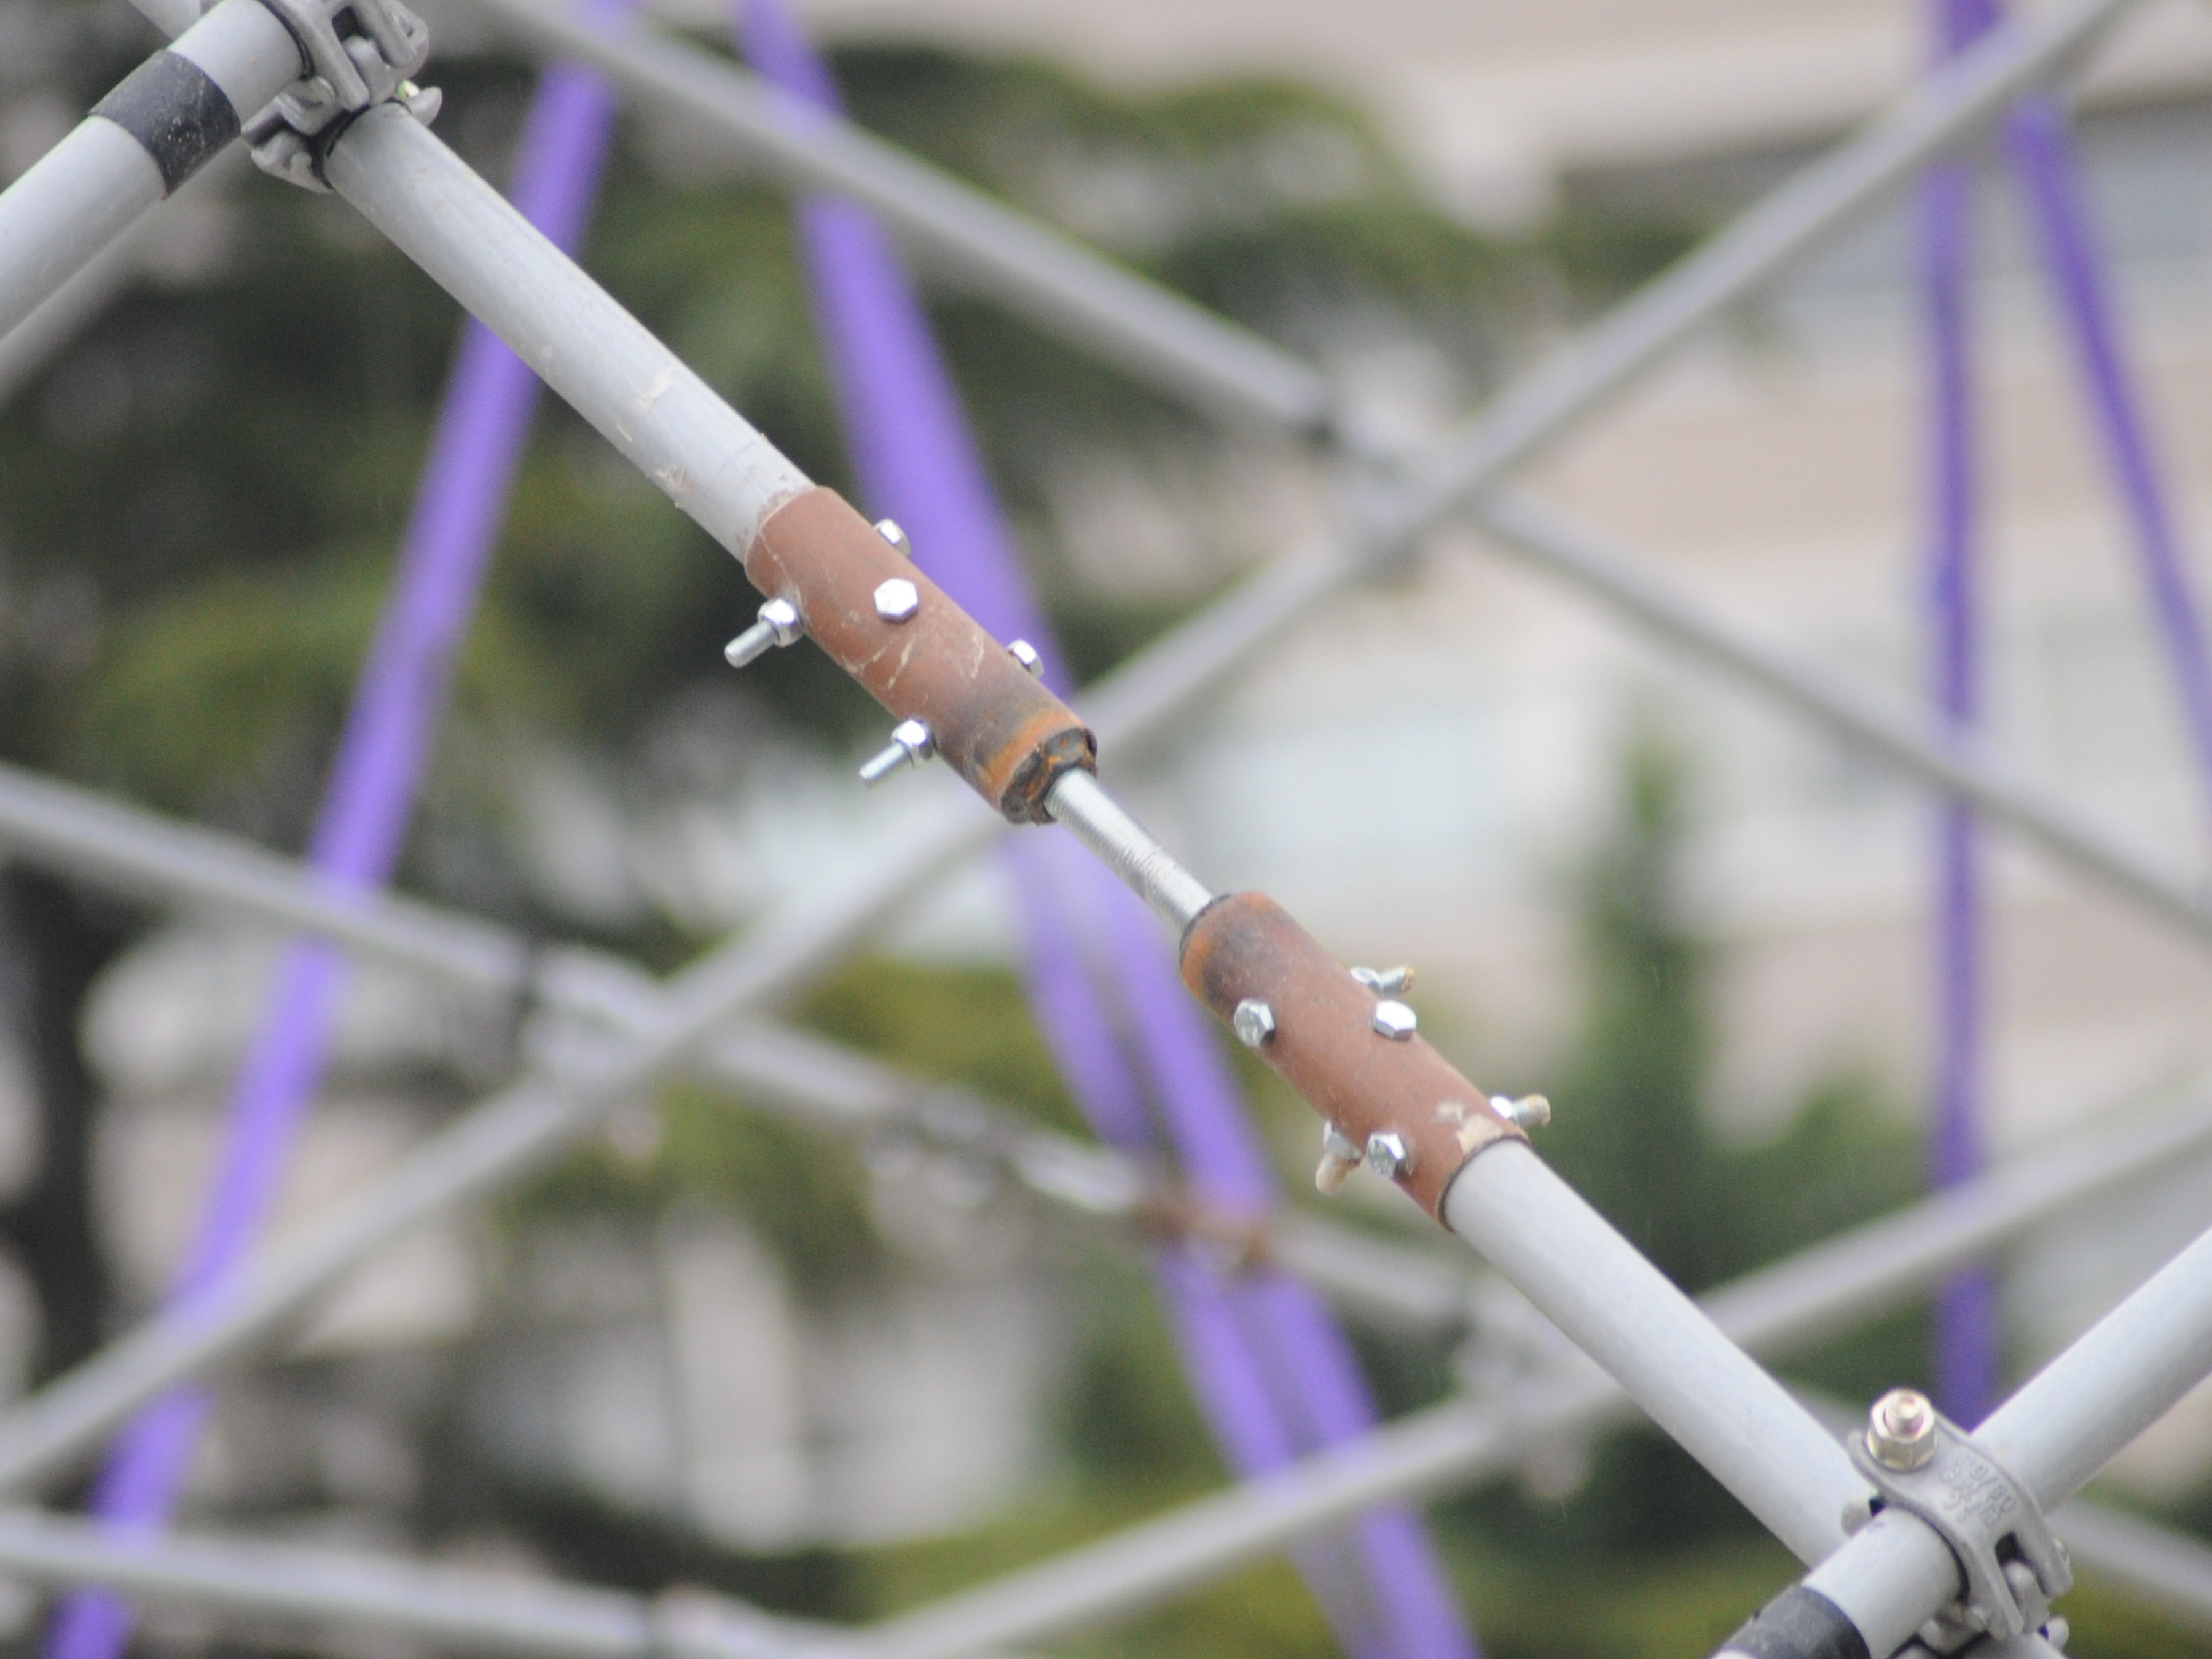
\includegraphics[width=0.48\textwidth]{sleeve.jpg}\label{fig:sleeve}} \\
		%
		\subfloat[][Ground anchorage.]{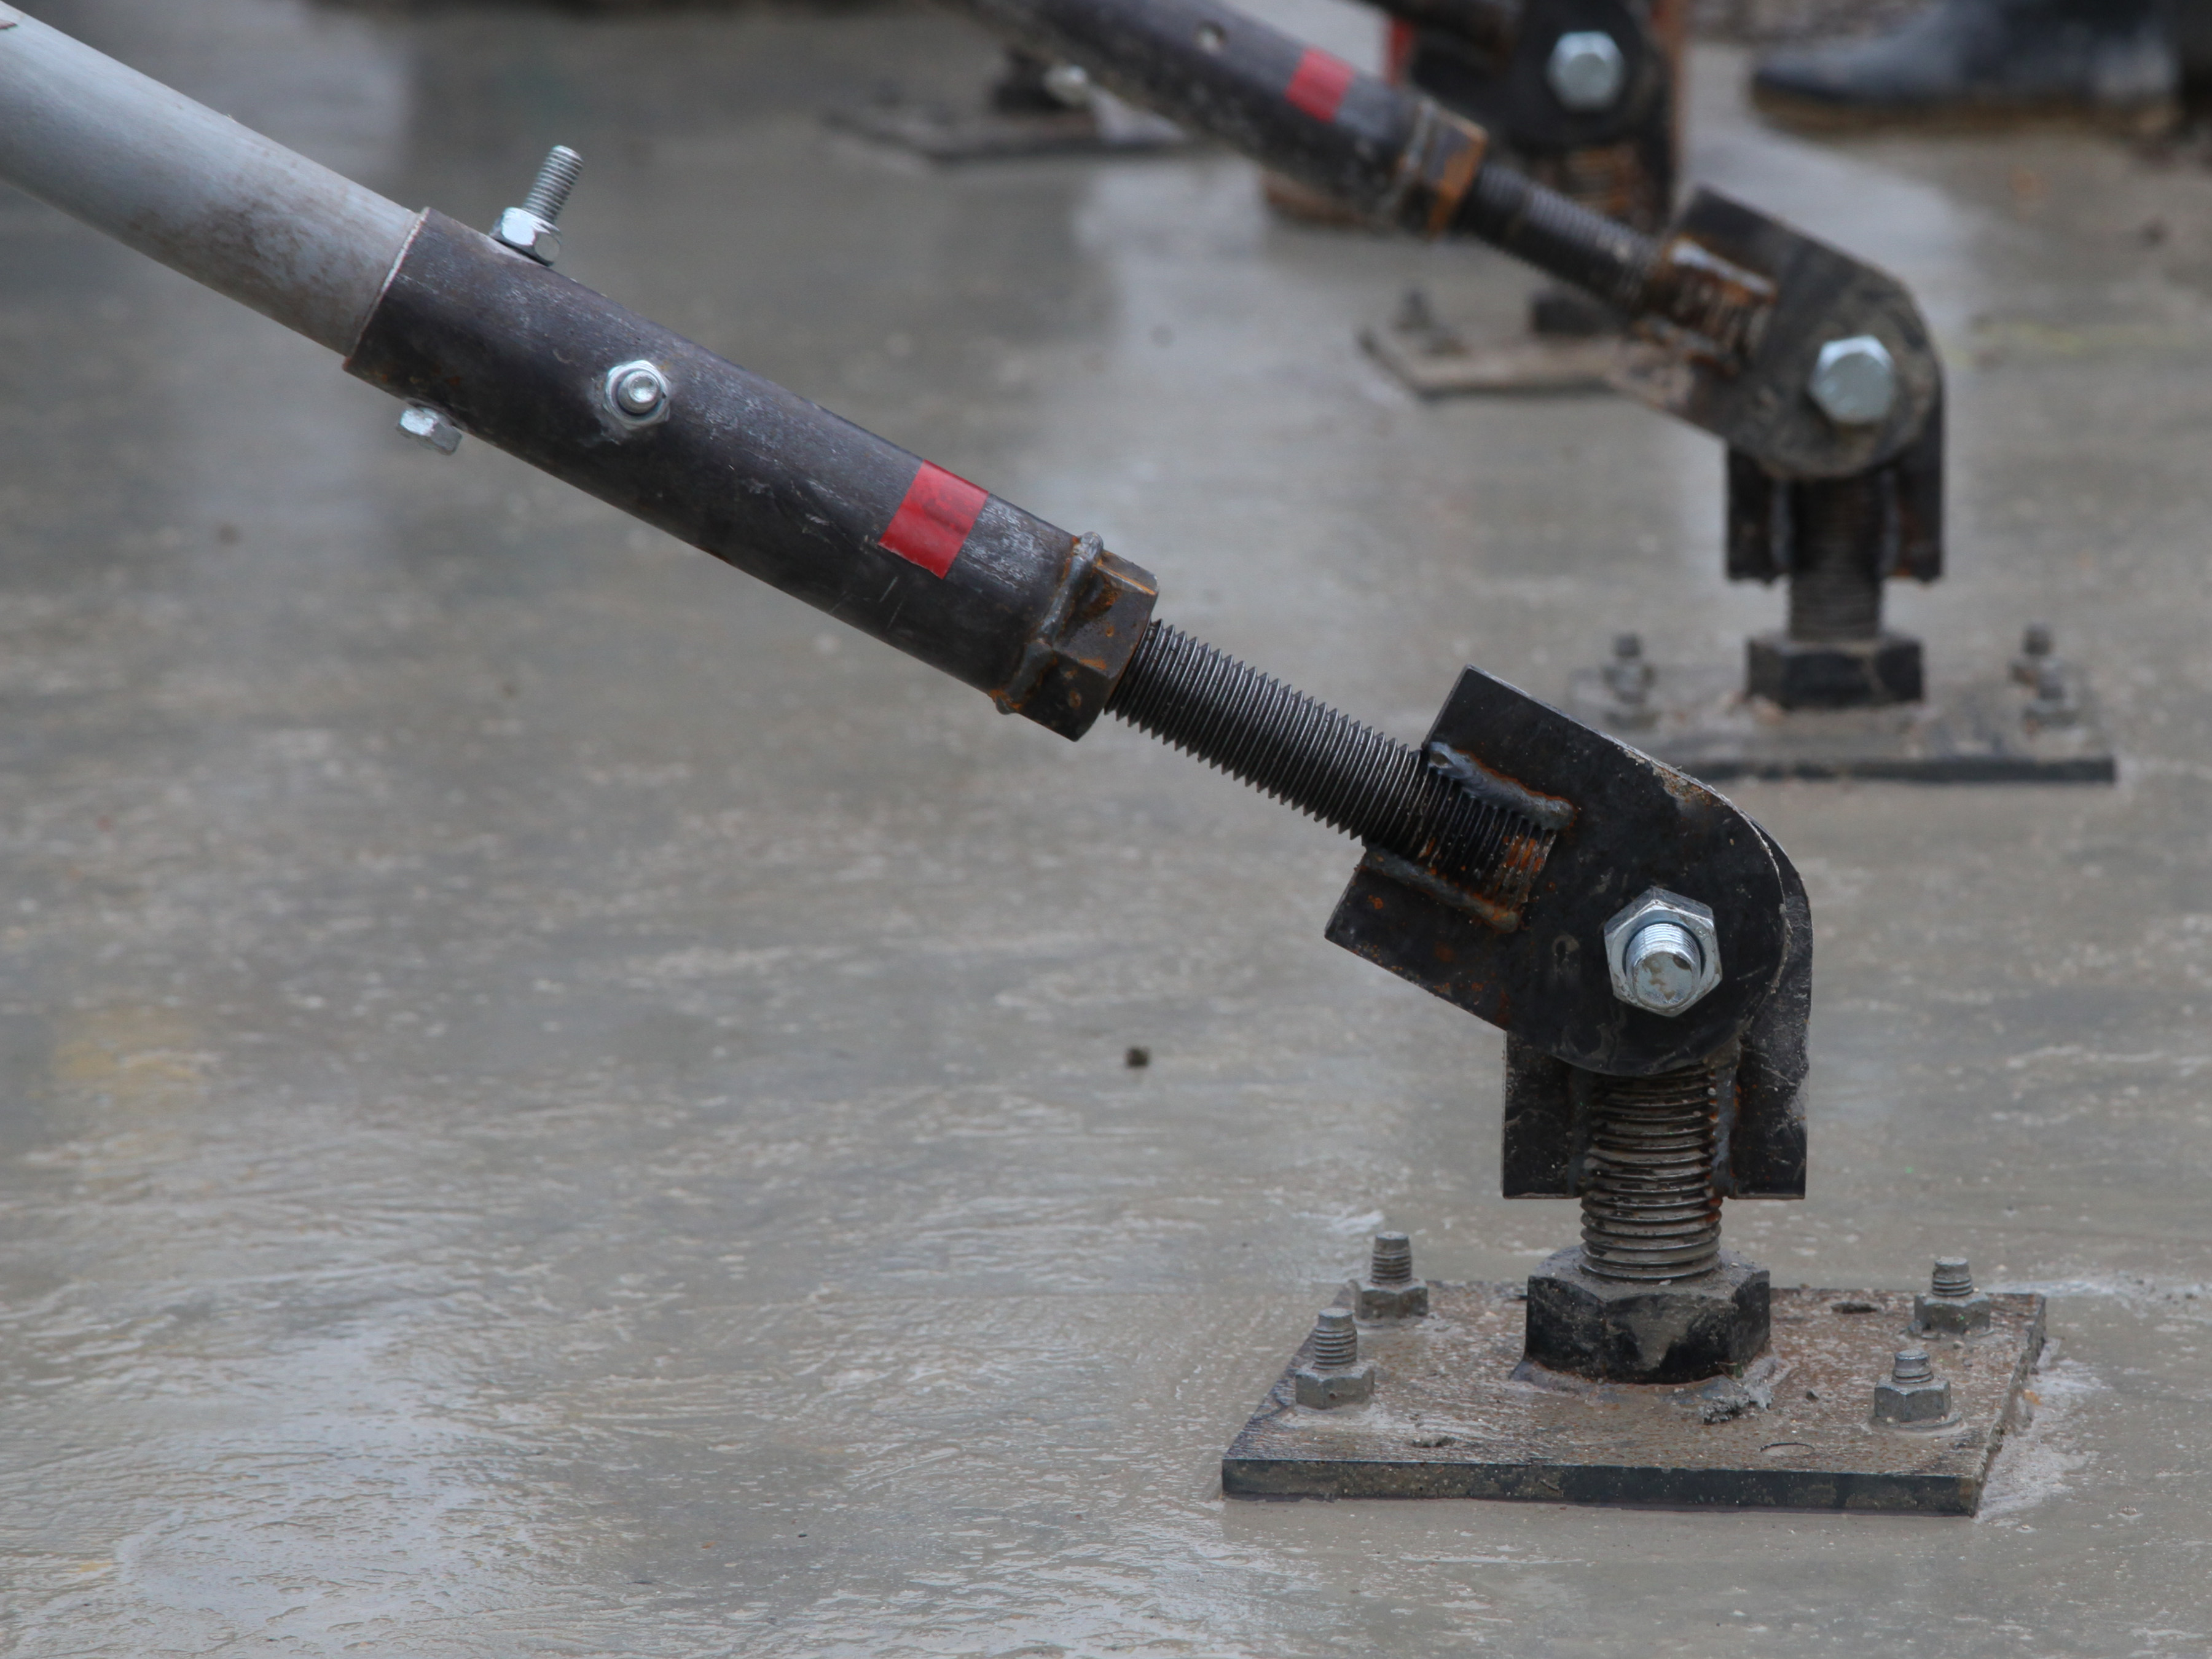
\includegraphics[width=0.48\textwidth]{anchorage.jpg}\label{fig:anchorage}}
		\hspace*{\fill}
		\subfloat[][Lacing rod.]{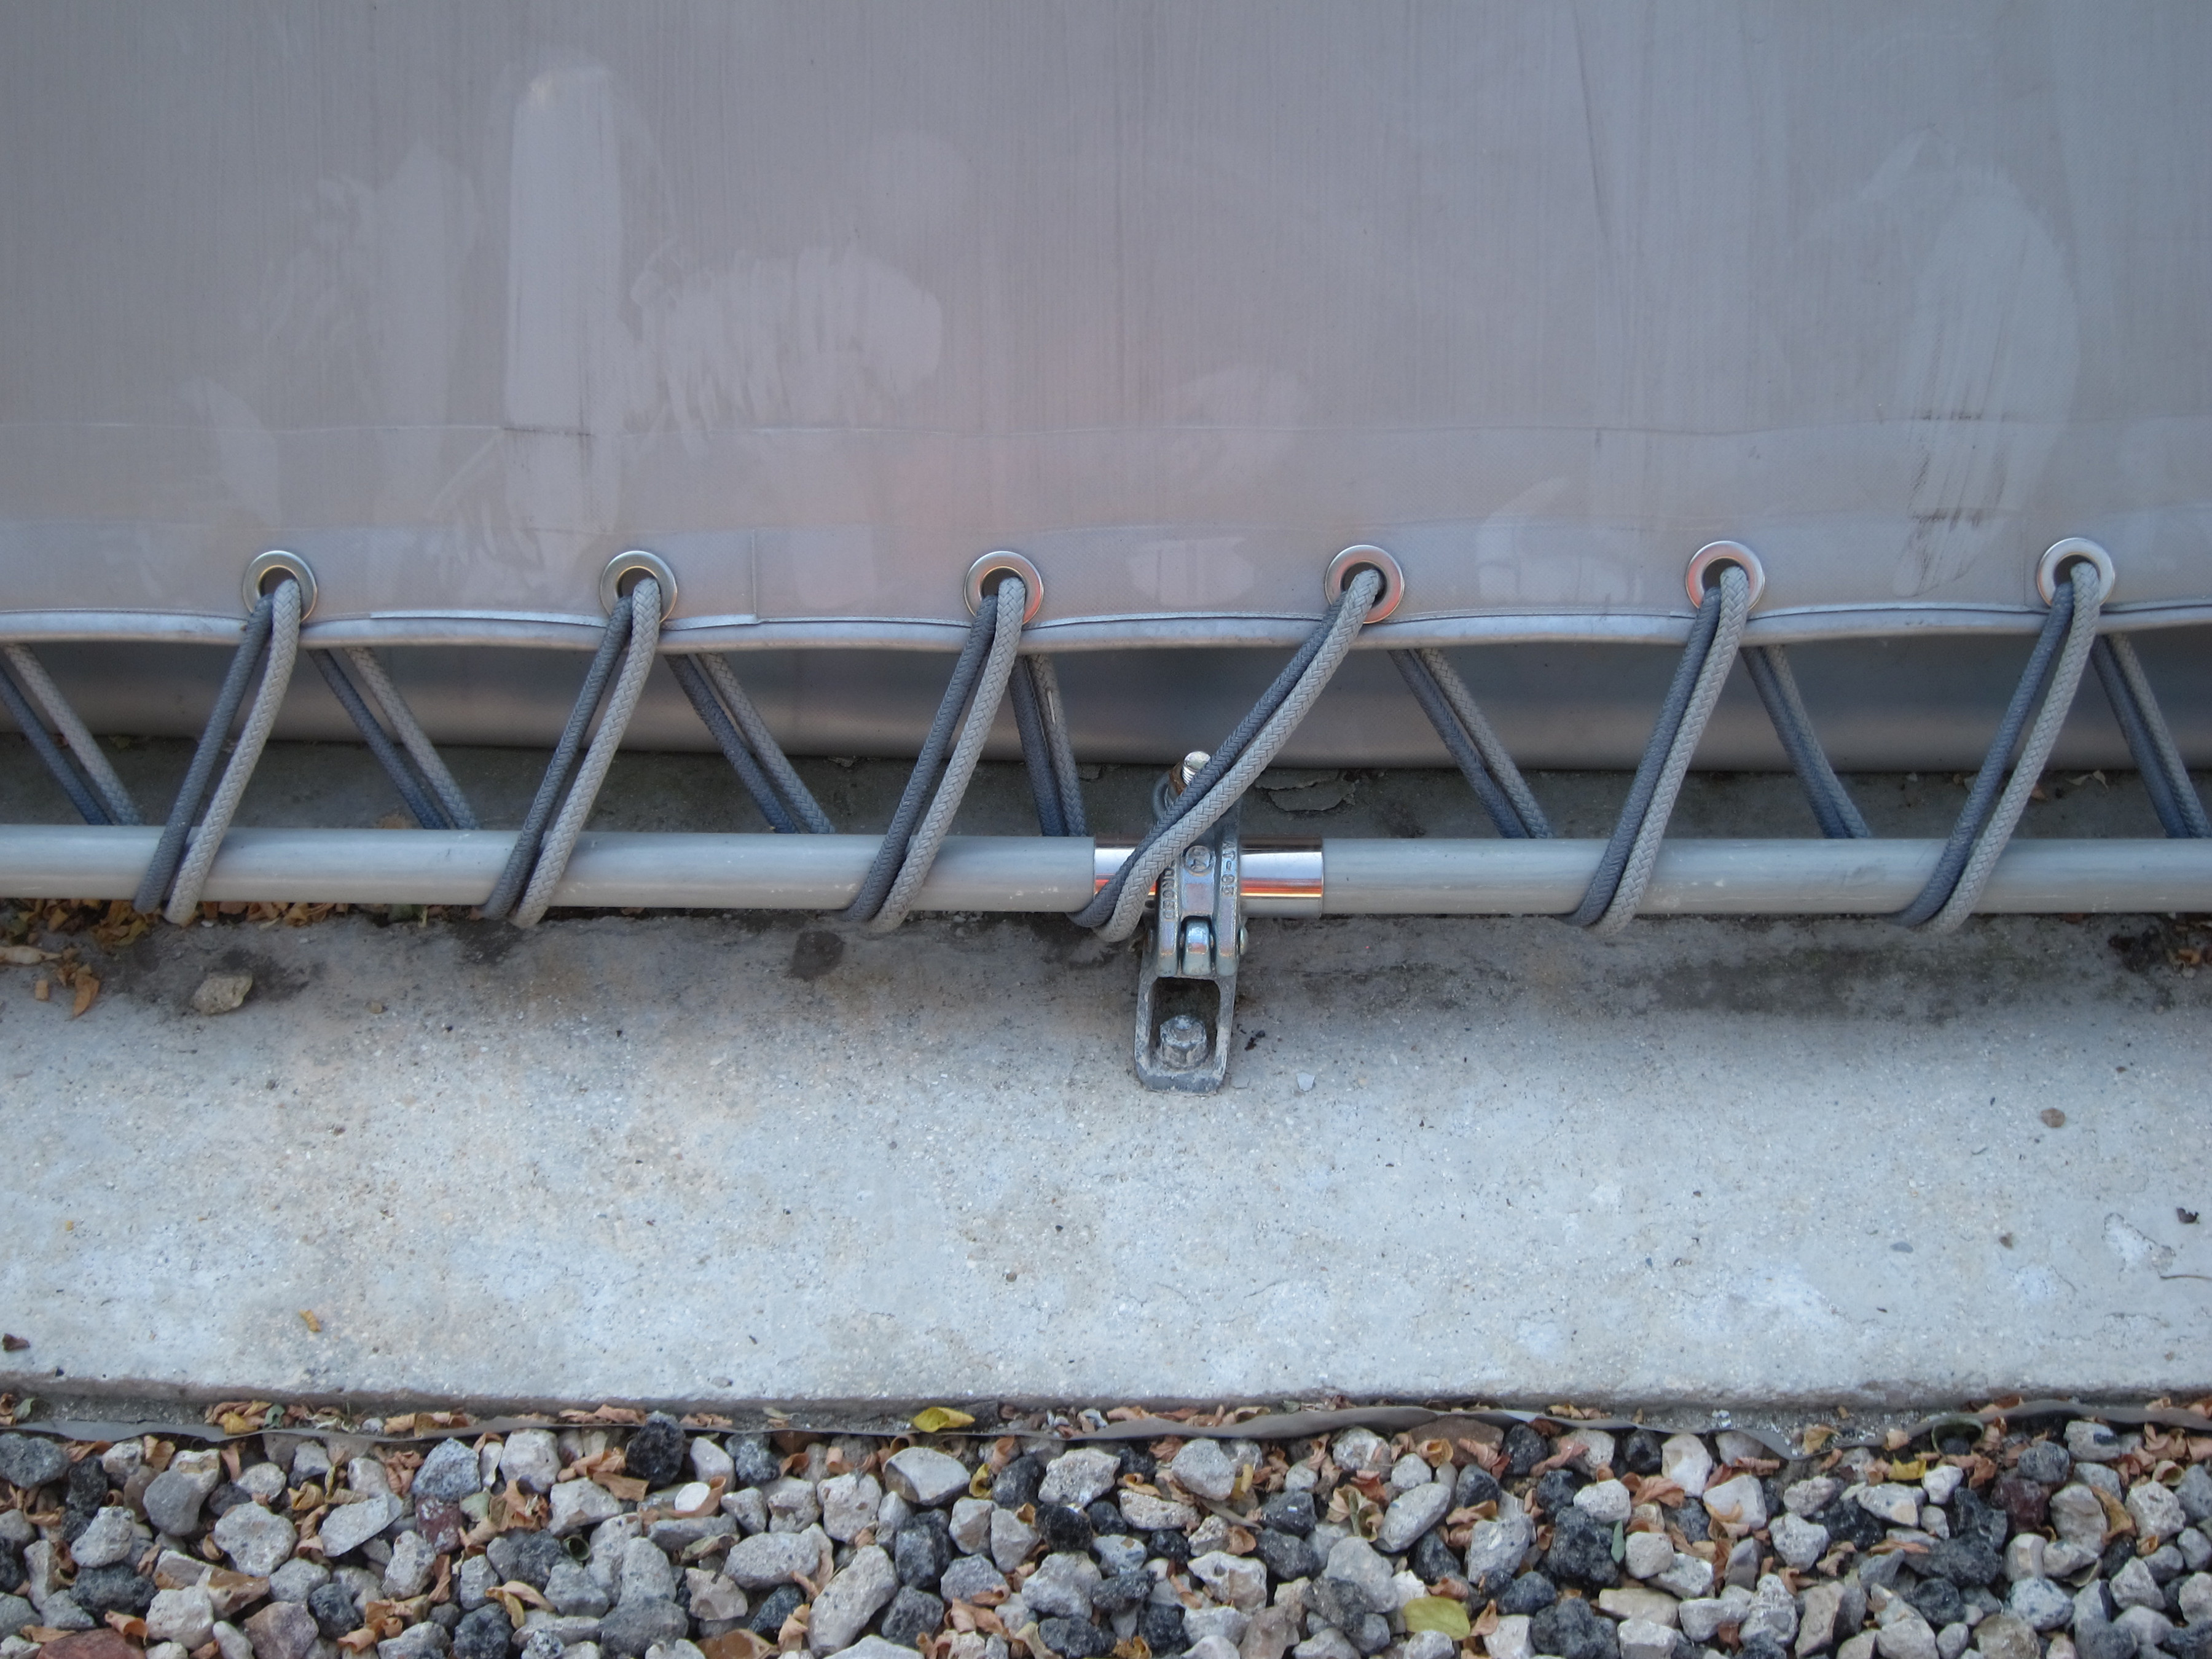
\includegraphics[width=0.48\textwidth]{edge.jpg}\label{fig:edge}} \\
		%
		\vspace{10pt}
		\caption{Standard elements that composed the structural system.}
		\label{fig:parts}    
	\end{fullpage}
\end{figure}

\begin{figure}[p]
	\captionsetup[subfloat]{captionskip=20pt}
     	\centering
	\begin{leftfullpage}	
		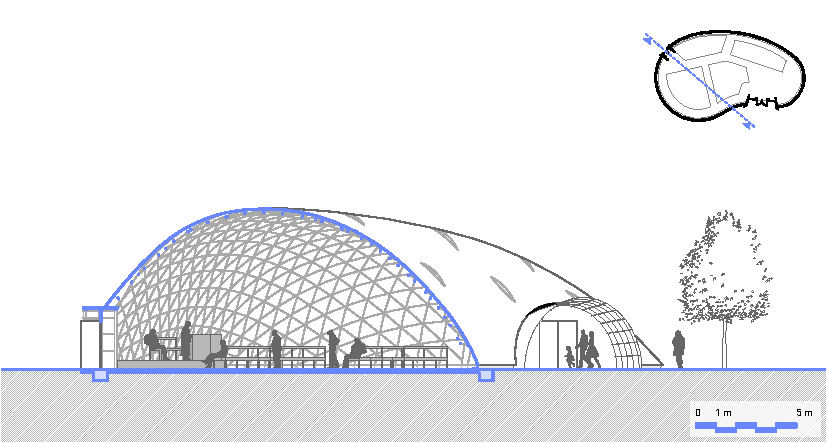
\includegraphics[width=\textwidth]{section_view}
		\caption{Transversal section of the building. Observe how the grid gets denser at the choir. Two doors give access to the building. The height at the pinnacle is about 7~m.}
		\label{fig:sec}
		%
		\vspace{1.5cm}
		%
		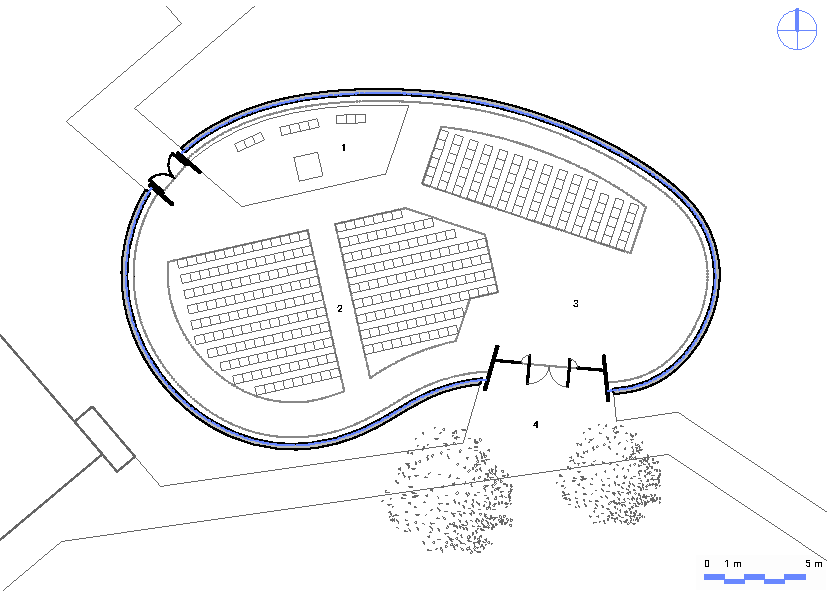
\includegraphics[width=\textwidth]{plan_view}
		\caption{Top view of the building. The interior space is composed of a choir (1), a place of assembly (2) and a narthex (3). The main entrance overlook the parvis (4). The shell spans about 29~m in the longitudinal direction and about 17~m in the transversal direction. The covered area is about 350~m\textsuperscript{2}. The space can accommodate 360 seating people or 500 standing people.}
		\label{fig:plan_view}	
	\end{leftfullpage}
\end{figure}
\begin{figure}[p]
\centering
\ra{1.1}
\begin{fullpage}
 	\begin{tabular}{@{}lllrr@{}}
	\toprule
 	Category	 	& Item 						& Unit 		& Quantity\\ 
	\midrule
	Public  		& seating  					& p					& 360 \\
      				& standing 					& p					& 500 \\
	\midrule
	\addlinespace[0.5cm]
	Dimensions   	&  length						& m 					& 29	\\
	   			&  width 						& m					& 17	\\   			
				&  height 						& m					& 7	\\
				& contour 	 					& ml					& 75\\
				& area						& m\textsuperscript{2}	& 350\\
				&  volume						& m\textsuperscript{3}	& 1600 \\
	\midrule
	\addlinespace[0.5cm]
	Gridshell   	&  tubes (x176)					& ml					& 1775 \\
	   			&  connections					& 					& 1130 \\   			
				&  sleeves						& 					& 125 \\
				& anchorages 					& 					& 127 \\
				& \quad \emph{ground (single)} 	& 					& 77 \\
				& \quad \emph{ground (double)} 	& 					& 16 \\
				& \quad \emph{door (single)} 		& 					& 18 \\
				& weight  						& kg/m\textsuperscript{2} 	& 5 \\
	\midrule
	\addlinespace[0.5cm]
	Fabric   		&  opaque						& m\textsuperscript{2}	 & 530 \\
	   			&  transparent					& m\textsuperscript{2}	& 12 \\ 
				&  lacing rod					& ml 				 	& 67 \\  			
				& weight						& kg/m\textsuperscript{2}	& 1 \\
	\bottomrule
 	\end{tabular}
\caption{Key numbers.}
\end{fullpage}
\end{figure}


\section{Construction process}
% ====================

The first two directions of tubes were assembled perpendicularly on the ground with the swivel couplers (see \cref{fig:swivel}) to form the \emph{primary} grid. The resulting grid covered about 600~m\textsuperscript{2} (see \cref{fig:cp_1}). At each intersection, the tubes were fastened together with a coupler, installed manually by the volunteers. They were asked not to tighten the bolts but just to engage the collars in order to prevent potential damages from the collar over the tube. Once the assembly of the primary grid was complet, the swivel couplers were tightened with a torque wrench to the optimal torque specified specified by the laboratory Navier. The whole stage took two full days. Note that because the anchorages sticked out from the slab, it was decided not to assemble the grid on the concrete slab to ensure that the grid would be able to slide freely on the ground and not get clung in the anchorages during the erection stage.

The next stage consisted in lifting the grid simultaneously with two mobile cranes (35t). Once lifted up, the grid took nearly its final form (see \cref{fig:cp_2}). The structure was slowly moved above the slab until tube endings faced at best their respective anchor points. Then, tube after tube, the workers pined the grid to the ground anchorages (see \cref{fig:cp_3}). This stage is tricky, especially at the beginning because only few tubes are connected to the ground. If the grid moves it can easily break these few tubes. The action of pinning a tube is done with a single bolt. The end of each composite tube is equipped with a rotating steel clevis. Similarly, each ground anchorage is composed of a steel plate fixed to the concrete slab and a rotating clevis. To pin a tube to an anchorage, their clevis are aligned one to each other and a pin is positioned in their central hole (see \cref{fig:anchorage}). When all the tubes were pinned to their anchorage, the grid was stable and secured and the cranes were removed (see \cref{fig:cp_4}). The stage lasted one full day.

Once the primary grid was deformed into the final shape, it was braced by a third direction of tubes called the \emph{triangulation}. The triangulation tubes split the quadrangular mesh of the primary grid into triangles (see \cref{fig:cp_5}). This work was tedious as it required working at height in aerial buckets. Tubes were hand-conveyed in the structure and attached to the tubes of the second layer with an additional swivel coupler. Each node of the structure would then be composed of two connections (see \cref{fig:swivel_dwg}).



\begin{figure}[p]
	\captionsetup[subfloat]{captionskip=10pt}
     	\centering
	\begin{fullpage}	
		\subfloat[][Flat grid.]{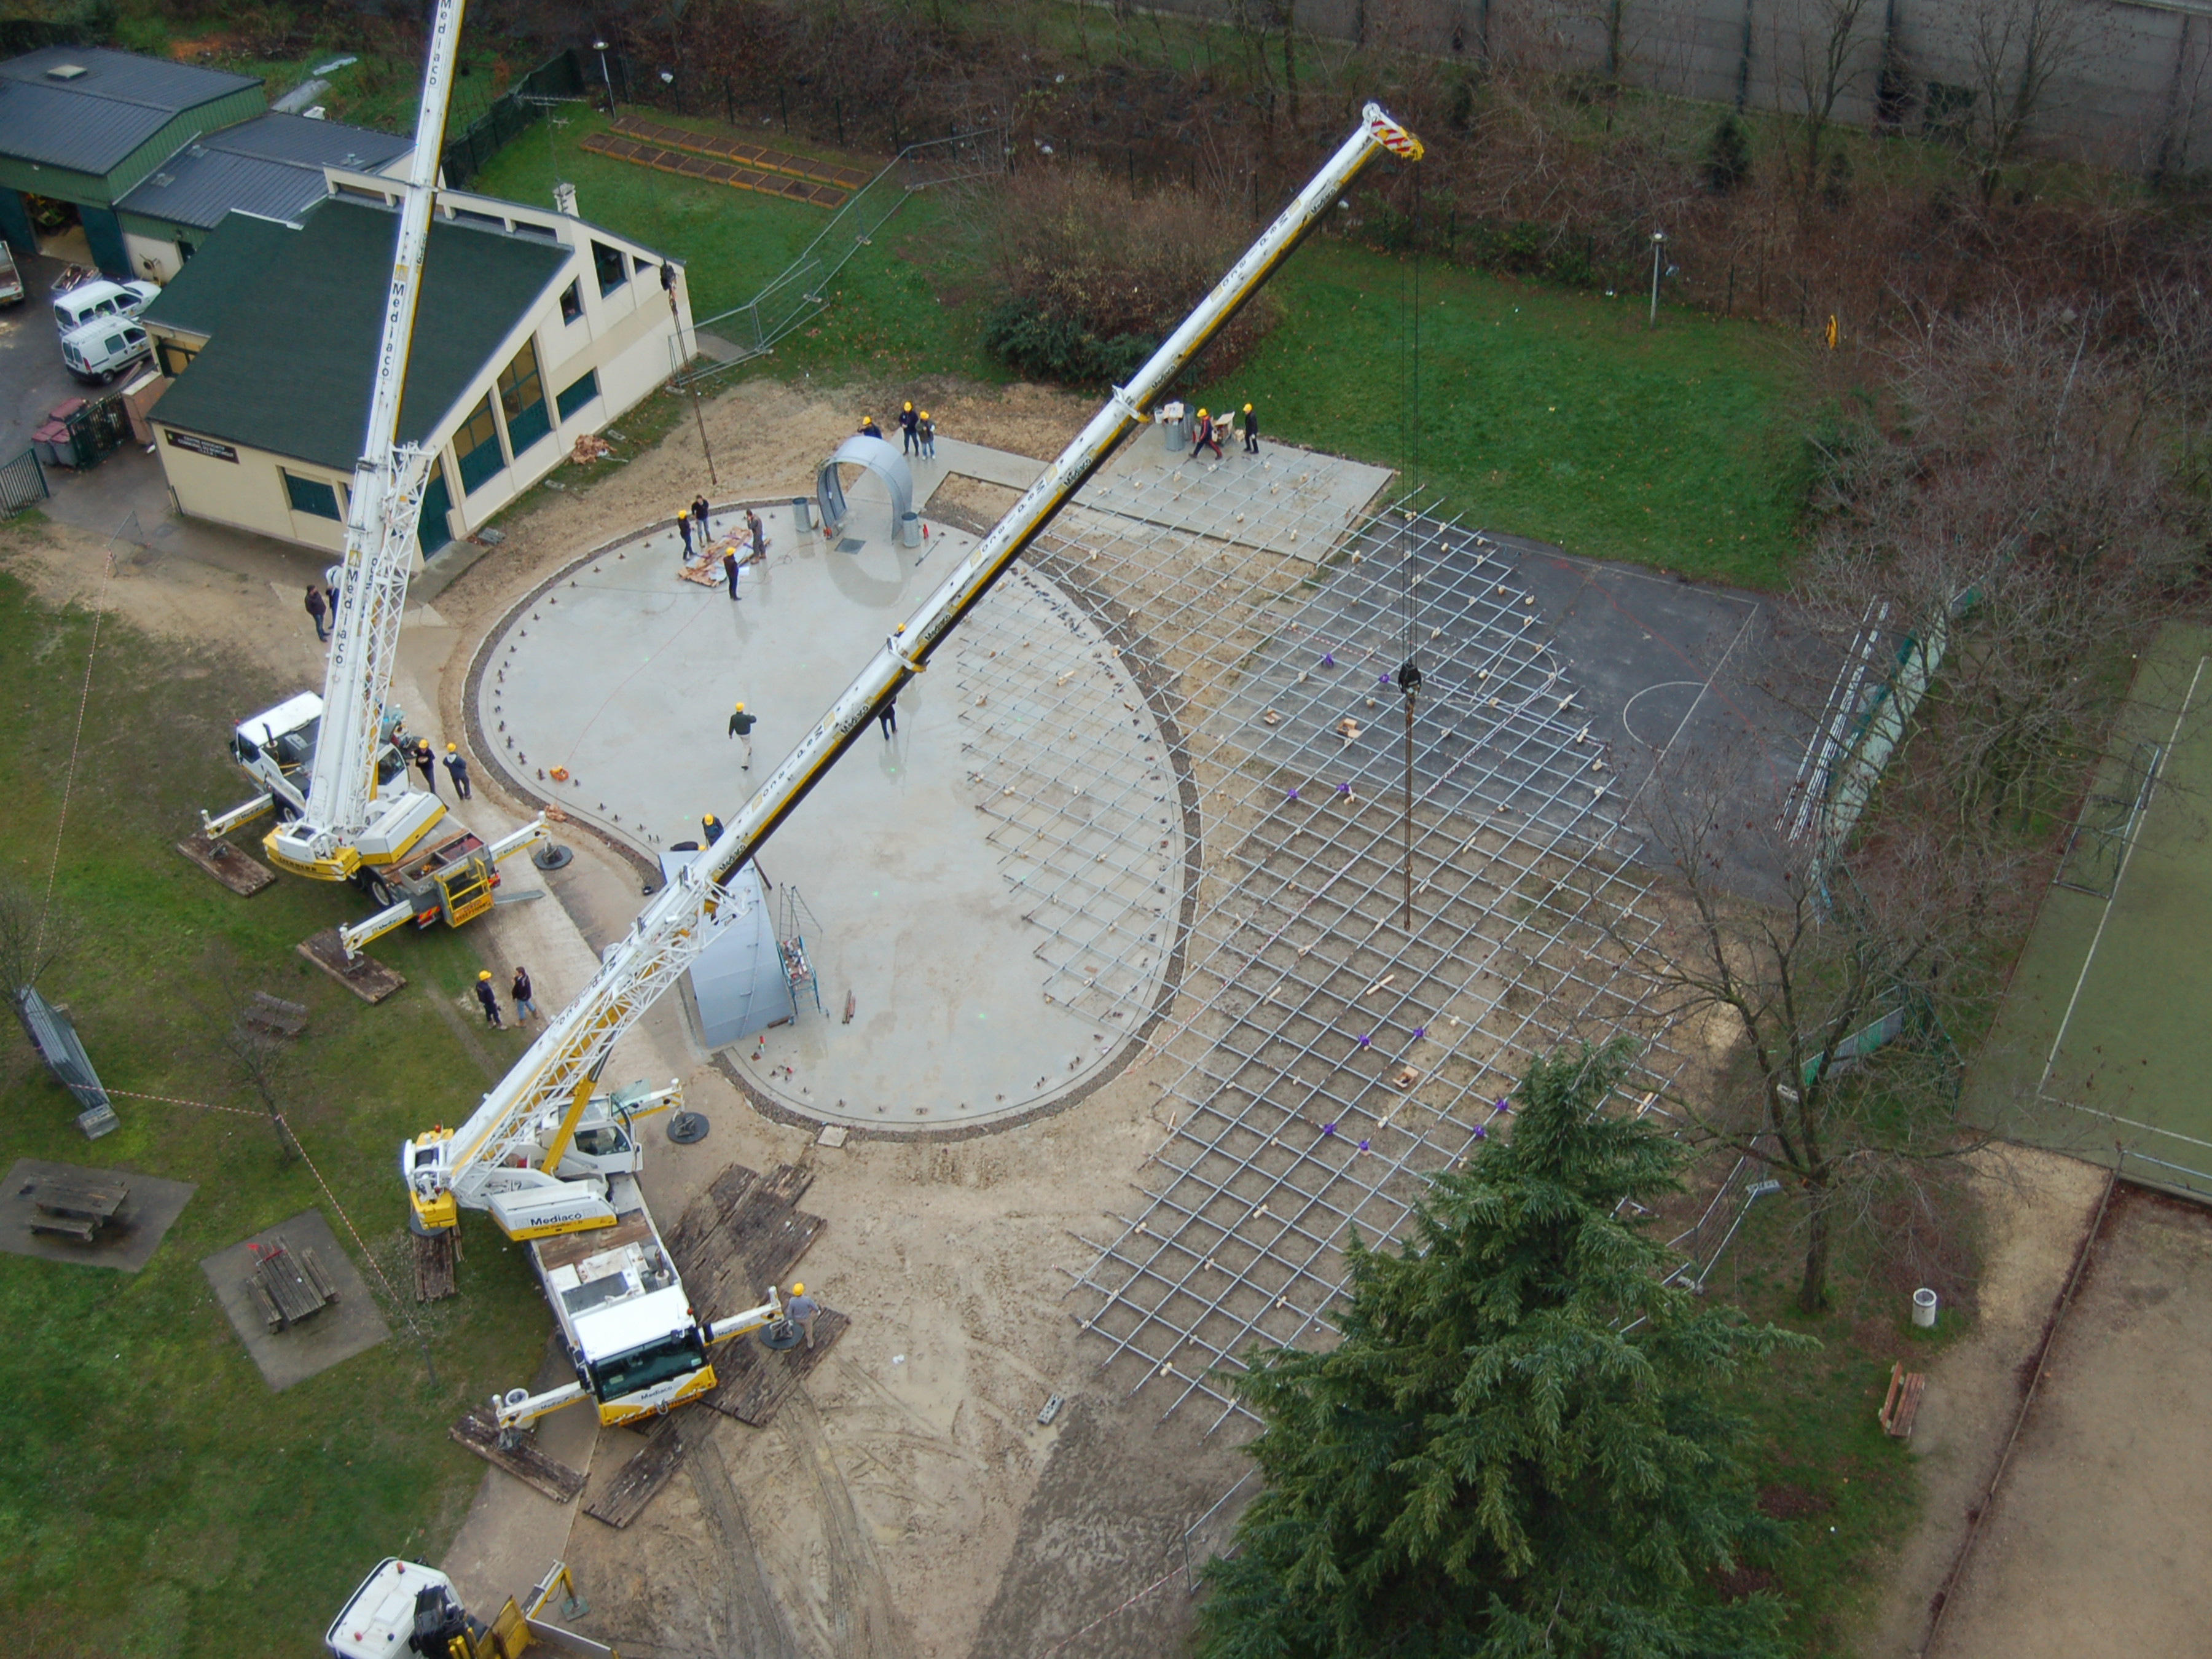
\includegraphics[width=0.48\textwidth]{cp_1.jpg}\label{fig:cp_1}}
		\hspace*{\fill}
		\subfloat[][Erection.]{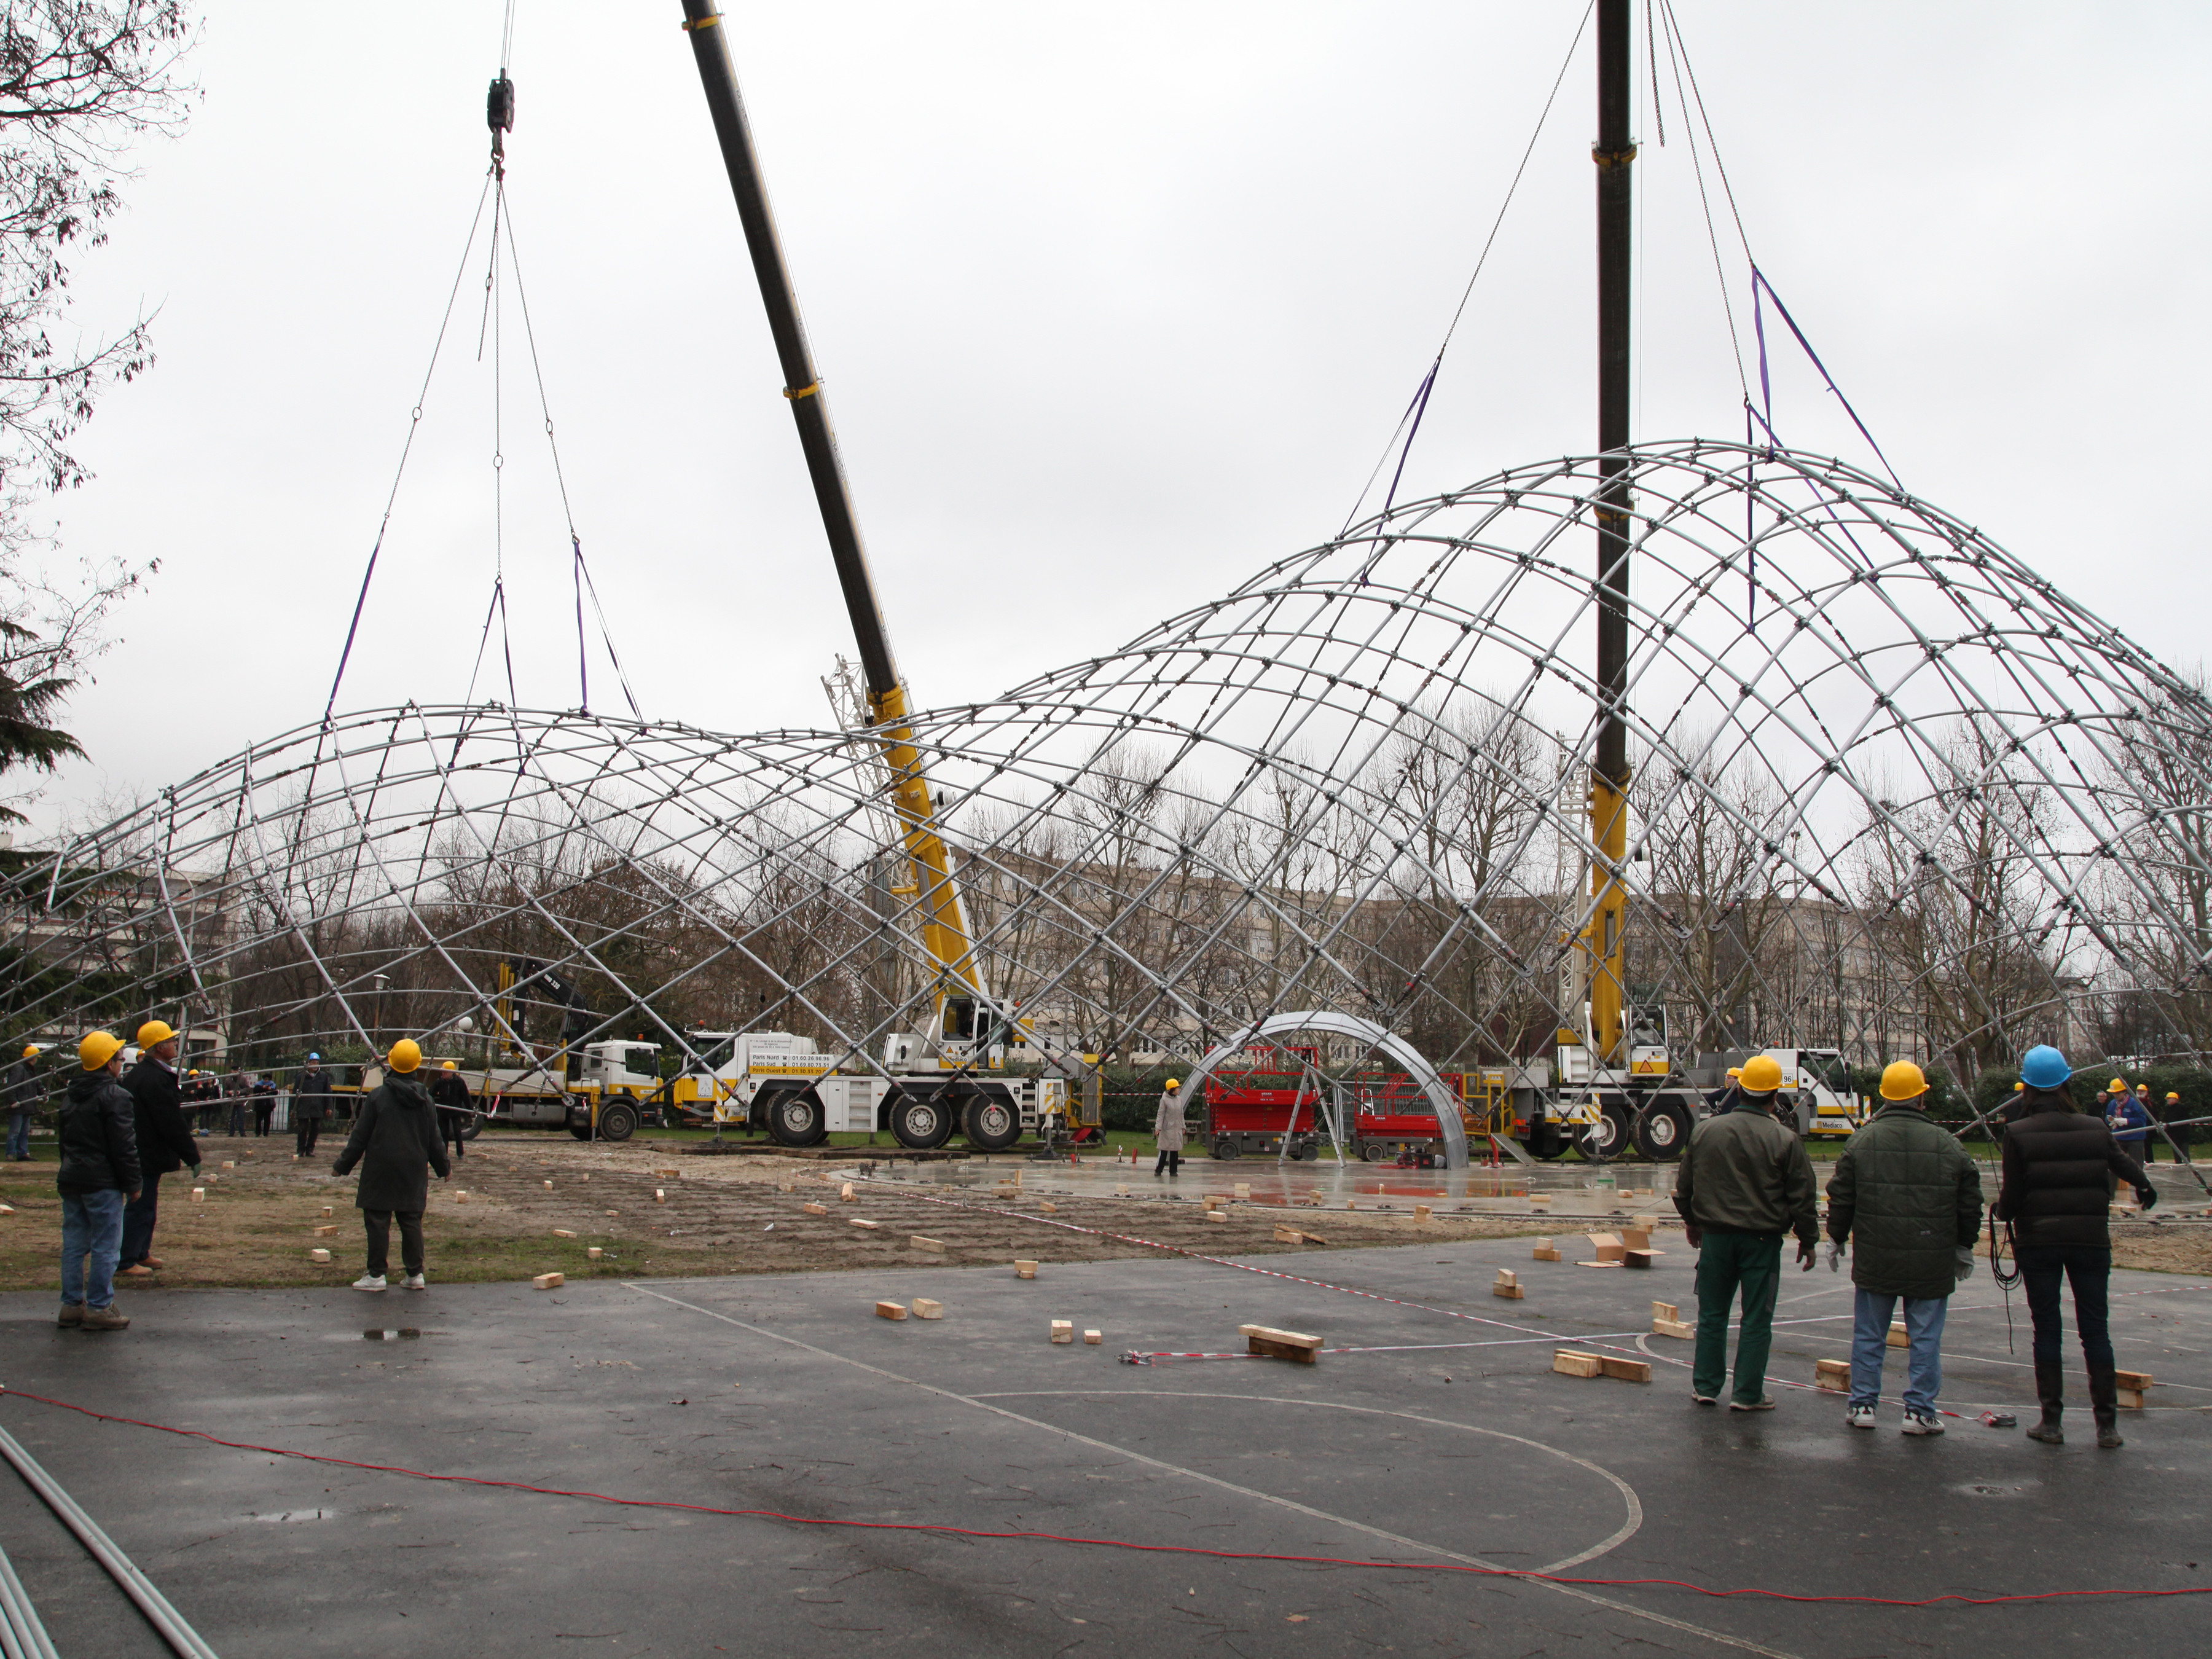
\includegraphics[width=0.48\textwidth]{cp_2.jpg}\label{fig:cp_2}} \\
		%
		\subfloat[][The grid is anchored.]{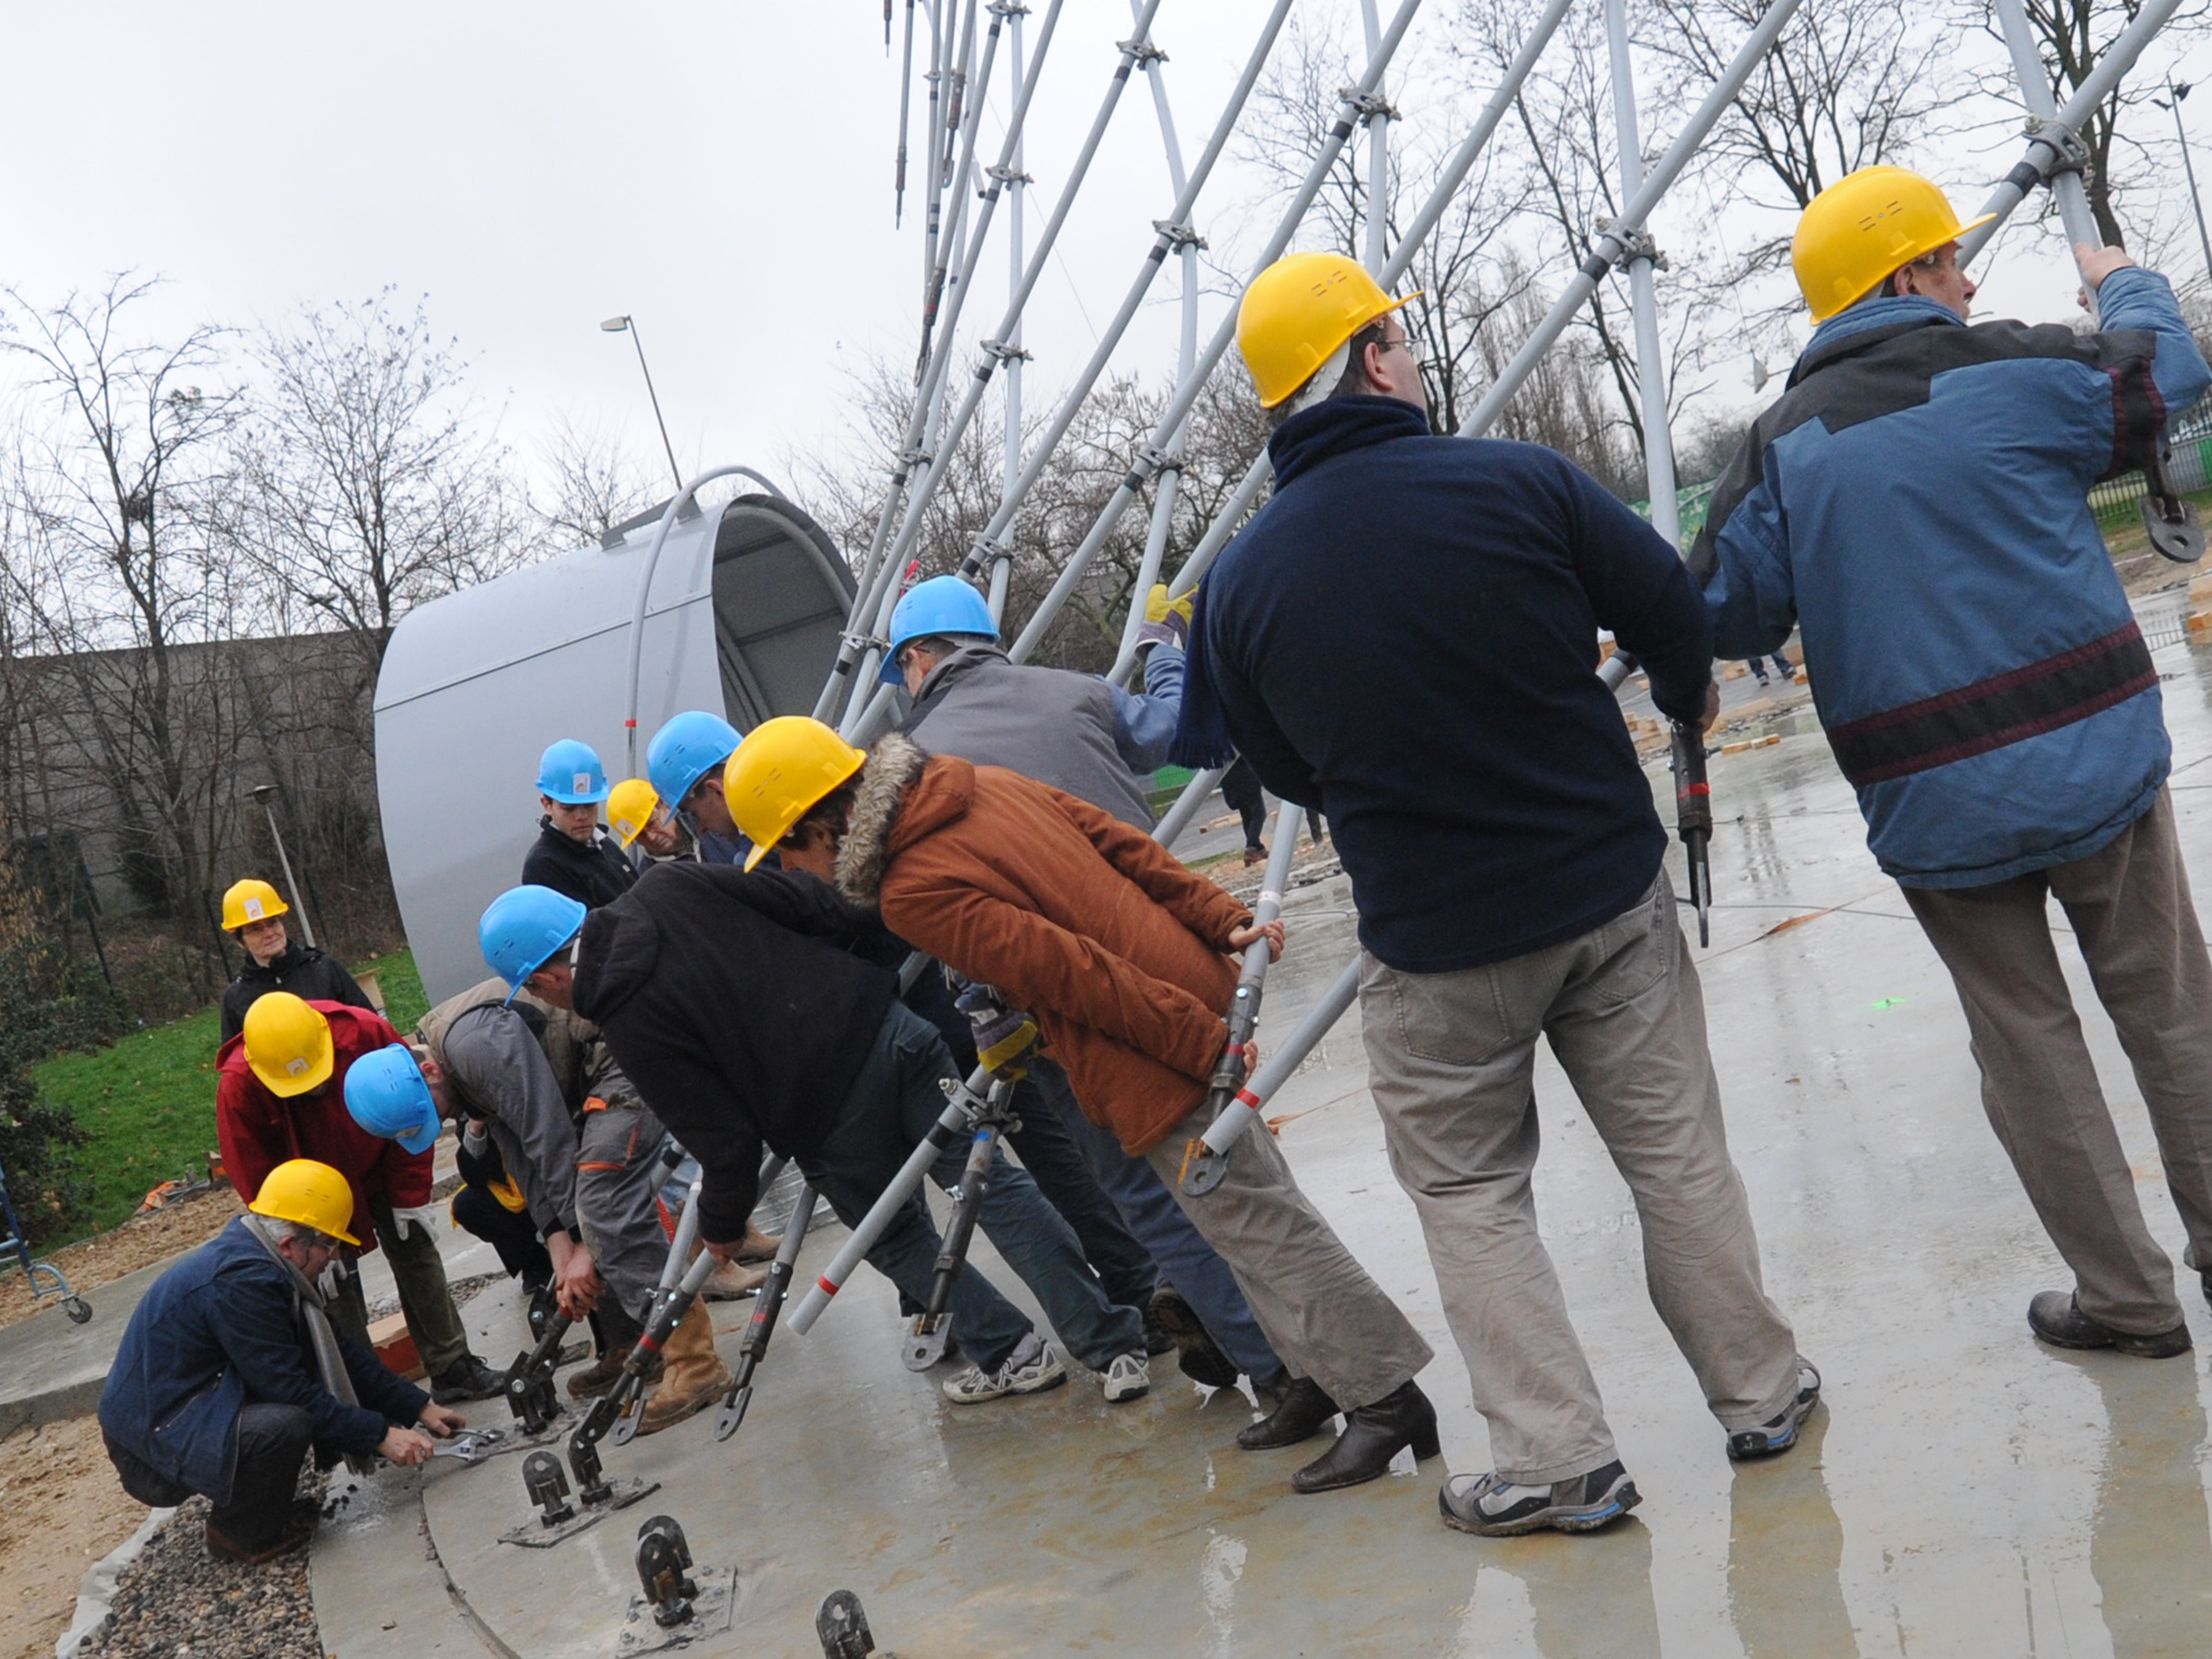
\includegraphics[width=0.48\textwidth]{cp_3.jpg}\label{fig:cp_3}}
		\hspace*{\fill}
		\subfloat[][Deformed grid.]{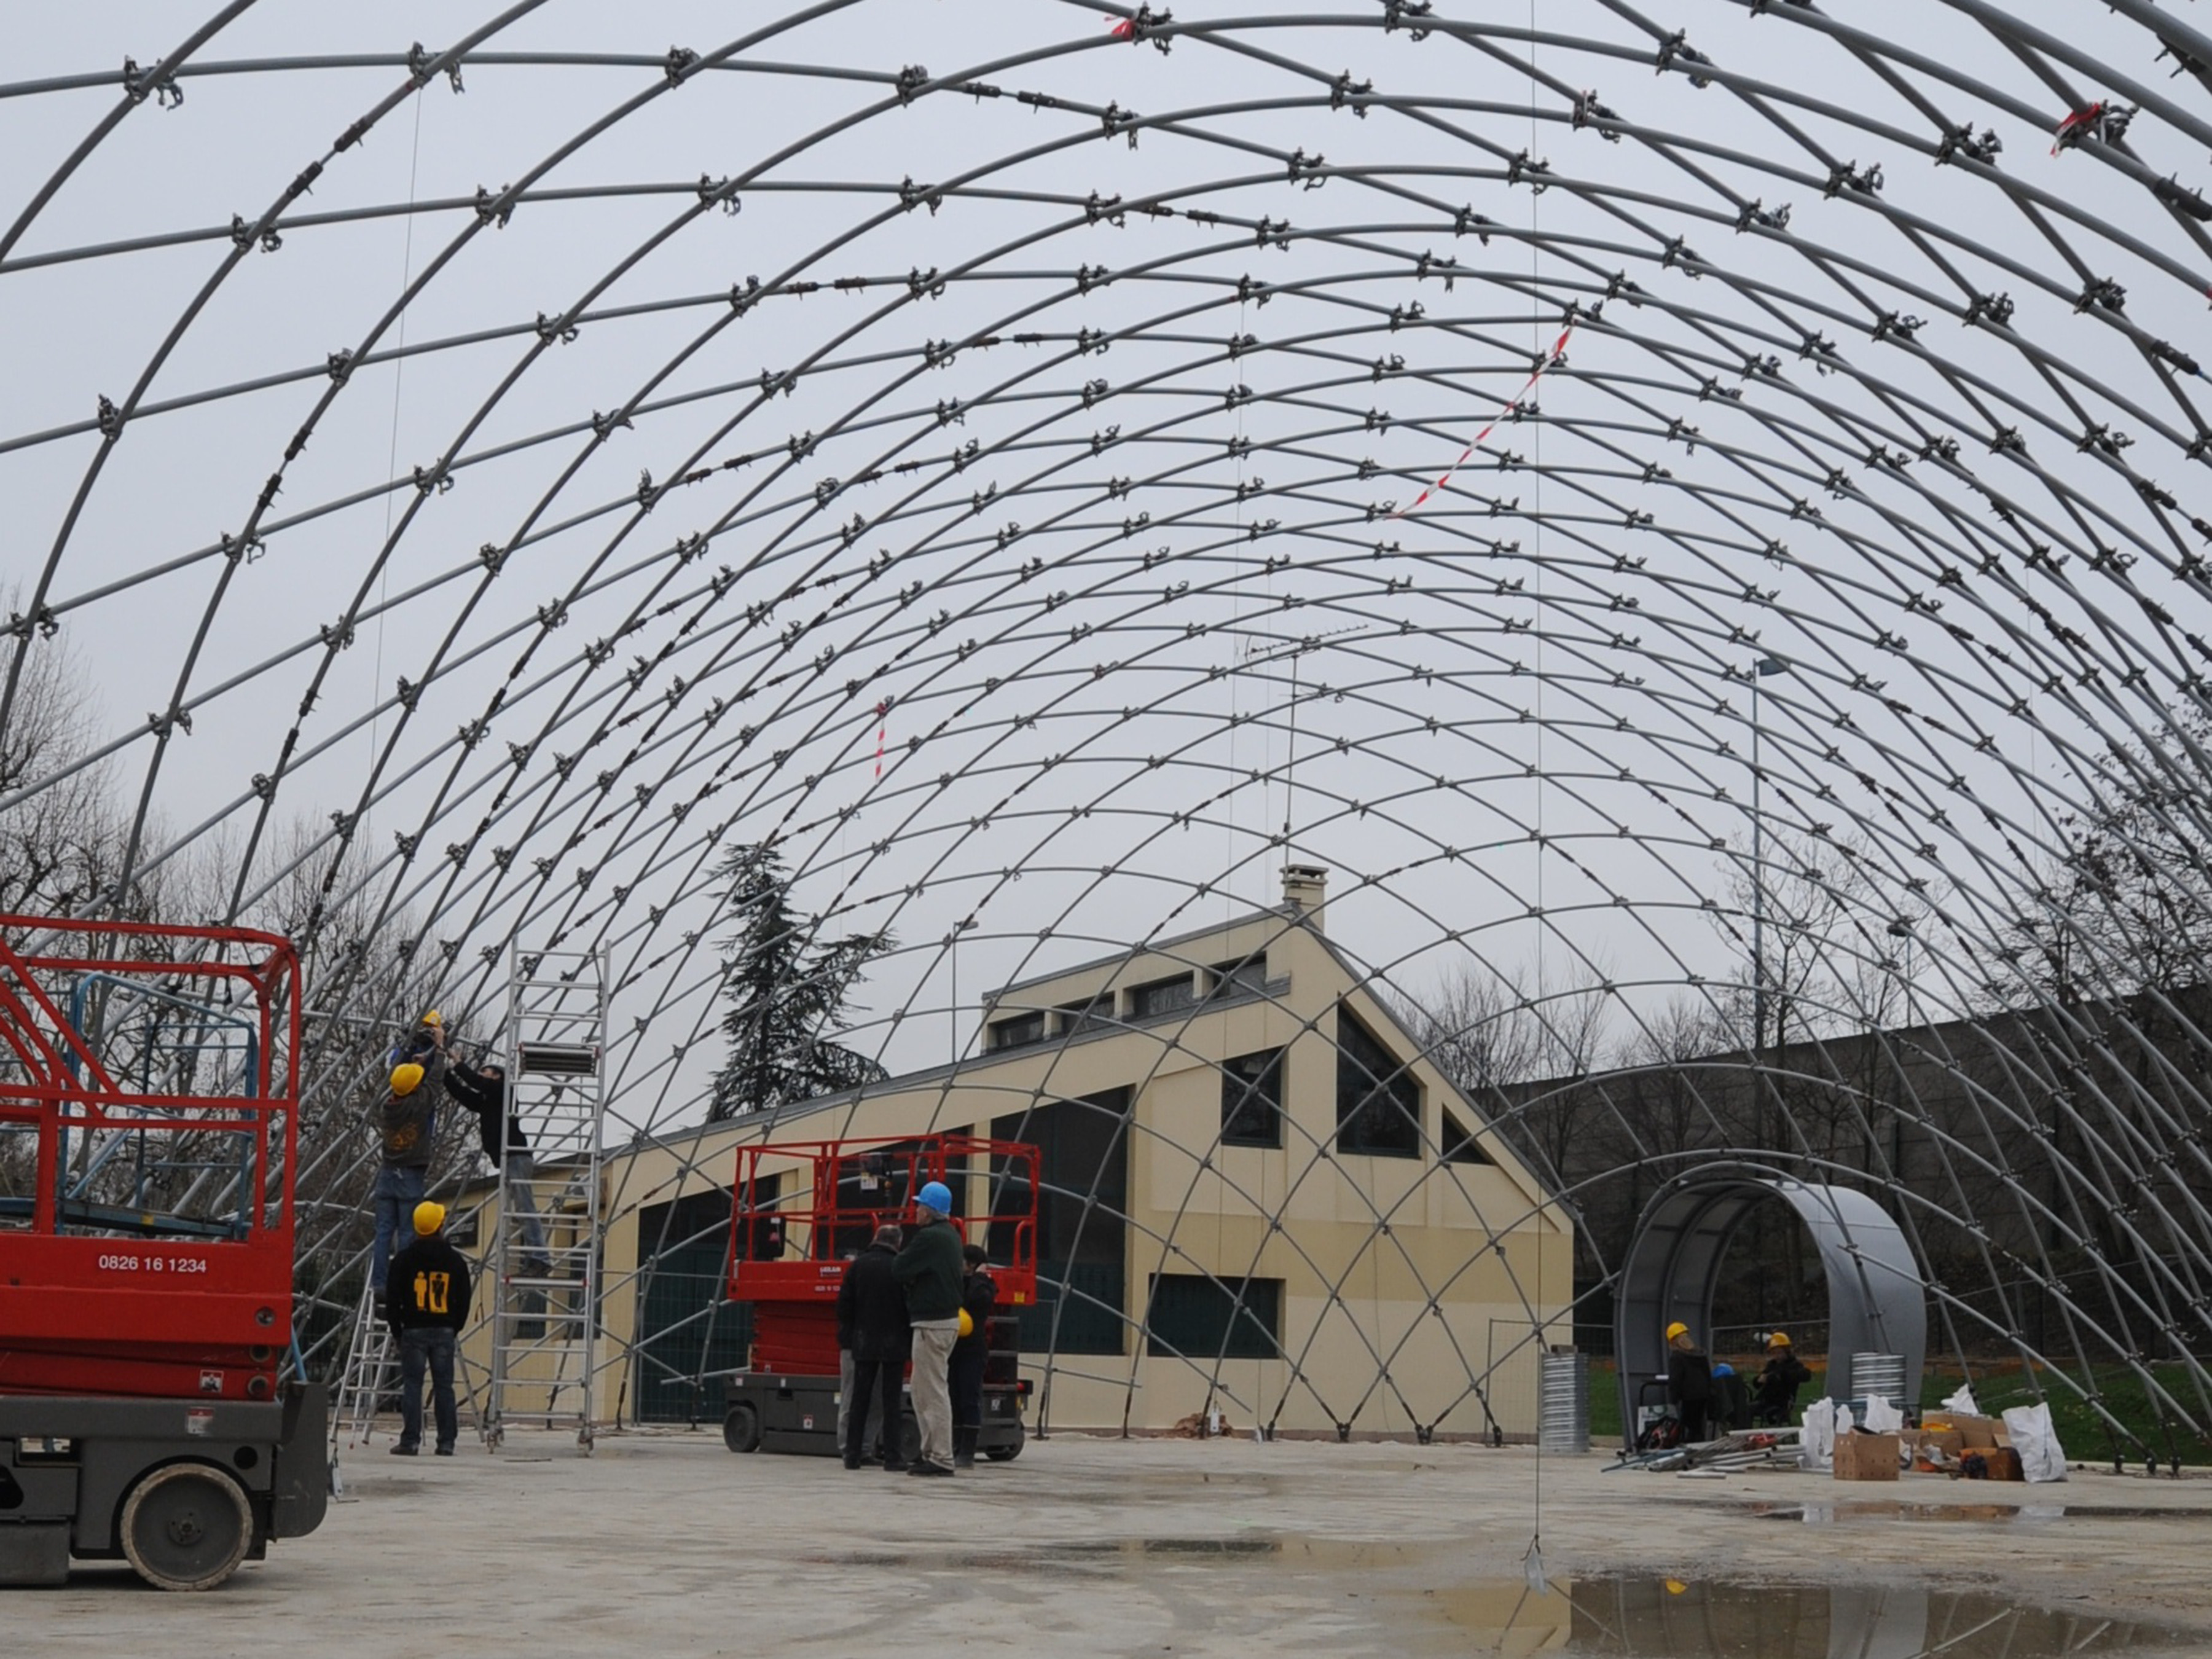
\includegraphics[width=0.48\textwidth]{cp_4.jpg}\label{fig:cp_4}} \\
		%
		\subfloat[][Grid is braced.]{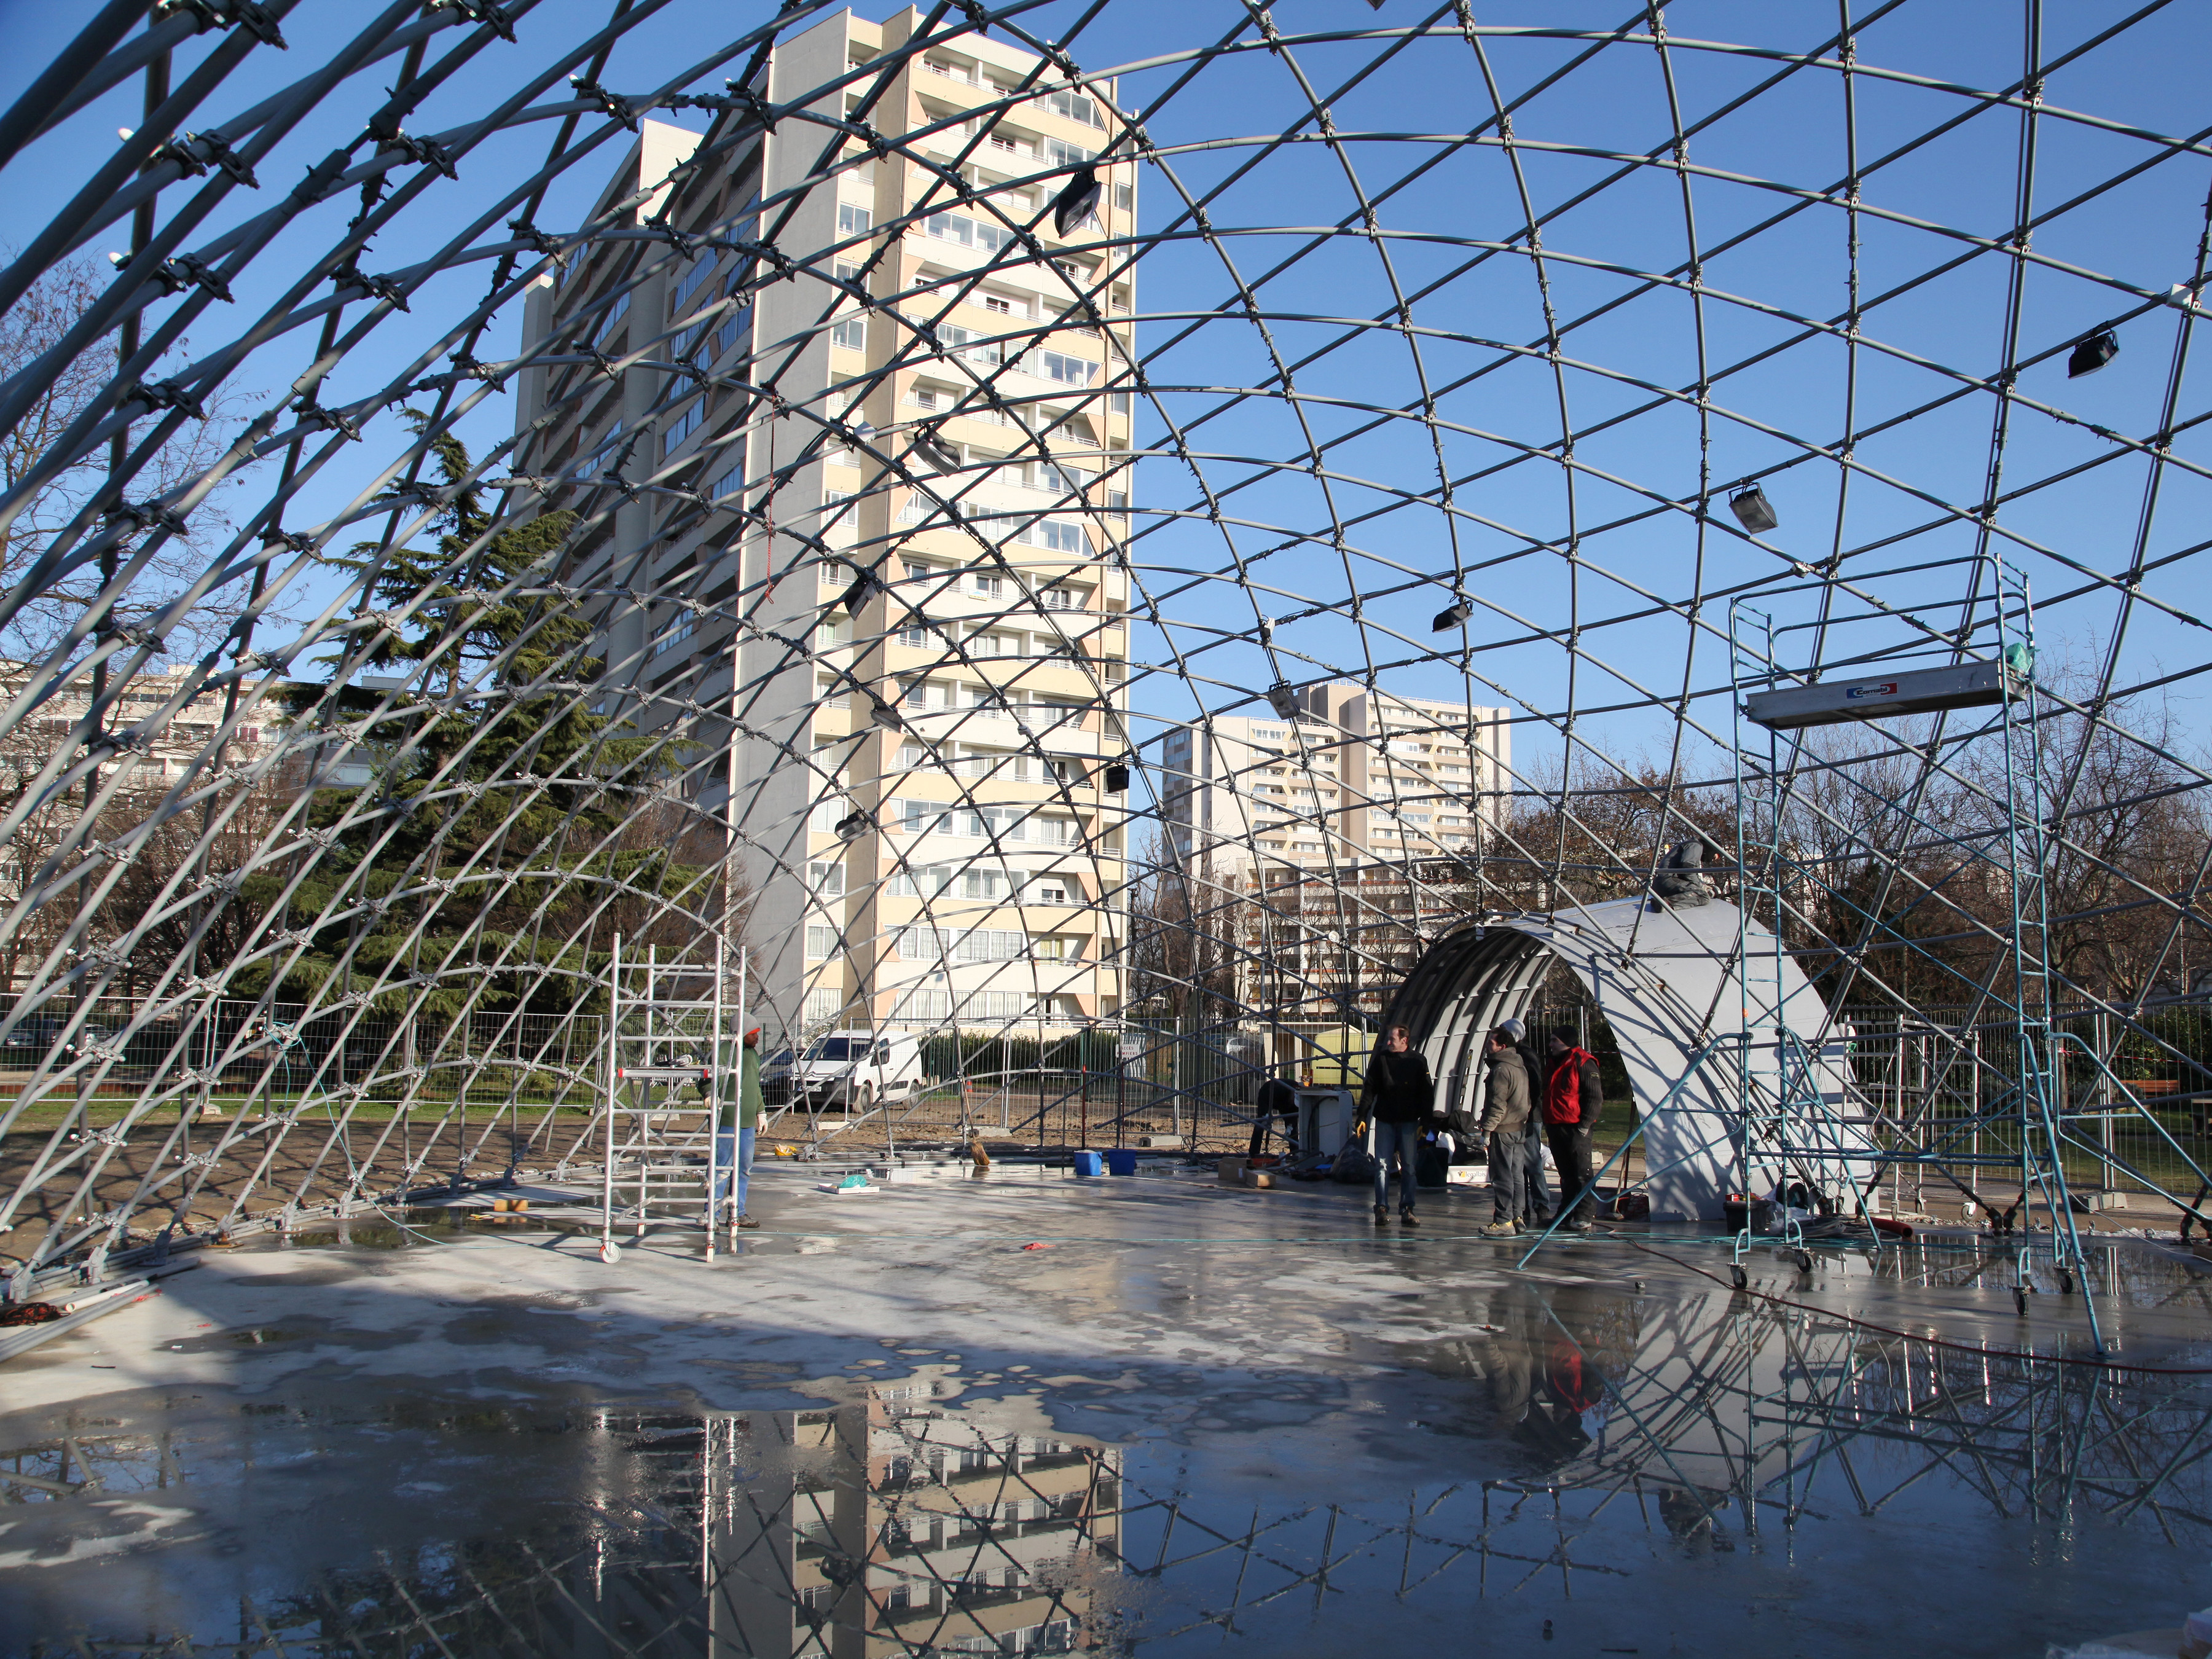
\includegraphics[width=0.48\textwidth]{cp_5.jpg}\label{fig:cp_5}}
		\hspace*{\fill}
		\subfloat[][Membrane.]{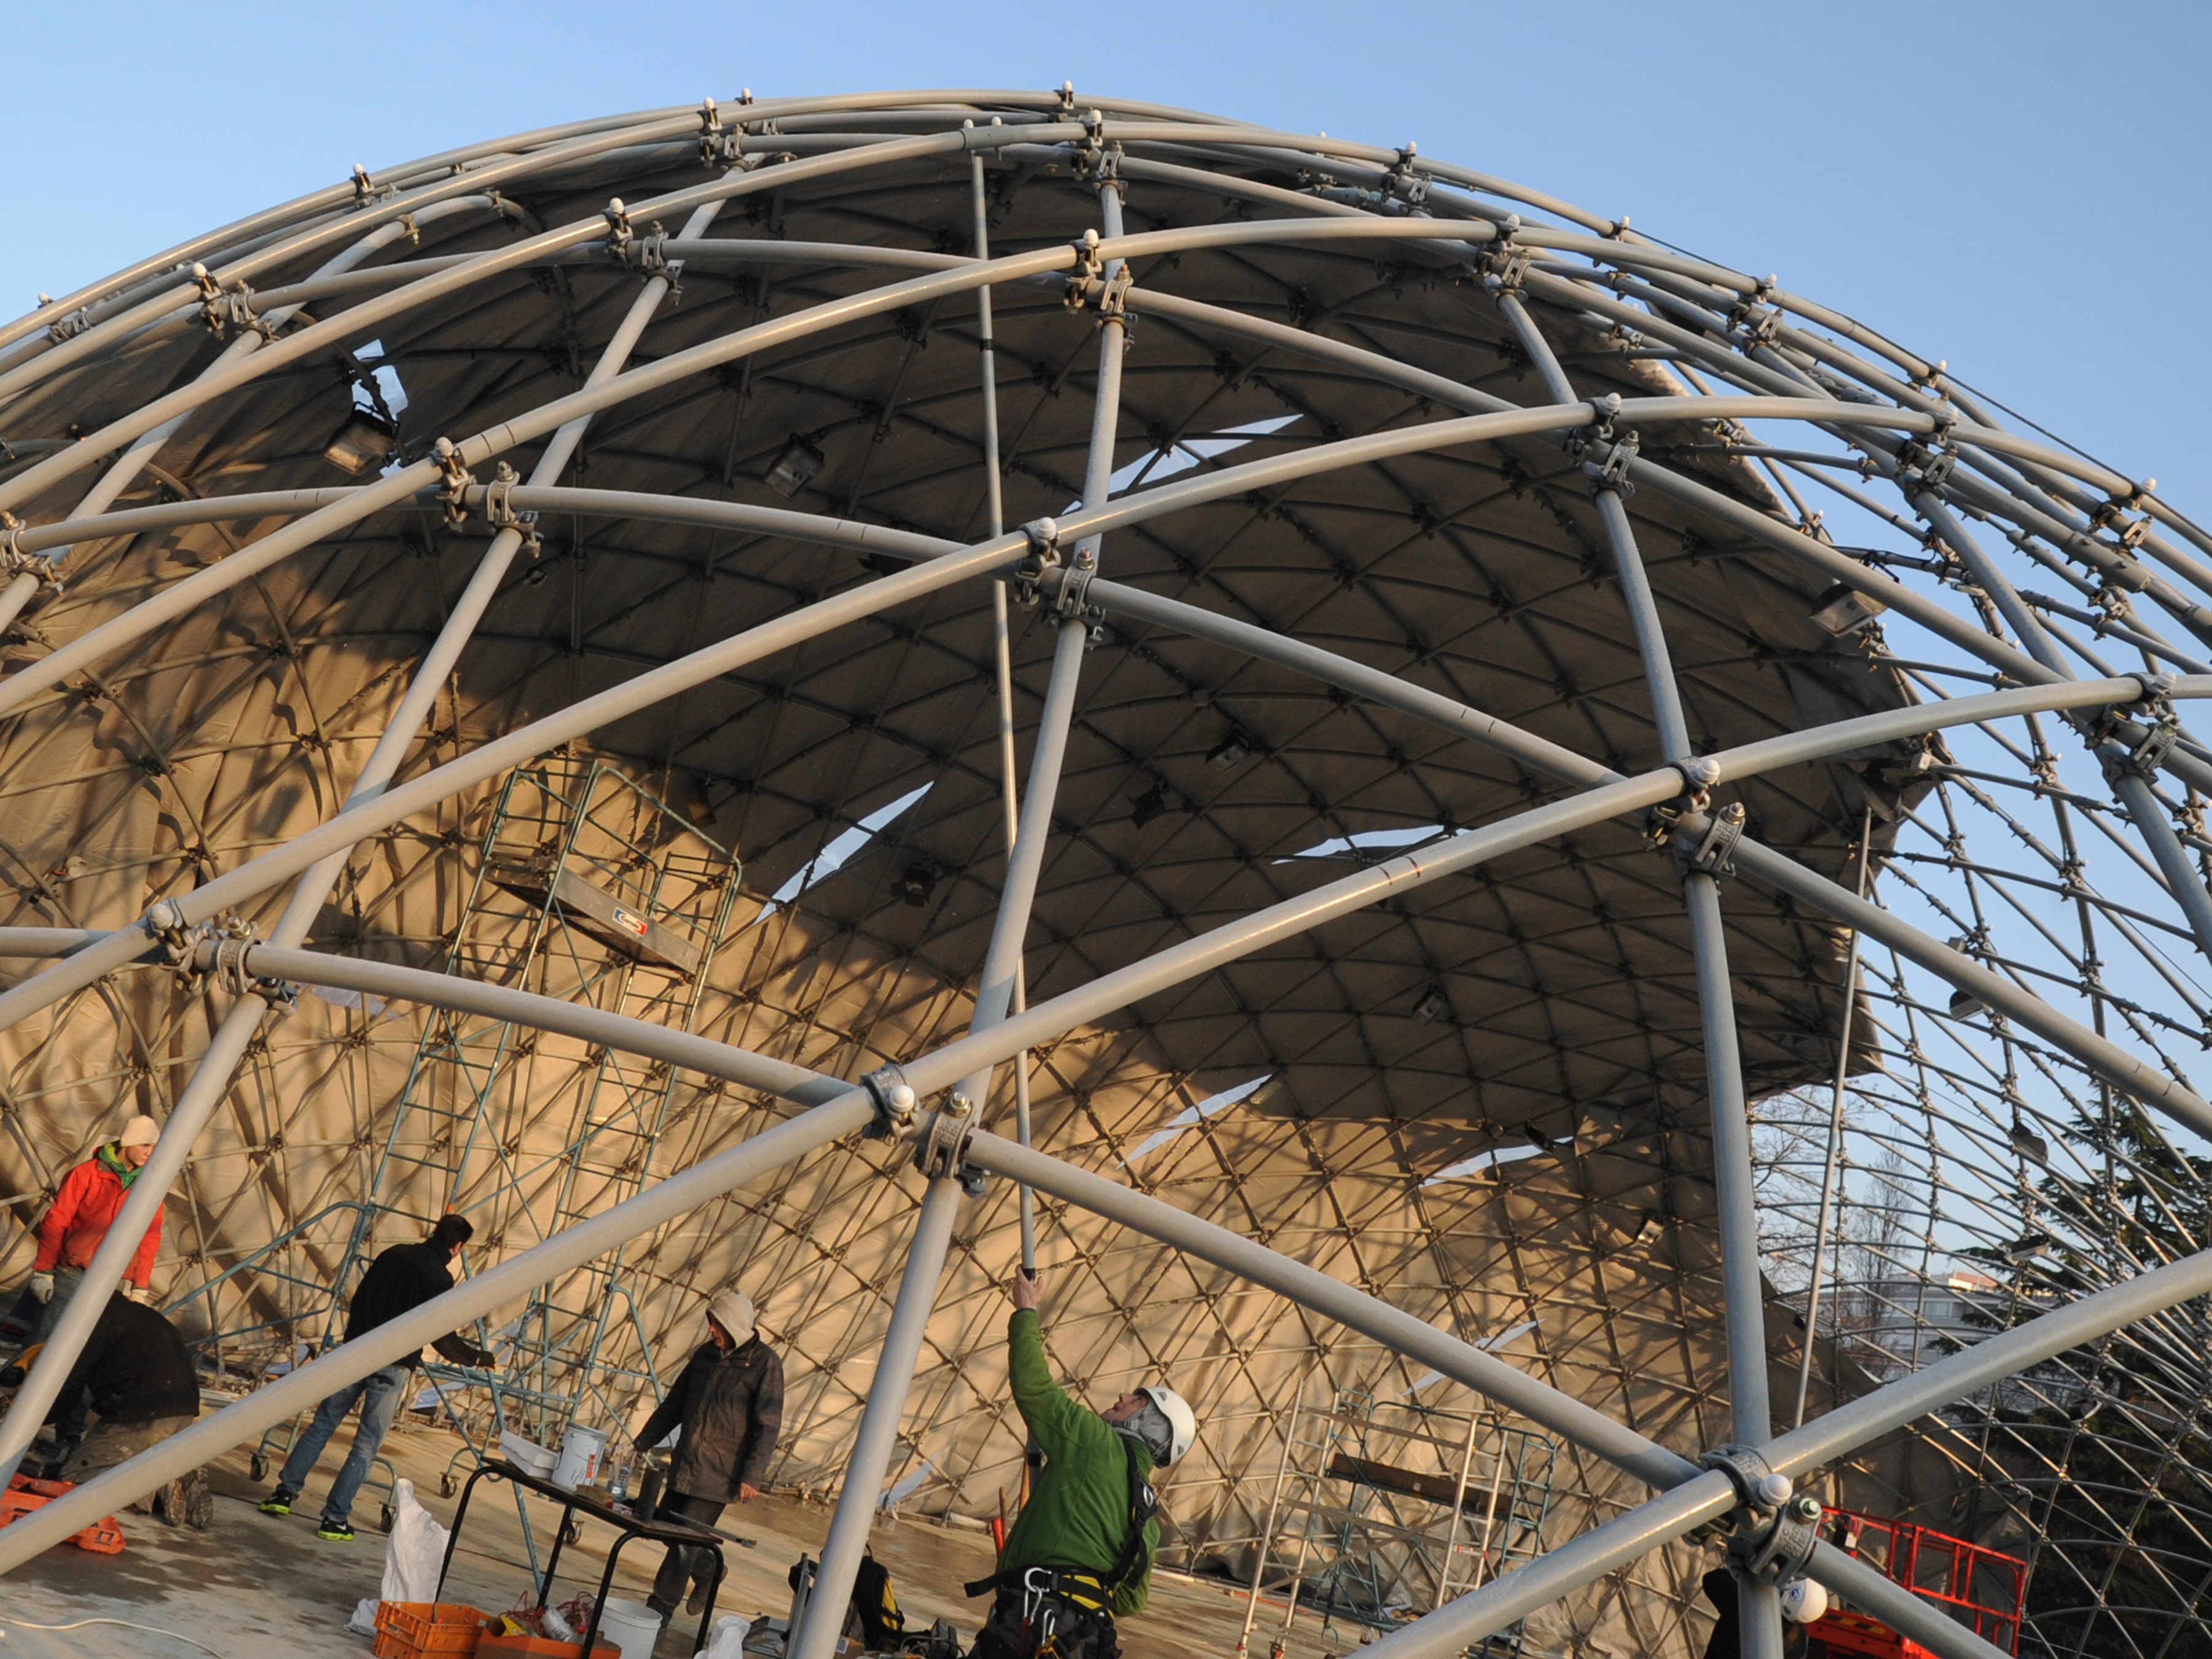
\includegraphics[width=0.48\textwidth]{cp_6.jpg}\label{fig:cp_6}} \\
		%
		\vspace{10pt}
		\caption{Construction process of the gridshell.}
		\label{fig:erection}    
	\end{fullpage}
\end{figure}

\section{Construction details}
% ====================
In this project, one can identify 4 major structural details : the swivel coupler for connecting composite tubes to assemble the grid (\autoref{fig:8}a); the steel sleeve for connecting several composite tubes to make long members from initially short piece of tubes (\autoref{fig:8}b); ground anchorages for fixing the structure to the concrete slab (\autoref{fig:8}c) and the lacing edge beam of the fabric (\autoref{fig:8}d).
Note that the tricky issue of connecting steel and composite parts is solved in a similar way through sleeve and anchorage details.

\subsection{The tubes in glass fiber reinforced polymer}
% -------------------------------------------------------


\subsection{The swivel coupler}
% -------------------------------------------------------



Tubes are connected together with scaffold swivel couplers. Each connection is composed of two collars (\O\;\SI{42}{\mm} and \SI{38}{\mm} wide) linked by a steel axis (see \cref{fig:swivel_dwg}). Thus the collars can freely rotate around the axis of the connection. This degree of freedom is responsible for the lack of in-plane shear stiffness of the primary grid and this is precisely this mechanism that allows the flat grid to deform into a free form surface.

Each collar is itself composed of two hemicylindrical parts so that it can be opened to easily engage a tube. A M12 nut and a swivel T-bolt allow to lock the tube in the collar using friction. Collars are positioned over a \SI{1.5}{\mm} thick epdm ribbon wrapped around the tubes. This layer improves the distribution of stresses generated by the transverse compression of the collar over the tube. More over, it improves the friction coefficient between the steel collar and the GFRP tube. EPDM ribbon were ordered with an adhesive side to facilitate their placement on the tubes.

Once clamped in the connection, the tubes are spaced by a \SI{68}{\mm} distance from axis to axis. Although the mechanical consequences of this eccentricity could be neglected to a first-order approximation, this is not the case for the geometric consequences it induces as explained in \cref{sec:asbuilt}.

This connection has the advantage to be available almost every where, to be really cheap and almost indestructible compare to the GFRP members. However, there are some drawbacks as it is not tailor-made for the purpose of elastic gridshells in composite materials :
\begin{itemize}
\item Firstly, the weight of this part is about \SI{1}{\kg}, which is very heavy compare to the lightness of the system. In this project, the weight of the swivel couplers represent one third of the overall weight of the structure. This could easily be reduced with a dedicated design.
\item Secondly, this part is made for assembling scaffolds where workers should tight strongly the collars of the coupler to ensure that the steel tubes won't slide in their collar. Here this is clearly not possible. Indeed the GFRP tube is to thin (only \SI{3.5}{\mm} thick) and tightening the collars to the maximum would damage it.
\end{itemize}

\begin{figure}[p]
	\begin{fullpage}
	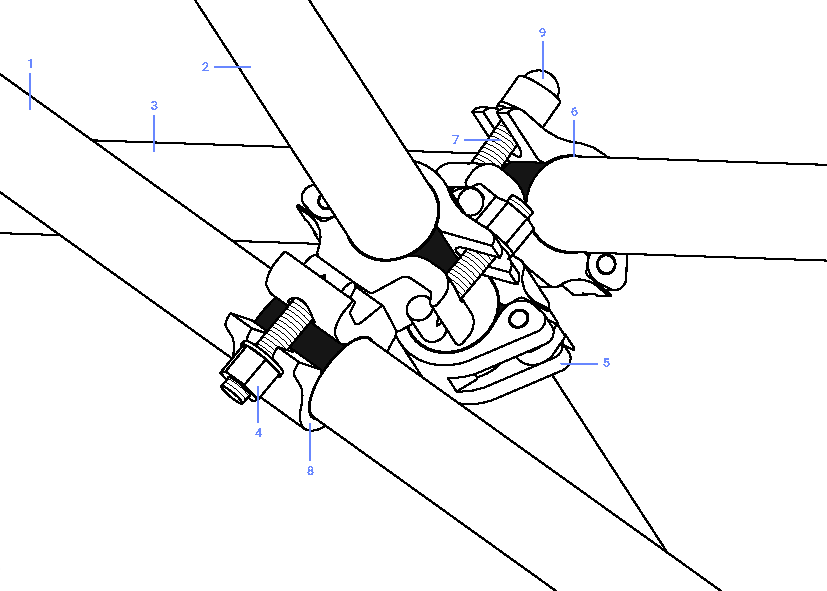
\includegraphics[width=1\textwidth]{swivel.pdf}
	\caption{Technical drawing of the swivel coupler. GFRP tubes (1, 2, 3). Swivel couplers (5, 8). EPDM layer (6). M12 swivel T-bolt (7). M12 nut (4) and plastic cap (9).}
	\label{fig:swivel_dwg}
	\vspace{1cm}
	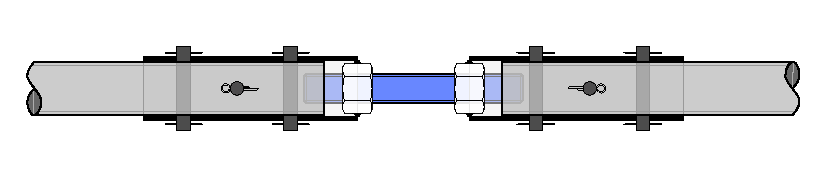
\includegraphics[width=1\textwidth]{sleeve.pdf}
	\caption{Technical drawing of the sleeve system.}
	\label{fig:sleeve_dwg}
	\end{fullpage}
\end{figure}


\begin{figure}[ht]
\centering
\begin{fullpage}
	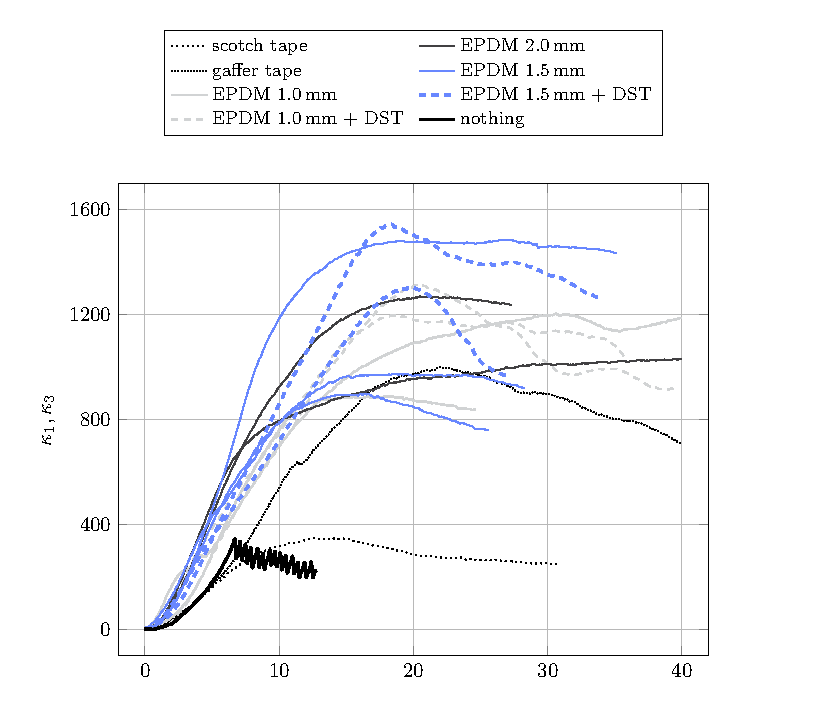
\includegraphics[]{ch2a_creteil/plot/1_layer_benchmark/build.pdf}\label{plot:layer_benchmark}
	\caption{Influence of the interface layer on the sliding resistance.}
\end{fullpage}
\end{figure}

\begin{figure}[ht]
\centering
\begin{fullpage}
	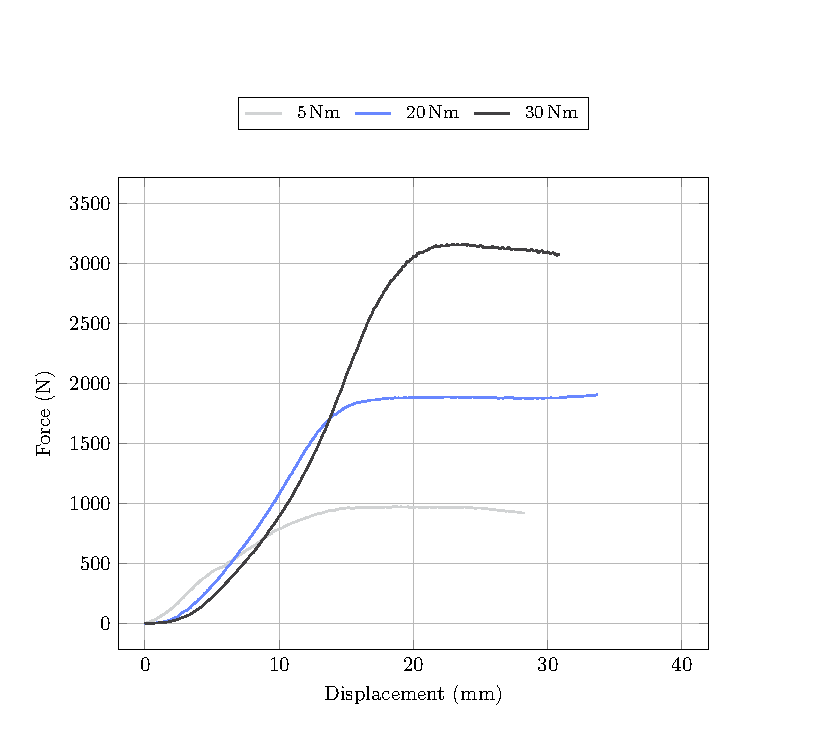
\includegraphics[]{ch2a_creteil/plot/3_tightening/build.pdf}\label{plot:tightening}
	\caption{Influence of the tightening on the sliding resistance.}
\end{fullpage}
\end{figure}

\begin{figure}[ht]
\centering
\begin{fullpage}
	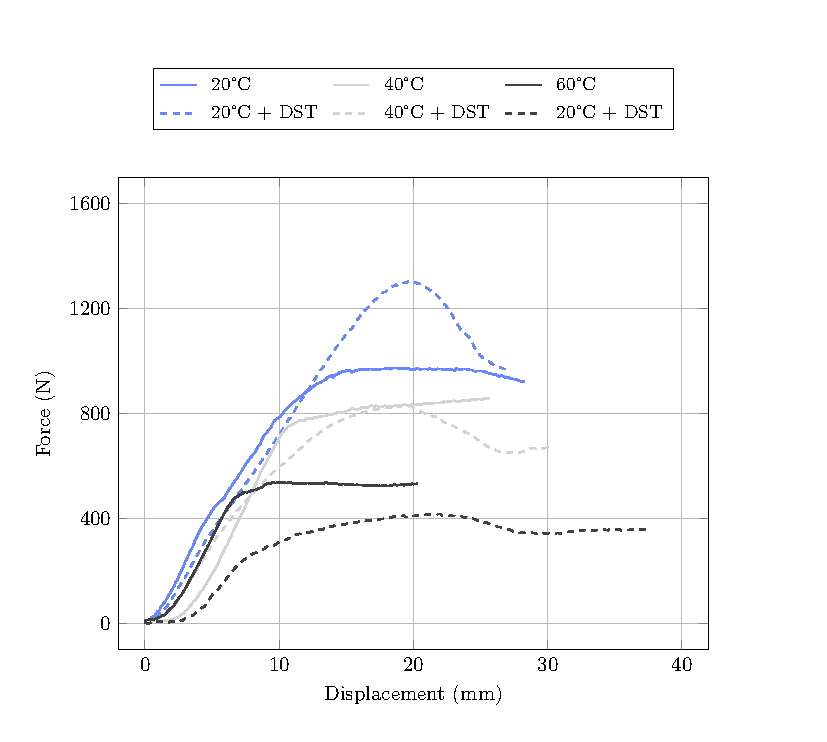
\includegraphics[]{ch2a_creteil/plot/2_epdm_temperature/build.pdf}
	\caption{Influence of the temperature on the sliding for a \SI{1.5}{\mm} EPDM layer.}
	\label{plot:epdm_temperature}
\end{fullpage}
\end{figure}

\begin{figure}[ht]
\centering
\begin{fullpage}
	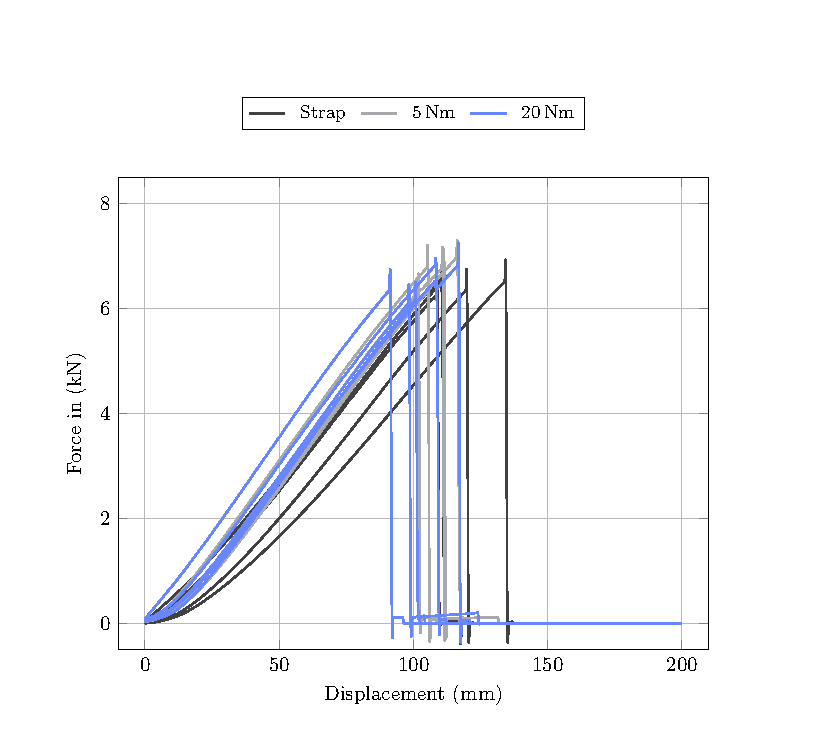
\includegraphics[]{ch2a_creteil/plot/4_gfrp_tube/build.pdf}
	\caption{Flexural tests of the GFRP tubes.}
	\label{plot:epdm_temperature}
\end{fullpage}
\end{figure}

\subsection{The sleeve system}
%------------------------------------------

\subsection{Concrete footing}
%------------------------------------------


\section{Design Process}
%=================

\subsection{Overall design process}
%------------------------------------------

The goal of the design process is to identify a gridshell structure that works and respects as faithfully as possible the architectural project – a shape and a program. It represents “the path from shape to structure”. Its progress, sequential and iterative, revolves around three major stages: shape, mesh and structure. It is not trivial to go through this complex process. Indeed, for each step, the method, the tool, the criteria, that offers both a sufficient explorative richness to find out enough candidate solutions, and the means to evaluate and compare the suitability of those solutions, have to be found.
\begin{figure}[t]
\centering
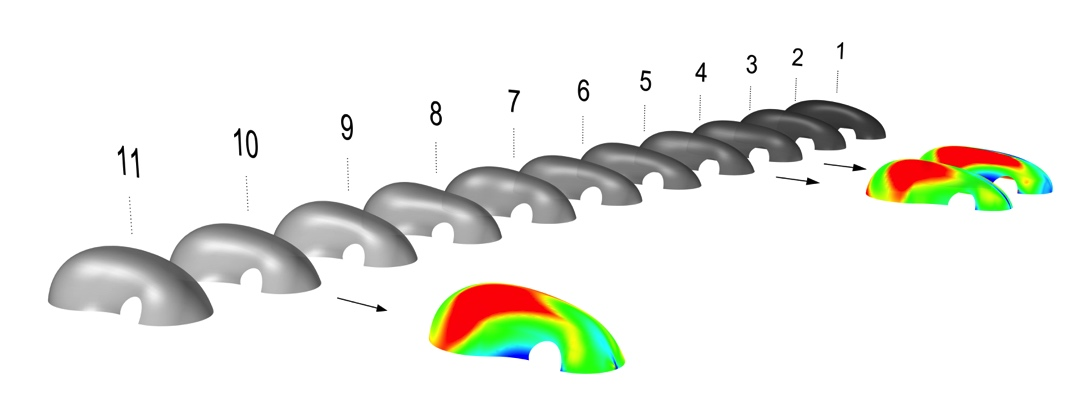
\includegraphics[width=\textwidth]{image8}
\caption{Evaluating the mechanical potential of shapes regarding principal curvatures}
\label{fig:7}
\end{figure}

\subsection{3D modelling of the intended shape}
%------------------------------------------
The first step of the process consists in building a precise geometric model from the sketch of the architect and to evaluate its mechanical potential (\autoref{fig:7}). At this stage, the goal is to estimate the probability a given shape would lead to the generation of a structurally feasible gridshell.

Stresses in the grid are mainly due to the bending of the profiles. They derive directly from their geometric curvature. Thus, the principal curvatures of the surface – because they give a qualitative measurement of the local curvature of any curve drawn on a surface – are relevant indicators to evaluate the stress rate of a grid laying on it. Particularly, one should ensure the following condition is satisfied everywhere, where $r$ is the pipe’s outer radius, $R_{min}$ is the minimum principal radius, E is the flexural modulus, $\sigma_{k,flex}$ the characteristic flexural strength and $\gamma_{lt}$ the long-term partial coefficient of material resistance :
\begin{equation}
	\mathrm{E} = \frac{r}{R_{min}} < \frac{\sigma_{k,flex}}{\gamma_{lt}} 
\end{equation}

Ideally, the shape is controlled by few key parameters. Thus, it can be adapted and optimized through an iterative process, towards this criterion.

\subsection{Mesh from the compass method}
%------------------------------------------
During the second step, the candidate surface is meshed and the mechanical potential of the resulting grid is evaluated. At this stage, we try to estimate the probability a given mesh could lead to the generation of a viable gridshell structure. Simultaneously, meshes are compared according to their architectural relevance.

This time, the geometric curvature of the polylines drawn on the surface is the criterion to characterize the mechanical potential of the grid. In particular, one should ensure the following condition is satisfied everywhere, where $R_{spline}$ is the spline’s local curvature radius :
\begin{equation}
\mathrm{E} =  \frac{r}{R_{spline}}  <   \frac{\sigma_{k,flex}}{\gamma_{lt}}
\end{equation}

The mesh is obtained by the compass method, described in \citep{Otto1974}, which develops a regularly spaced grid on a surface from two secant directrix. For a given shape there are an infinite number of meshes. The aim is to identify at least one grid, suitable towards architectural and structural criteria. The laboratory tried various numerical methods to generate such grids \citep{Bouhaya2009}. Here, a specific software \citep{DuPeloux2011}, developed for rhino \& grasshopper, allows generating this kind of mesh on any NURBS surface.


\subsection{Formfinding and bending prestress}
%------------------------------------------
From now on, the initial form has been optimized and promising meshes for the materialization of the future gridshell have been identified. However, they do not take account of any true mechanical reality, because only geometric rules have led to their generation. The formfinding step consists precisely in finding the geometry of the grid at mechanical equilibrium, and the corresponding permanent bending stresses.
The calculations, performed numerically thanks to a dynamic relaxation algorithm with kinetic damping \citep{Barnes1975}, is composed of the following steps:
\begin{enumerate}
\item The grid is bent by a set of applied displacements from rest to compass position
\item The grid is then relaxed through its mechanical equilibrium
\item Bending stresses of the triangulation are calculated relative to the relaxed geometry
\item Geometry and bending stresses of the triangulation are reinjected in the model
\end{enumerate}

Two analysis models are built during this process to study the structure with or without bracing tubes.
Note that the algorithm has been improved to take account for the eccentricity due to connections \citep{Douthe2006}.

\subsection{As-built geometry}\label{sec:asbuilt}
 %-------------------------------------
Indeed, the eccentricity remains small compared with the span of the shell, but it is not negligible compared with the mesh size ($e = \SI{68}{\mm} $; l =17 m; w = 1 m). Thus, the pipe lengths and anchorage positions could not be determined with sufficient accuracy without taking into account the thickness of the structural grid due to this eccentricity. The employed method, purely geometrical, assessed that the neutral fibre of the shell is equidistant from the first two layers of pipes. The form-finding was performed only with those two layers. Connection axes had to be parallel to the local normal of the shell surface. This assumption was not exact, but, in this case, gave sufficient accuracy. The red pipe was offset by e/2, the green by e/2 and the blue by 3e/2 along the normal.

\subsection{Structural analysis}
%------------------------------------------
A full structural analysis is performed on the gridshell, using the two mechanical models created previously during the formfinding stage.
The non-braced model is used to check the grid’s behavior during the construction stages. In particular, it must be verified that the primary grid - the one with no triangulation tubes - has no risk of buckling, both for obvious safety reasons and to ensure the accuracy of the final geometry. Indeed, the more the form is likely to buckle, the more it can be triangulated in a buckled geometry different to the targeted geometry. The model with the triangulated grid is used to confirm the gridshell complies with all the structural requirements during its lifetime. Its behavior under standard loadings is evaluated.




\section{Codes for composite materials}
%------------------------------------------

Beyond the technical difficulties related to both design and structural analysis of the shell, the regulatory framework was a vital issue for the project’s success. Because it was the first time a structure of this kind would host regularly a large number of people in a long-term period, the question of its reliability over time was a major issue. To be built the gridshell had to comply with existing standards, which do not take into account such an innovative edifice, all in composite material. The strategy adopted to bypass this obstacle consisted in making the most of the existing regulatory framework to justify the compliance of a structure that would not, at first sight, be taken into account by standards that does not include composite materials.
As far as possible, the design was led in compliance with the Eurocodes, where the structural design is made according to limit states under normalized loadings (self-weight, snow, wind, etc.). Despite the Eurocodes do not directly take into account composite materials, they propose some probabilistic methods to introduce new materials (Annexe D). As far as possible, the mechanical properties of the GFRP pipe were determined by tests in conformance with these methods. Otherwise, values where taken according to the Eurocomp \citep{Clarke2003}.  In some cases, as the sleeve, the design of the construction details has also benefited from this approach.

\begin{figure}[t]
	\centering
		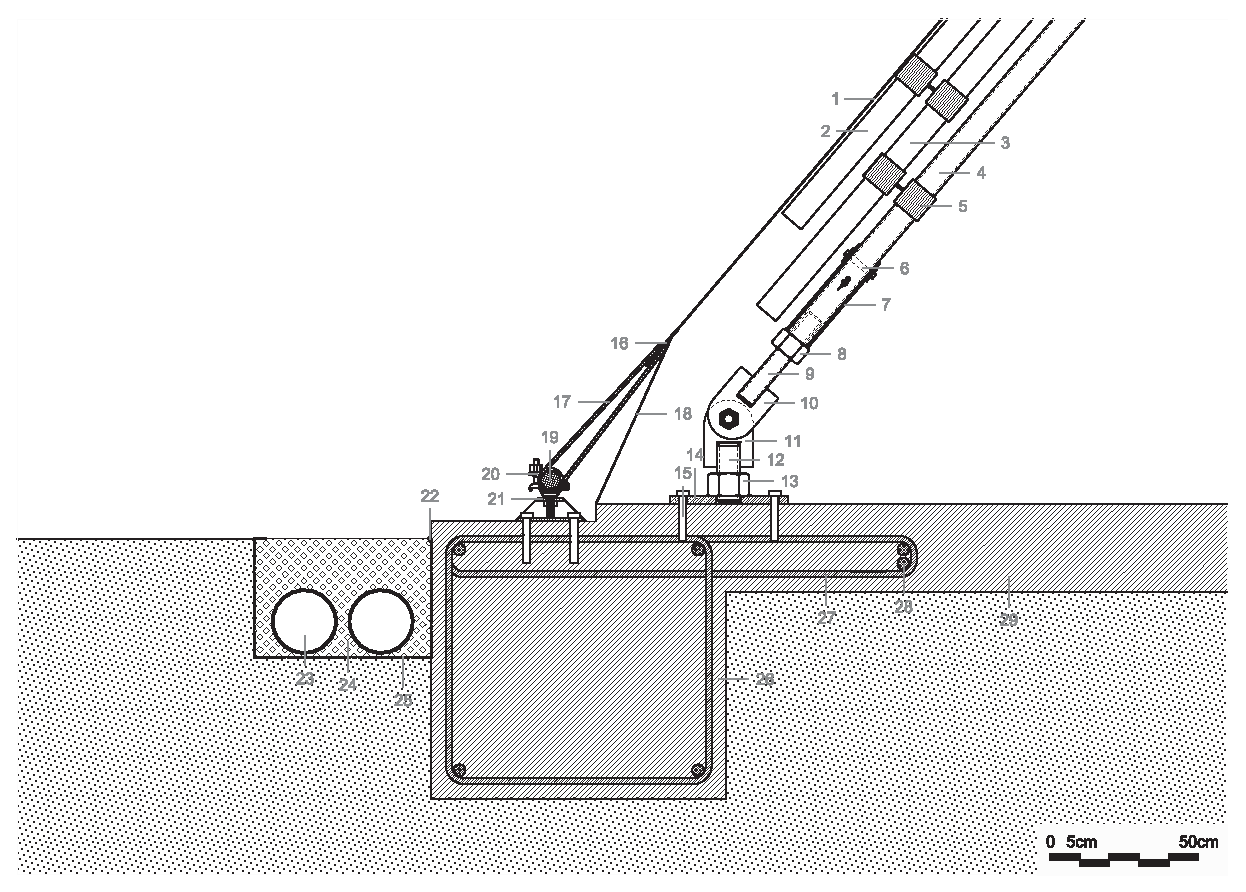
\includegraphics[width=\textwidth]{image13}
	\caption{Section on the footer}
	\label{fig:9}
\end{figure}

\subsection{Flexural strength of the tubes}
%------------------------------------------
The characteristic flexural strength ($\sigma_{k,flex}$) of the GFRP tube has a critical impact on the structure’s reliability because in this particular application stresses in the tubes are mainly due to bending. Thus, it was important to confirm the manufacturer’s value by assays. 
Three-point flexural tests were led with and without connexions (tightening torque set to 20Nm) to determine the characteristic strength according to the protocol of the Eurocode (Annex D) :
\begin{equation}
\sigma_{k,flex}=\overline{\sigma}(1-k_n\sigma_x)
\end{equation}

For five tests, the factor $k_{n,5\%}$ is 1.80 , assuming a normal distribution. One can note that the connections scatter the results more (Table 1). Finally, the manufacturer value of \SI{400}{\mega\pascal} (ASTM D790) was confirmed and retained for further calculations.
\begin{table}[h]
\centering
	\ra{1.1}
 	\begin{tabular}{@{}l r r r r r r @{}}
	\toprule
	Connection & $\sigma_1$ & $\sigma_2$ & $\sigma_3$ & $\sigma_4$ & $\sigma_5$ & $\sigma_{k}$ \\
	\midrule
	Without & 456 & 441 & 445 & 460 & 477 & 430 \\
	With (20\,Nm) & 444 & 478 & 434 & 479 & 427 & 408 \\
	\bottomrule
	\end{tabular}\label{tab:sigma}
	\caption{Three-point flexural resistance of the GFRP tubes (\SI{}{\mega\pascal}).}
\end{table}

\subsection{Partial safety factors}
%------------------------------------------
The partial coefficients of material resistance used in the project are calculated according to the Eurocomp (Table 2). The short-term coefficient proposed in the Eurocomp ($\gamma_{st} = 1.3$) was raised to consider the critical stage of erection, where the deformations are not controlled accurately. 

\begin{table}[h]
\label{tab:2}
\centering
	\ra{1.1}
 	\begin{tabular}{@{}l r r @{}}
	\toprule
	Time scale 	& $\gamma$		& $\sigma_{d}$\\
	\midrule
	Short-term 	& $ 2.0$ 			& 200 \\
	Long-term 	& $ 3.0$ 			& 133 \\
	\bottomrule
	\end{tabular}\label{tab:gamma}
	\caption{Short-term and long-term values for material resistance. $\gamma$ is the partial coefficient for safety factor. $\sigma_{d}$ is the flexural design strength.}
\end{table}

Note that designers should take care about long-term effects in permanently loaded pultruded composite materials subjected to creeping and relaxation \citep{Kotelnikova-Weiler2012}. Here, it is reflected in a high partial coefficient for long-term effects.


%\newpage \phantom{abc}
\clearpage

\section{Cost analysis}
%------------------------------------------
\subsection{Overall cost for the client}
The overall cost of the project -- that is the amount of money paid by the client -- was estimated to 324\,000~€ excluding taxes (see \cref{fig:budget}). This price includes all the possible costs related to the construction of the project~: the cost of the main building (masonry, doors, gridshell, envelop, fittings, heating, electricity, lightning, drainage, sewage, etc.), the cost of the service building, the cost of pedestrian pathways, the cost of the design studies, etc.

However, this cost does not take into account all the (free) man-hours spent by the volunteers to prefabricate, assemble, erect and brace the gridshell. The real cost of the gridshell system, when a cost is put on this labor, is estimated in \cref{sec:gs_cost}.

Moreover, this project required a lot of design studies and tests to verify the material properties and to validate the strength of key elements such as the swivel coupler with its EPDM layer, the sleeve system and the ground anchorage. The real cost of the studies was by far higher than what was really charged to the client and the difference must be regarded as an investment from the company T/E/S/S. In the same manner, people from the laboratory gave a consistent support during the construction stage as they were the only available experienced workers familiar with the construction of elastic gridshells in composite material \cite{Douthe2010,Baverel2012} and this labor was not charged back to the client.

The project was favorably accepted by the client based on the estimation that the cost of the gridshell would not be more expensive by 30\% than renting a simple tent. The rental of a 400~m\textsuperscript{2} tent with its floor was evaluated to 110\,000~€ for a period of time of 18 months. Retrospectively this target was met, especially as the cathedral was finally used for almost two years and a half, far more than the 18 months expected initially, and with no additional cost because the diocese owned the building

\begin{figure}[h]
\begin{fullpage}
\centering
	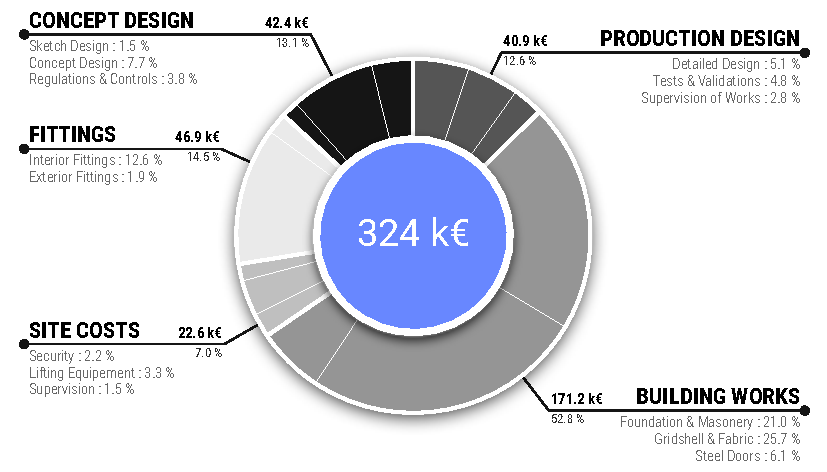
\includegraphics[]{budget}\vspace{10pt}
	\caption{Cost allocation for the whole project. This is the estimated overall final cost charged to the client. Prices are given excluding taxes (V.A.T).}
	\label{fig:budget}
	%
	\vspace{2cm}
	%
	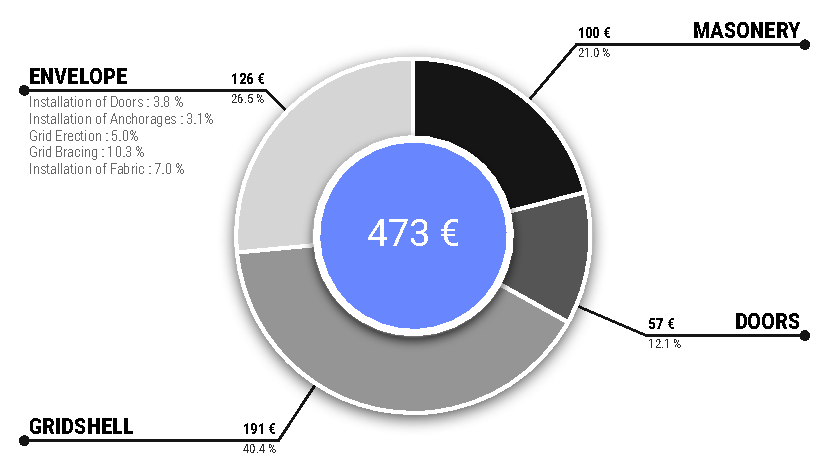
\includegraphics[]{building}\vspace{10pt}
	\caption{Cost allocation per square meter of covered area. The cost of design is not included as it would not be representative. Prices are given excluding taxes (V.A.T).}
	\label{fig:building}
	\end{fullpage}
\end{figure}

\subsection{Cost details for the building}\label{sec:gs_cost}
Here we present the cost details for the main building, that is the cathedral itself. We try to understand what is the true cost of the gridshell system in this particular project and we thus eliminate side costs (for instance the cost of fittings, the cost of the pedestrian pathways, the cost of the service building, etc.). The cost allocation is presented per square meter of covered area in \cref{fig:building}. The total price for the building, excluding studies, is 473~€/m\textsuperscript{2}. It is composed of :
\begin{itemize}
\item  100~€/m\textsuperscript{2}~: the cost of masonry works (levelling, footings, slab, drainage) detailed in \cref{tab:masonry}. This construction works were made by a professional contractor named BATEM.
\item  248~€/m\textsuperscript{2}~: the cost of the superstructure (anchorages, gridshell, membrane covering and doors) detailed in \cref{tab:superstructure}. This price includes the labor of the volunteers (35~€/hour) and all the costs associated to construction of the structure, including the renting of all the necessary equipments (cranes, arial buckets, etc.).
\item  126~€/m\textsuperscript{2}~: the cost of the envelope (lacing rod, fabric, installation) detailed in \cref{tab:superstructure}. This construction works were made by a professional contractor named ESMERY CARON.
\end{itemize}

Here, the global amount of studies was charged around 83\,300~€, that is 248~€/m\textsuperscript{2} (see \cref{fig:budget}). This heavy cost was compensated by the fact that volunteers provided a lot of free labor (see \cref{fig:manhours}). In a more standard commercial context, the design process would be optimized too and the price of studies would go down to 15\% to 20\% of the price of the building, that is 70 to 95~€/m\textsuperscript{2}. This would bring the final price of the building to 550~€/m\textsuperscript{2}. This price is clearly high if only its sheltering capability is required regarding other technologies.. However, if more than sheltering is mandatory, the quality and singularity of the space created here is probably worth the price ; then this technology becomes a lot more affordable than existing traditional systems that can materialized free-forms.

\subsection{Strengths and weaknesses}
In this project the prefabrication process represents almost half of the cost in man-hours (see \cref{fig:manhours}). The manufacturing of the grid (cutting pipes, marking nodes, preassembling swivel couplers, sleeves and anchorages, etc.) could easily be automated. Composite materials such as GFRP are easy to cut, mill and drill. Small robot arms can do the job quickly with a better accuracy. This idea has been tested in a workshop at the Ecole des Ponts ParisTech in septembre 2016.\footnote{See the video of the construction of a 50~m\textsuperscript{2} wooden gridshell in the workshop \textquote{Building Free Froms}~: \url{http://thinkshell.fr/freeform-wooden-gridshell-2016/}.} More over, a numerical production process would allow to answer quickly to a variety of forms with the same equipment and industrial process.

Lots of man-hours are spent in the installation of the sleeve system (88~h). That represents 35~\% of the man-hours spent in the grid prefabrication. This part should be reimplemented to allow a simpler and faster installation. Similarly, the connection should be redesigned to avoid the application of the EPDM protection layer and to allow a faster positioning and fastening as it represents 23~\% of the man-hours spent in the prefabrication of the grid. This would also be a preponderant factor of improvement in the bracing stage although this cost is not detailed in \cref{tab:manhours}.

At first sight it seems that the time spending assembling the grid on the construction site -- which represents 22~\% of the man-hours, see \cref{fig:manhours} -- can not easily be reduced. However, the grid system could be divided into transportable modules. These modules would be preassembled in the factory to increase the speed and quality of the production and to minimize on-site works. Thanks to the intrinsic grid kinematic, modules can be folded for transportation. Once on site, modules are unfolded and connected to each other to form the primary flat grid. This idea was tested successfully in two wooden gridshell projects of 50~m\textsuperscript{2} each, with students of the Ecole National d'Architecture de Toulouse and Ecole National d'Architecture de Grenoble in June 2016.\footnote{Construction of two wooden gridshell pavilions : \url{http://www.lemoniteur.fr/article/a-toulouse-les-architectes-se-rassemblent-sous-le-meme-pavillon-32398196}.}

Bracing is yet another costly stage as it accounts for almost 30~\% of the man-hours (see \cref{fig:manhours}). This work is not easily parallelizable as it requires working at height with proper lifting equipments such as cherry pickers. Thus almost a small and qualified team can do the job. For instance, on the gridshell of Créteil, the team was composed of 6 workers using two aerial lifts. This team spent three full days to complete this task, that is the same amount of days required to assemble the grid and lift it up. Several attempt have been made during this thesis to answer this problematic. The first attempt was to use a bidirectional cable network to brace the grid. The network is installed at the ground level before the grid is deformed. Thus, work at height is reduced to a minimum. The second attempt is a larger thought on the envelope of such structures and tries to tackle two issues with a thin fibre-reinforced concrete skin~: the fact that bracing with a third direction of tubes is time consuming ; and the fact that membrane covering is not adapted for permanent buildings.

\clearpage

\begin{figure}[h]
\centering
\begin{leftfullpage}
	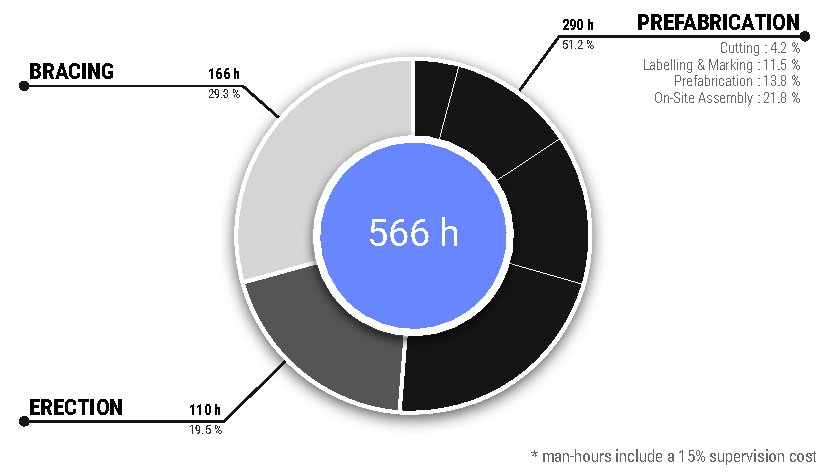
\includegraphics[]{manhours}\vspace{10pt}
	\caption{Allocation of the man-hours spent by the volunteers on the fabrication of the gridshell. A 15\% increase is considered to take into account coordination and supervision of the individual tasks. See \cref{tab:manhours} for detailed data.}
	\label{fig:manhours}
\end{leftfullpage}
\end{figure}
\begin{table}[h]
\centering
\ra{1.1}
\begin{fullpage}
 	\begin{tabularx}{\textwidth}{@{}Xrrrr@{}}
	\toprule
											& \multicolumn{2}{c}{Unit Task} 		& \multicolumn{2}{c}{Man-Hours}	 	\\
	\cmidrule(l){2-3} \cmidrule(l){4-5}
 	Item 										& Worker 		& Duration		& Quantity 		& Hours			\\ 
	\midrule
	%
	\addlinespace[10pt]
	\textbf{Workstation \textquote{Cutting}}			& \tablebf{4}	& 				&				& \tablebf{20.53}	\\ 
	Pick a raw tube from the stock					& 2 			& 1'\,00''			& 176			& 5.87 			\\ 
	Mark it and cut it at right length					& 2 			& 2'\,00''			& 176			& 11.73			\\ 
	Put it into the labelling stock					& 2  			& 0'\,30''			& 176			& 2.93 			\\ 
	%
	\addlinespace[10pt]
	\textbf{Workstation \textquote{Labelling}}			& \tablebf{5}	&				&				& \tablebf{56.64} 	\\ 
	Pick a tube from the labelling stock				& 2 			& 1'\,00''			& 176			& 5.87 			\\ 
	Label it at start and end						& 2  			& 1'\,00''			& 176			& 5.87 			\\ 
	Mark the position of connection collars			& 1  			& 0'\,30''			& 2260			& 18.83			\\
	Mark the position of sleeves					& 1  			& 0'\,30''			& 250			& 2.08			\\
	Mark the position of anchorages				& 1  			& 0'\,30''			& 127			& 21.06			\\
	Put it into the prefabrication stock					& 2  			& 0'\,30''			& 176			& 2.93 			\\ 
	%
	\addlinespace[10pt]
	\textbf{Workstation \textquote{Prefabrication}}		&  \tablebf{6}   	&				& 				& \tablebf{67.75} 	\\ 
	Pick a tube from the prefabrication stock			& 2 			& 1'\,00''			& 176			& 5.87 			\\ 
	Put the EPDM ribbon						& 1 			& 0'\,30''			& 2260			& 18.83 			\\ 
	Prefix the swivel collar on the tube				& 1 			& 0'\,30''			& 565			& 4.71 			\\ 
	Glue	the sleeves							& 3  			& 2'\,00''			& 250			& 25.00			\\
	Drill pin holes for the sleeves					& 1  			& 1'\,00''			& 250			& 4.16			\\
	Fix sleeve pins 								& 1  			& 1'\,30''			& 250			& 6.25			\\
	Put it into the final stock						& 2  			& 0'\,30''			& 176			& 2.93 			\\ 
	%
	\addlinespace[10pt]
	\textbf{Workstation \textquote{Site Assembly}}		&  \tablebf{12}   &				& 				& \tablebf{107.34} 	\\ 
	Connect the sleeves with steel rods 				& 5 			& 5'\,00''			& 125			& 52.08 			\\ 
	Pick a tube and position it in the grid 				& 2 			& 3'\,00''			& 176			& 17.60 			\\ 
	Install swivel couplers (HV)					& 1 			& 2'\,00''			& 565			& 18.83 			\\
	Controlled tightening of couplers (HV)			& 1 			& 1'\,00''			& 1130			& 18.83 			\\ 
	%
	\addlinespace[10pt]
	{Workstation \textquote{Grid Erection}}			& {12}   		& 8:00'\,00''		& 1				& {96.00} 	\\ 
	{Workstation \textquote{Grid Bracing}}			& {6}   		& 8:00'\,00''		& 3				& {144.00} 	\\ 
	%
	\addlinespace[10pt]
	\midrule
	Grid prefabrication 							& 			& 				&				&{252.00}  		\\
	Grid erection 								& 			& 				&				&{96.00}  			\\
	Grid bracing 								& 			& 				&				&{144.00}  		\\
	Cost of supervision (15\%)					& 			&				&				& {74.00}  			\\
	\textbf{Total} 								& 			& 				&				& \tablebf{566.00}  	\\
	\bottomrule
 	\end{tabularx}
	\vspace{10pt}
	\caption{Man-hours spent by the volunteers on the fabrication of the gridshell. A 15\% increase is considered to take into account coordination and supervision of the individual tasks. See \cref{fig:manhours} for a graphical representation of these data.}
	\label{tab:manhours}
\end{fullpage}
\end{table}

\begin{figure}[h]
\centering
\begin{leftfullpage}
	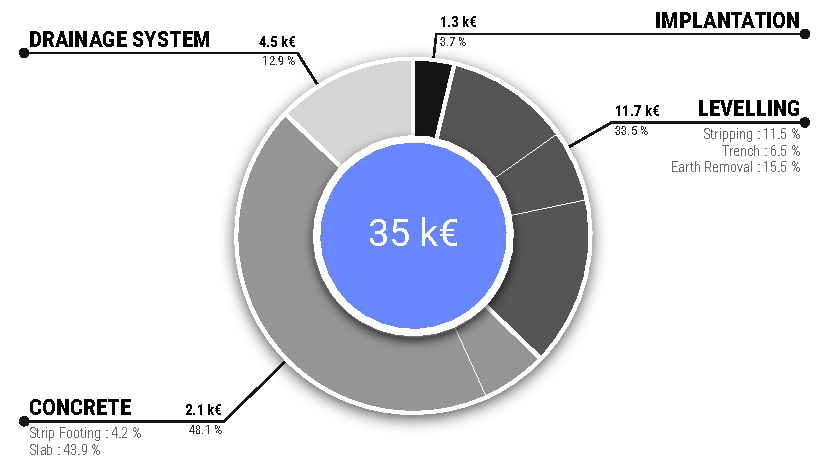
\includegraphics[]{masonry}\vspace{10pt}
	\caption{Cost allocation for masonry works. Prices are given excluding taxes (V.A.T). Only costs associated to the structure are reported here ; for instance the works for the equipment slab and the pathways are omitted. See \cref{tab:masonry} for detailed data.}
	\label{fig:masonry}
\end{leftfullpage}
\end{figure}
\begin{table}[h]
\centering
\ra{1.1}
\begin{fullpage}
 	\begin{tabularx}{\textwidth}{@{}Xlrrr@{}}
	\toprule
 	Item	 							& Unit				& Quantity		& U.P. (€)			& Price (€) 			\\ 
	\midrule
	\addlinespace[10pt]
	Building implantation 				& 					& 1			& 1\,300.00		& 1\,300.00  			\\
	%
	\addlinespace[10pt]
	\textbf{Leveling works } 				& 					& 			& 				& \tablebf{11\,680.00}  			\\
	Top soil stripping  					& m\textsuperscript{2}	& 400		& 10.00			&  4\,000.00  			\\
	Trench for concrete strip footing  		& ml					& 76			& 30.00			&  2\,280.00  			\\
	Earth removal  						& m\textsuperscript{3}	& 180		& 30.00			&  5\,400.00  			\\
	%
	\addlinespace[10pt]
	\textbf{Concrete} 					& 					& 			& 				& \tablebf{17\,400.00}  	\\
	Concrete strip footing (200~kg/m\textsuperscript{3} steel) & ml		& 70			& 30.00			&  2\,100.00  			\\
	Concrete slab (x2 welded wire mesh) 	& m\textsuperscript{2}	& 340		& 45.00			&  15\,300.00  			\\
	%
	\addlinespace[10pt]
	\textbf{Drainage systems} 				& 					& 			& 				& \tablebf{4\,500.00}  	\\
	French drain (x2 \O 100~mm pipes)		& ml					& 70			& 30.00			&  2\,100.00  			\\
	Precast concrete inspection chamber 	& 					& 1			& 400.00			&  400.00  			\\
	Drain line (PVC \O 125~mm pipe)		& ml					& 30			& 30.00			&  900.00  			\\
	Pre-assembled channel drain			& ml					& 10			& 110.00			&  1\,100.00  			\\
	%
	\addlinespace[10pt]
	\midrule
	\textbf{Masonry works} 				& €/m\textsuperscript{2}	& 350 		& \tablebf{100}		& \tablebf{34\,880.00}  	\\
	\bottomrule
 	\end{tabularx}
	\vspace{10pt}
	\caption{Cost details for masonry works. Prices are given excluding taxes (V.A.T). Only costs associated to the structure are reported here ; for instance the works for the equipment slab and the pathways are omitted. See \cref{fig:masonry} for a graphical representation of these data.}
	\label{tab:masonry}
\end{fullpage}
\end{table}


\begin{figure}[h]
\centering
\begin{leftfullpage}
	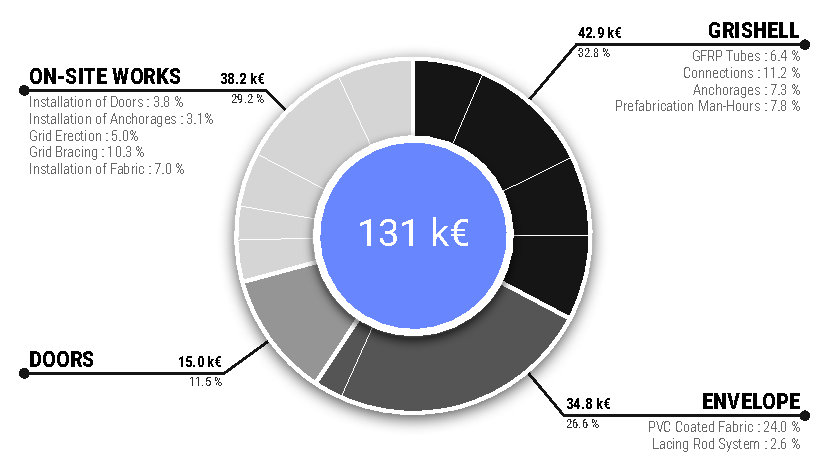
\includegraphics[]{superstructure}\vspace{10pt}
	\caption{Cost allocation for the superstructure. On-site works are isolated to identify pure manufacturing costs of the gridshell, the envelope and the doors. To this end, the cost of the man-hours provided by the volunteers to prefabricate the grid has been assessed and allocated. See \cref{tab:superstructure} for detailed data.}
	\label{fig:superstructure}
\end{leftfullpage}
\end{figure}
\begin{table}[h]
\centering
\ra{1.1}
\begin{fullpage}
 	\begin{tabularx}{\textwidth}{@{}Xlrrr@{}}
	\toprule
 	Item	 							& Unit				& Quantity		& U.P. (€)		& Price (€) 			\\ 
	\midrule
	\addlinespace[10pt]
	\textbf{Manufacturing of the gridshell} 	& 					& 			& 				& \tablebf{42\,853}  	\\
	GRFP tube (\O 42~mm)				& ml					& 2304		& 3.66			&  8\,433  			\\
	Swivel connector (42x42~mm)			& 					& 1295		& 3.95			&  5\,115  			\\
	Swivel connector (42x49~mm)			& 					& 135		& 4.18			&  564  			\\
	EPDM layer (1302x40x1.5~mm ribbon)	& 					& 2775		& 0.36			&  1131  			\\
	Welded steel sleeve system			& 					& 150		& 50.00			&  7\,500  			\\
	ARALDIT 2047 glue (480~ml cartridge)	& 					& 8			& 45.00			&  360 			\\
	Ground anchorage (welded steel)		& 					& 120		& 80.00			&  9\,600  			\\
	Man-hours (prefabrication)			& h 					& 290		& 35.00			& 10\,150			\\
	%
	\addlinespace[10pt]
	\textbf{Manufacturing of the envelope}	& 					& 			& 				& \tablebf{34\,769}  	\\
	GFRP lacing rod (\O 32~mm) 			& ml 					& 96			& 14.00			&  1\,134  			\\
	Steel clip for the rod					&  					& 125		& 15.00			&  1\,875  			\\
	Swivel collar (\O 34~mm)				& 					& 120		& 3.50			&  420  			\\
	PVC coated fabric					& m\textsuperscript{2}	& 550		& 50.00			&  27\,500  		\\
	Option for transparent inclusion			& 					& 12			& 320.00			&  3\,840  			\\
	%
	\addlinespace[10pt]
	\textbf{Manufacturing of the steel doors} 					& 					& 			& 				& \tablebf{15\,000}  	\\
	Main door 						& 					& 1			& 10\,000.00		&  10\,000  		\\
	Small door  						&					& 1			& 5\,000.00		&  5\,000 			\\
	%
	\addlinespace[10pt]
	\textbf{On-site works of installation} 		& 					& 			& 				& \tablebf{33\,365}  	\\
	Installation of the doors				& 					& 1			& 5\,000.00		&  5\,000  			\\
	Installation of the anchorages and clips	& h					& 90			& 45.00			&  4\,050  			\\
	Grid erection 						& h					& 110		& 35.00			&  3\,850  			\\
	\quad {cranes (x2 35T)}				& h					& 24			& 110.00			&  2\,640  			\\
	Grid bracing 						& h					& 167		& 45.00			&  7\,515  			\\
	\quad {aerial bucket (x2)}				& 					& 1			& 6\,000.00		&  6\,000  			\\
	Installation of fabric 					& 					& 1			& 9\,165.00		&  9\,165  			\\
	%
	\addlinespace[10pt]
	\midrule
	\textbf{Total} 						& €/m\textsuperscript{2}	& 374		&  \tablebf{363}		& \tablebf{130\,842}  	\\	
	Cost of structure					&  					& 			& 265			& {92\,622}  		\\
	Cost of installation					& 					& 			& 109			& {38\,220}  		\\
	\bottomrule
 	\end{tabularx}
	\vspace{10pt}
	\caption{Cost details for the superstructure. On-site works are isolated to identify pure manufacturing costs of the gridshell, the envelope and the doors. To this end, the cost of the man-hours provided by the volunteers to prefabricate the grid has been assessed and allocated. Prices are given excluding transport costs and excluding taxes (V.A.T ). Spare quantities are included. See \cref{fig:superstructure} for a graphical representation of these data.}
	\label{tab:superstructure}
\end{fullpage}
\end{table}

\clearpage

\section{Conclusions}
% ------------------------------------------
This paper has presented the different steps for the design of a gridshell in composite material : a Temporary Cathedral at Créteil, in Paris suburb, in 2013. The first step was the optimization of the shape in order to avoid local concentrations of curvature. The second step showed a tool to automatically mesh a surface using the compass method. With this tool, the orientation of the mesh is studied according to structural and architectural criterions. The last steps showed the structural analysis of the gridshell and how to get the as-built geometry from the analysis model.
Architecturally, the structure offers a very interesting space where the textual richness of the tubes against the membrane accentuates the reading of the complex curved surfaces.

This project demonstrates that gridshells in composite material are suitable for constructing freeform buildings. However, the long-term behavior of these materials needs to be better characterized to extend their lifespan.

At the moment, further developments are conducted by the laboratory to take account for torsional effects and non axisymmetric sections in such structures, as it is studied in \citep{Barnes2013}.

\subsection{Acknowledgements}
% ------------------------------------------
The authors would like to thank the Catholic Church of Créteil for their trust and their courage, which permitted to get into this ambitious and successful project. They also want to greet the engineers from T/E/S/S, which have developed this challenging project during 18th months. They also thank the firm Viry for the supervision of construction works, including the delicate erection stage.

\clearpage
\bibliographystyle{alpha}
\bibliography{../library}
